% !TeX program = lualatex
% !BIB program = biber
\documentclass[12pt,letterpaper]{article}

\usepackage[margin=2.54cm,headheight=15pt,headsep=12pt]{geometry}
\usepackage{fontspec}
\setmainfont{Times New Roman}
\setmonofont{Consolas}[Scale=MatchLowercase]

\usepackage{caption}
\usepackage[spanish,es-tabla]{babel}
\AtBeginDocument{\spanishplainpercent}
\usepackage{csquotes}
\usepackage{microtype}
\usepackage{setspace}
\usepackage{ragged2e}
\usepackage{fancyhdr}
\usepackage{titlesec}
\usepackage{amsmath,amssymb}
\usepackage{booktabs}
\usepackage{longtable}
\usepackage{array}
\usepackage{tabularx}
\usepackage{threeparttable}
\usepackage{pdflscape}
\usepackage{graphicx}
\usepackage{xcolor}
\usepackage{tikz}
\usetikzlibrary{arrows.meta,positioning,shapes.geometric,fit,backgrounds}
\usepackage{enumitem}
\usepackage{siunitx}
\usepackage[hidelinks,breaklinks=true]{hyperref}

\sisetup{
  output-decimal-marker = {,},
  group-separator = {.},
  group-digits = integer,
  group-minimum-digits = 4,
  detect-all
}

\usepackage[
  backend=biber,
  style=apa,
  sortcites=true
]{biblatex}
\DeclareLanguageMapping{spanish}{spanish-apa}
\addbibresource{referencias.bib}
\setlength{\bibhang}{1.27cm}
\renewcommand*{\bibfont}{\normalfont\normalsize\RaggedRight}
\appto\bibsetup{\RaggedRight}
\def\UrlBreaks{\do\/\do\_\do\.\do\-}
\AtBeginDocument{\Urlmuskip=0mu\relax}
\hyphenation{FastAPI LightGBM MediFlow PostgreSQL Vite}

% Formato APA 7: numeración de páginas superior derecha desde la página 1, sin encabezado abreviado.
\pagestyle{fancy}
\fancyhf{}
\fancyhead[R]{\thepage}
\renewcommand{\headrulewidth}{0pt}
\fancypagestyle{plain}{
  \fancyhf{}
  \fancyhead[R]{\thepage}
  \renewcommand{\headrulewidth}{0pt}
}

% Encabezados APA 7 sin numeración automática.
\setcounter{secnumdepth}{0}
\titleformat{\section}{\normalfont\normalsize\bfseries\centering}{}{0pt}{}
\titlespacing*{\section}{0pt}{14pt}{6pt}
\titleformat{\subsection}{\normalfont\normalsize\bfseries\raggedright}{}{0pt}{}
\titlespacing*{\subsection}{0pt}{12pt}{4pt}
\titleformat{\subsubsection}{\normalfont\normalsize\bfseries\itshape\raggedright}{}{0pt}{}
\titlespacing*{\subsubsection}{0pt}{10pt}{2pt}
\titleformat{\paragraph}[runin]{\normalfont\normalsize\bfseries}{}{0pt}{}[.]
\titlespacing*{\paragraph}{1.27cm}{6pt}{0.5em}
\titleformat{\subparagraph}[runin]{\normalfont\normalsize\bfseries\itshape}{}{0pt}{}[.]
\titlespacing*{\subparagraph}{1.27cm}{6pt}{0.5em}

% Título de Referencias según nivel 1 APA 7 (centrado y en negrita, en página nueva).
\defbibheading{bibliography}[\refname]{%
  \clearpage
  \section*{#1}%
}

% Tablas y figuras en formato APA 7: etiqueta en negrita arriba y título en cursiva debajo.
\captionsetup{
  justification=raggedright,
  singlelinecheck=false,
  labelsep=newline,
  labelfont=bf,
  textfont=it,
  skip=6pt
}

% Alineación izquierda y sangría de primera línea de 1,27 cm (0,5 pulgadas).
\RaggedRight
\setlength{\parindent}{1.27cm}
\setlength{\parskip}{0pt}
\doublespacing
\setlength{\emergencystretch}{3em}
\setlength{\tabcolsep}{3.5pt}

% Utilidades editoriales para notas APA y bloques de código en interlineado sencillo.
\newcommand{\apanota}[1]{%
  \par\vspace{4pt}%
  {\singlespacing\footnotesize\RaggedRight\noindent\textit{Nota.} #1\par}%
}
\newcolumntype{L}[1]{>{\RaggedRight\arraybackslash}p{#1}}
\newcolumntype{R}[1]{>{\RaggedLeft\arraybackslash}p{#1}}
\newcolumntype{C}[1]{>{\Centering\arraybackslash}p{#1}}
\newcolumntype{Y}{>{\RaggedRight\arraybackslash}X}

\graphicspath{{figuras/}}

\hypersetup{
  pdftitle={MediFlow},
  pdfauthor={Juan David Campo Mercado; Daniel Alejandro Rincón Navarro; Carlos David del Castillo Mercado},
  pdfsubject={Data Challenge HUN 2026 -- Informe técnico APA 7}
}

\begin{document}

% Portada adaptada APA 7 y Resumen (páginas 1 y 2)
% evidencia:E03,E08,E13,E18

\thispagestyle{fancy}
\begingroup
\centering
\vspace*{2.5\baselineskip}

{\bfseries MediFlow}\par
\vspace{1.5\baselineskip}

Juan David Campo Mercado\par
Daniel Alejandro Rincón Navarro\par
Carlos David del Castillo Mercado\par
\vspace{0.5\baselineskip}
Universidad del Norte\par
19 de noviembre de 2026\par
\endgroup

\vfill
\begin{flushleft}
{\singlespacing\footnotesize\RaggedRight
\textit{Nota documental.} El título exacto, el orden de autoría y la omisión de campos de asignatura, docente y tutor corresponden a decisión editorial expresa para este informe, adaptando la portada estudiantil de la séptima edición de las normas APA. La fecha indicada es documental y no constituye una fecha oficial de entrega del certamen. Base técnica verificada en el repositorio: commit \nolinkurl{803c1a1f866a978cce8b4622269ccfb4749ba59e}, artefacto web empaquetado \texttt{v2.0} (corte exclusivo \texttt{2026-07-17}, huella SHA-256 \nolinkurl{be8252b056377f8820808a518095235c1215b6ad5c3466a781bad6a0f0ad1e28}).\par}
\end{flushleft}
\clearpage

% evidencia:E08,E13,E18
\section{Resumen}

\noindent MediFlow es una herramienta analítica de apoyo a la planificación operacional del Hospital Universidad del Norte (HUN) construida sobre agregados compatibles con el modelo OMOP CDM v5.4 bajo tres ejes: comprender el flujo asistencial, predecir la demanda diaria y explorar escenarios paramétricos de decisión. Sobre \num{1706001} registros históricos de visitas entre el 1 de enero de 2023 y el último día completo de demanda (\texttt{2026-07-16}; corte exclusivo \texttt{2026-07-17}), la deduplicación SQL consolida \num{1477742} llegadas únicas, el censo por etapas de \texttt{visit\_detail} aplica recorte estadístico $p_{99{,}9}$ y la auditoría de calendario verifica desfase temporal cero. Se documentan por separado dos familias predictivas a 1--7 días evaluadas en 26 pliegues \textit{walk-forward}: el experimento puntual LightGBM Poisson con nivel local y factores externos aceptados (\texttt{lgbm\_final}) reduce el error WAPE diario global de 18,0\,\% en la línea base a 15,6\,\% en regresión de Poisson estratificada y a 10,5\,\% final (mejora relativa archivada de 41,6\,\%; 8,4\,\% en Urgencias y 11,0\,\% en Rehabilitación frente a 43,5\,\% en Tratamiento Urgencias), mientras que el artefacto cuantílico servido en la aplicación web (\texttt{v2.0}, $p_{10}/p_{50}/p_{90}$) registra sobre 182 días un WAPE archivado de 8,91\,\% en Urgencias (cobertura 78,57\,\%), 11,08\,\% en Rehabilitación (64,29\,\%) y 42,18\,\% en Tratamiento Urgencias (73,08\,\%). A 120 días se distinguen los resultados archivados del 3 de noviembre de 2026 (WAPE 15,7\,\%, cobertura 86,5\,\%) de la corrida empaquetada en el artefacto servido. La capa operacional integra dimensionamiento Erlang~C bajo tasas y duraciones supuestas (15 frente a 12 equipos equivalentes en Urgencias 06--12\,h en demanda $p_{90}$; 70 frente a 42 en Rehabilitación), contraste de Ley de Little (\num{277,52} pacientes en población alineada frente a \num{277,47} de media horaria y \num{284,01} en la referencia híbrida del bundle) y simulación horaria de altas tempranas (35\,\% adelantadas reducen las horas rojas de 9,32\,\% a 6,26\,\% manteniendo el pico en 359). Los resultados justifican validación operativa supervisada, pero no demuestran beneficio clínico ni sustituyen la verificación presencial de dotación y camas habilitadas.

\indent\textit{Palabras clave:} flujo hospitalario, OMOP CDM, pronóstico de demanda, validación temporal, Erlang~C, Ley de Little, planificación operacional.

\clearpage

% Sección 1: Introducción y objetivos (en APA 7 el título repetido actúa como encabezado de nivel 1)
% evidencia:E01,E02,E03

\section{MediFlow}

La gestión operativa de un hospital de alta complejidad exige articular la anticipación de llegadas diarias con el comportamiento de la permanencia intrahospitalaria y la distribución horaria de los recursos de atención. En el Hospital Universidad del Norte (HUN), la disponibilidad de un repositorio clínico estructurado bajo el estándar Observational Medical Outcomes Partnership Common Data Model (OMOP CDM) versión 5.4 \parencite{ohdsi54} abre la posibilidad de analizar trayectorias agregadas sin exponer registros individuales de pacientes; sin embargo, dicha representación administrativa carece de tablas de capacidad física instalada, camas censales habilitadas y dotación contractual de personal por turno \parencite{mediflow2026informe}. Ante esa restricción estructural, MediFlow se concibe como una herramienta de apoyo a la planificación que sigue el hilo conductor de \textbf{comprender, predecir y decidir}: reconstruye el flujo histórico por etapas, evalúa la incertidumbre de la demanda con validación temporal estricta y traduce pronósticos y reglas de permanencia en escenarios paramétricos interpretables con supuestos explícitos.

El aporte defendible del proyecto reside en la integración trazable de cuatro capas técnicas que permanecen desacopladas de los datos individuales en el despliegue: extracción SQL agregada de solo lectura en origen, modelado predictivo con evaluación temporal de origen móvil y explicabilidad aditiva, análisis operacional basado en teoría de colas y balance de flujo, e interfaces interactivas (aplicación web FastAPI/React y tablero histórico en Power BI). En coherencia con la evidencia disponible, el sistema no afirma haber demostrado una reducción clínica observada en los tiempos de espera ni una asignación óptima sobre recursos reales del hospital; todo escenario cuantificado se presenta como hipótesis operacional sujeta a contraste con la capacidad y las marcas temporales del sistema de información hospitalario (HIS).

\subsection{Objetivos y alcance editorial}

Como síntesis editorial del trabajo desarrollado por el equipo para el Data Challenge HUN 2026, el objetivo general consiste en analizar el flujo de pacientes y apoyar la planificación operacional del HUN mediante pronósticos de demanda con intervalos de incertidumbre y simulaciones interpretables bajo supuestos explícitos. De este propósito se desprenden cinco objetivos específicos: (a) reconstruir la demanda por servicio, las etapas de atención, las transiciones entre áreas y el censo horario a partir de agregados OMOP; (b) auditar la calidad, la completitud, la consistencia temporal y el aporte empírico de factores externos mediante protocolos anti-fuga; (c) contrastar modelos predictivos de corto y largo horizonte con métricas libres de explosión por ceros y evaluación temporal estricta; (d) cuantificar escenarios paramétricos de dotación equivalente, permanencia promedio y redistribución intradía de egresos; y (e) comunicar las capacidades implementadas, las diferencias entre versiones experimentales y los límites que condicionan una eventual validación clínica. Esta formulación ordena la exposición técnica del informe sin introducir requisitos ajenos a las bases oficiales del certamen.

\subsection{Correspondencia con los requisitos oficiales del certamen}

Las exigencias normativas del proyecto provienen exclusivamente de los términos y condiciones de participación y del enunciado técnico oficial del Data Challenge HUN 2026 \parencite{hun2026terminos,hun2026reto}. Los documentos oficiales establecen como entregables la documentación técnica que consolide metodología, análisis, resultados, conclusiones y recomendaciones; un repositorio en GitHub con el código y recursos autorizados; un enlace interactivo en Power BI; y la sustentación oral cuando corresponda. El enunciado permite abordar uno o varios componentes del flujo hospitalario y no exige emplear todas las tablas clínicas como variables predictoras ni desplegar un piloto asistencial previo en producción.

\begin{table}[htbp]
\caption{Criterios oficiales de evaluación y desempates del Data Challenge HUN 2026}
\label{tab:criterios_oficiales}
{\singlespacing\small
\begin{tabularx}{\textwidth}{@{}L{0.46\textwidth} r Y@{}}
\toprule
Criterio oficial de evaluación & Peso & Bloque principal del informe \\
\midrule
Comprensión del problema y análisis del flujo hospitalario & 15\,\% & Introducción; Datos y reconstrucción del flujo \\
Calidad, preparación e integración de los datos & 15\,\% & Datos y flujo; Calidad, preparación y externos \\
Modelo analítico y/o predictivo y rigor metodológico & 20\,\% & Método analítico y validación; Resultados predictivos \\
Optimización y propuestas de mejora operacional & 20\,\% & Optimización operacional y simulaciones paramétricas \\
Integración de la solución, visualización y dashboard & 15\,\% & Integración, aplicación web y visualización \\
Ingeniería de software, reproducibilidad y documentación & 5\,\% & Ingeniería de software, reproducibilidad y privacidad \\
Presentación, interpretación y recomendaciones accionables & 10\,\% & Discusión, recomendaciones y conclusiones \\
\midrule
Total de la rúbrica oficial & 100\,\% & Cobertura transversal y anexos de trazabilidad \\
\bottomrule
\end{tabularx}}
\apanota{Elaboración basada en \textcite{hun2026terminos}, página~4, secciones 13 y 14, y \textcite{hun2026reto}, página~3. Según la sección~16 de los términos y condiciones (p.~5), los empates se resuelven sucesivamente por optimización y mejora operacional, modelo analítico y rigor metodológico, comprensión del flujo hospitalario y, en último término, valoración conjunta de utilidad, factibilidad y carácter accionable. La redacción en LaTeX, el uso de las normas APA de séptima edición y la extensión del documento obedecen a decisiones editoriales de los autores y no a una imposición de los documentos oficiales del certamen.}
\end{table}

La Tabla~\ref{tab:criterios_oficiales} resume la distribución porcentual de la rúbrica oficial y su correspondencia estructural con los capítulos de este informe. Por rigor normativo, la correspondencia tiene carácter exclusivamente orientador y no introduce subpesos internos ni duplica el peso de un criterio por aparecer tratado de forma transversal entre capítulos. Asimismo, toda distinción entre corridas experimentales archivadas, metadatos inspeccionados del artefacto empaquetado para la web y pruebas locales se mantiene explícita desde la presentación inicial para evitar mezclar evidencia de distinta naturaleza.

% Sección 2: Datos hospitalarios y reconstrucción del flujo asistencial
% evidencia:E03,E06,E07,E19

\section{Datos hospitalarios y reconstrucción del flujo asistencial}

El análisis parte del repositorio PostgreSQL de solo lectura alojado en el esquema institucional compatible con OMOP CDM v5.4 \parencite{ohdsi54,mediflow2026inventario}. En concordancia con el principio de privacidad del certamen y con las decisiones iniciales del equipo, ninguna etapa del flujo analítico descarga filas individuales de pacientes ni identificadores clínicos: todas las extracciones se ejecutan en origen mediante 24 consultas SQL agregadas que exportan únicamente conteos por hora, día, mes o concepto hacia almacenamiento local protegido fuera del control de versiones \parencite{mediflow2026informe,mediflow2026auditoria}.

\subsection{Esquema OMOP disponible frente a uso efectivo y cortes temporales}

Una distinción metodológica indispensable separa las tablas visibles en el catálogo OMOP del subconjunto efectivamente incorporado en los modelos predictivos y simulaciones. Aunque la base hospitalaria expone siete tablas principales de gran volumen ---entre ellas diagnósticos, procedimientos y mediciones de laboratorio---, la presencia de una tabla en el esquema no implica su inclusión automática como predictor. La Tabla~\ref{tab:omop_uso} contrasta la volumetría estimada en el inventario inicial con el uso efectivo dentro del sistema.

\begin{table}[htbp]
\caption{Tablas OMOP inventariadas frente a uso efectivo, granularidad y corte temporal}
\label{tab:omop_uso}
{\singlespacing\small
\begin{tabularx}{\textwidth}{@{}L{0.24\textwidth} r r Y@{}}
\toprule
Tabla OMOP & Filas est. & Tamaño & Uso efectivo y restricciones observadas \\
\midrule
\texttt{procedure\_occurrence} & 47,0\,M & 3,86\,GB & Solo catálogo agregado de frecuencias ($\ge 10$ registros); sin hora de procedimiento; no entra como predictor del modelo \\
\texttt{condition\_occurrence} & 38,6\,M & 3,79\,GB & Solo frecuencias agregadas de conceptos ($\ge 10$ registros); no entra en la matriz de variables del modelo de demanda \\
\texttt{measurement} & 16,6\,M & 15,0\,GB & Solo frecuencias agregadas; faltan \texttt{unit\_concept\_id} y tipo; no se integra como predictor \\
\texttt{concept} & 10,0\,M & 1,07\,GB & Diccionario de traducción de identificadores de concepto a etiquetas legibles \\
\texttt{visit\_detail} & 3,28\,M & 318\,MB & Base efectiva para etapas, duración, transiciones y censo horario; carece de \texttt{person\_id} directo (enlace vía \texttt{visit\_occurrence}) \\
\texttt{visit\_occurrence} & 1,71\,M & 153\,MB & Fuente única para llegadas diarias/horarias; inicio igual a fin en el extracto, inútil para medir estancias \\
\texttt{person} & 912\,k & 92\,MB & Solo cruce SQL para sexo y grupo etario por año de nacimiento (\texttt{13\_llegadas\_diarias\_perfil.sql}) \\
\bottomrule
\end{tabularx}}
\apanota{Volumetría archivada del inventario ejecutado el 15 de octubre de 2026 sobre estimación de catálogo PostgreSQL \parencite{mediflow2026inventario}. La definición de esquema sigue el estándar OMOP CDM v5.4 \parencite{ohdsi54}. En los archivos del repositorio también figuran diferencias respecto de la especificación base: ausencia de \texttt{preceding\_visit\_occurrence\_id}, \texttt{visit\_type\_concept\_id} y \texttt{procedure\_datetime}.}
\end{table}

Asimismo, no existe un único corte temporal universal compartido por todos los productos del proyecto. En las series de demanda extraídas desde \texttt{visit\_occurrence}, el rango cubre desde el 1 de enero de 2023 sin meses vacíos hasta el 16 de julio de 2026 como último día completo, con corte exclusivo automático en \texttt{2026-07-17} implementado en la función \texttt{fecha\_corte} \parencite{mediflow2026inventario,mediflow2026bundle}. Existen registros tardíos sueltos hasta el 13 de agosto de 2026 que se descartan explícitamente para no interpretar un tramo incompleto como semanas de demanda nula. Por su parte, el análisis de balance y censo en Hospitalización extiende la ventana hasta el cierre de las últimas salidas registradas el 18 de julio de 2026 a las 06:00 \parencite{mediflow2026informe}, mientras que el modelo semántico de Power BI opera con parámetro explícito \texttt{FechaCorte = 2026-04-30} \parencite{mediflow2026pbip}. En consecuencia, los resultados de demanda, censo y tablero histórico describen ventanas parcialmente distintas que nunca deben compararse como si compartieran idéntica cohorte.

\subsection{Población de visitas y etapas asistenciales}

Dentro de \texttt{visit\_occurrence}, la unidad de análisis para el pronóstico de demanda corresponde al número de llegadas únicas por \texttt{visit\_concept\_id} y día. La Tabla~\ref{tab:volumen_visitas} detalla la distribución archivada por tipo de visita y la decisión de modelado adoptada. Tres servicios concentran la demanda modelada directamente: Rehabilitación Ambulatoria (código OMOP \texttt{581479}), Urgencias (\texttt{9203}) y Tratamiento Urgencias (\texttt{3045729}). En contraste, Hospitalización (\texttt{9201}) registra apenas 592 visitas principales ($\approx 0{,}5$ por día) en \texttt{visit\_occurrence} y se agrupa junto con 2 registros sin concepto mapeado dentro de la serie residual \texttt{Otros} (código interno \texttt{-1}) para el pronóstico diario, porque evaluar un porcentaje de error relativo cuando la mayoría de los días tiene cero llegadas distorsiona las métricas globales \parencite{mediflow2026inventario}.

\begin{table}[htbp]
\caption{Volumen archivado por tipo de visita principal en \texttt{visit\_occurrence}}
\label{tab:volumen_visitas}
{\singlespacing\small
\begin{tabularx}{\textwidth}{@{}Y r r L{0.24\textwidth}@{}}
\toprule
Tipo de visita (\texttt{visit\_concept\_id}) & Visitas & Prom./día & Decisión analítica \\
\midrule
Ambulatory Rehabilitation Visit (\texttt{581479}) & \num{1089461} & $\approx 827$ & Se modela \\
Emergency Room Visit (\texttt{9203}) & \num{598088} & $\approx 443$ & Se modela \\
Treatment urgency \{Diagnosis\} (\texttt{3045729}) & \num{17858} & $\approx 15$ & Se modela (diario) \\
Inpatient Visit (\texttt{9201}) & \num{592} & $\approx 0{,}5$ & Agrupada en \texttt{Otros} \\
No matching concept (\texttt{0}) & \num{2} & $\approx 0$ & Agrupada en \texttt{Otros} \\
\bottomrule
\end{tabularx}}
\apanota{Cifras archivadas del inventario de la base \parencite{mediflow2026inventario} previas a la agregación temporal estricta por corte; corresponden a registros brutos por concepto en el inventario inicial. El bajo volumen de Hospitalización en visitas principales no implica baja ocupación hospitalaria, ya que la estancia en piso aparece registrada masivamente como etapa en \texttt{visit\_detail}.}
\end{table}

El extracto documentado presenta una restricción crítica en \texttt{visit\_occurrence}: en todos los tipos de visita, \texttt{visit\_end\_datetime} coincide exactamente con \texttt{visit\_start\_datetime} (mediana y percentil 90 de duración iguales a 0\,h), por lo que esa tabla no permite medir permanencias ni reconstruir ocupación \parencite{mediflow2026inventario}. Por ello, toda la caracterización de tiempos de estancia, censo concurrente y flujo intrahospitalario se desplaza a las etapas de \texttt{visit\_detail}, donde aparecen cuatro conceptos equivalentes administrativos (no salas físicas ni camas habilitadas, ni existen etiquetas de \textit{triage} u observación separadas). En esa tabla de etapas, Hospitalización (\texttt{9201}) pasa a constituir una cohorte central con \num{108601} etapas válidas observadas \parencite{mediflow2026saturacion}.

\subsection{Reconstrucción de censo horario, calentamiento y balance de stock}

Para reconstruir la serie horaria de pacientes concurrentes por etapa en cada instante $t$ (con regularización de grilla incluyendo horas con cero movimientos), el módulo \texttt{serie\_censo\_etapas} aplica la ecuación de conservación discreta:
\begin{equation}
\label{eq:balance_censo}
N(t) = N_0 + E(t) - S(t),
\end{equation}
donde $N_0$ denota el stock inicial presente al arranque de la ventana ($t_0 = \text{\texttt{2023-01-01 00:00:00}}$), $E(t)$ las entradas válidas acumuladas hasta $t$ (con convención \texttt{inicio < t}) y $S(t)$ las salidas acumuladas hasta $t$ (con convención \texttt{fin < t}), contrastadas contra el conteo directo de etapas activas definido por $\text{inicio} < t \land \text{fin} \ge t$ \parencite{mediflow2026informe,mediflow2026saturacion}.

Un punto crítico del rigor metodológico radica en distinguir el efecto del periodo de calentamiento respecto del stock inicial $N_0$. En etapas de larga permanencia, la duración en el percentil 99 histórico sin recorte alcanza 550,9\,h en Hospitalización, lo que fija un periodo de calentamiento de 24 días ($\lceil 550{,}9 / 24 \rceil + 1 = 24\text{\,d}$) en la función \texttt{calcular\_calentamiento} \parencite{mediflow2026saturacion}. Descartar esos primeros 24 días elimina la zona transitoria inicial para calcular percentiles posteriores, pero no restaura un stock inicial $N_0$ omitido en la suma acumulada si hubiese habido pacientes ya hospitalizados antes de $t_0$. En el informe del equipo consta una verificación directa archivada sobre PostgreSQL en 12 cortes horarios desde \texttt{2023-01-01 00:00} hasta \texttt{2026-07-18 06:00}: en las cuatro variantes poblacionales comprobadas, el stock inicial registrado en la ventana fue $N_0 = 0$ y la diferencia entre $N_0 + E(t) - S(t)$ y el conteo directo resultó exactamente cero en todos los cortes \parencite{mediflow2026informe}. Esa constatación se cita aquí como verificación hospitalaria documentada por el equipo y no fue reejecutada contra la base de datos para esta edición (el detalle completo de los 12 cortes figura en el Anexo~B).

\subsection{Presión histórica por etapa y patrones descriptivos del flujo}

Sobre las series horarias depuradas con el tope estadístico $p_{99{,}9}$ por etapa y evaluadas tras el calentamiento de 24 días (1.271 días observados), se definen umbrales históricos internos de saturación mediante los percentiles $p_{75}$ y $p_{90}$: estado verde si $\text{censo} < p_{75}$, amarillo si $p_{75} \le \text{censo} \le p_{90}$ y rojo si $\text{censo} > p_{90}$ \parencite{mediflow2026saturacion}. La Tabla~\ref{tab:presion_etapas} sintetiza las distribuciones y frecuencias de alerta archivadas. Estos umbrales describen exclusivamente pacientes concurrentes presentes en el extracto administrativo depurado y no representan camas físicas disponibles ni límites clínicos de seguridad asistencial.

\begin{table}[htbp]
\caption{Presión histórica del censo horario por etapa tras calentamiento y filtro $p_{99{,}9}$}
\label{tab:presion_etapas}
{\singlespacing\small
\begin{tabularx}{\textwidth}{@{}Y r r r r r r@{}}
\toprule
Etapa (\texttt{visit\_detail}) & Mediana & $p_{75}$ & $p_{90}$ & Máx. & H/día rojo & Días en rojo \\
\midrule
Inpatient Visit (\texttt{9201}) & 283,0 & 297,0 & 309,0 & 359,0 & 2,2 & 19,2\,\% \\
Treatment urgency (\texttt{3045729}) & 201,0 & 239,0 & 272,0 & 518,0 & 2,4 & 37,9\,\% \\
Emergency Room Visit (\texttt{9203}) & 0,0 & 1,0 & 3,0 & 162,0 & 1,0 & 57,0\,\% \\
Ambulatory Rehab. (\texttt{581479}) & 0,0 & 0,0 & 0,0 & 0,0 & 0,0 & 0,0\,\% \\
\bottomrule
\end{tabularx}}
\apanota{Datos archivados de \textcite{mediflow2026saturacion}, secciones~3 y 4 (reporte generado el 19 de noviembre de 2026 sobre 1.271 días poscalentamiento). Las series de entrada y salida excluyen duraciones superiores al percentil $p_{99{,}9}$ de cada etapa. En Rehabilitación Ambulatoria la duración registrada es 0,0\,h, por lo que su censo reconstruido es nulo y sus 24\,h diarias figuran en banda amarilla al coincidir $p_{75}=0$ y $p_{90}=0$ con censo cero. En Urgencias (\texttt{9203}), el percentil 90 igual a 3 pacientes hace que cualquier hora con cuatro o más registros simultáneos cuente como roja, lo cual explica la alta proporción de días con al menos una hora roja pese a su mediana nula.}
\end{table}

La exploración visual histórica complementa esta caracterización sin sustituir las cifras depuradas de las tablas. Las Figuras~\ref{fig:exploracion_llegadas}, \ref{fig:exploracion_tendencia} y \ref{fig:exploracion_duracion} muestran la concentración matutina de llegadas (pico de Urgencias entre 08:00 y 14:00, actividad diurna laboral en Rehabilitación con descenso marcado en fines de semana y festivos), la evolución tendencial 2023--2026 con valles estacionales en Carnaval, Semana Santa y fin de año, y la prolongación vespertina/nocturna de la duración en Tratamiento Urgencias \parencite{mediflow2026informe}. Por rigor metodológico, se excluye del análisis cuantitativo la figura exploratoria histórica \texttt{04\_censo\_etapas.png}, dado que la inspección de su trazado confirma que fue generada antes del recorte $p_{99{,}9}$ (muestra medianas de Urgencias de 6--7 pacientes y $p_{90}$ de Hospitalización por encima de 320, incompatibles con los valores depurados de la Tabla~\ref{tab:presion_etapas}).

\begin{figure}[htbp]
\caption{Patrones descriptivos de llegadas promedio por hora y día de la semana}
\label{fig:exploracion_llegadas}
\centering
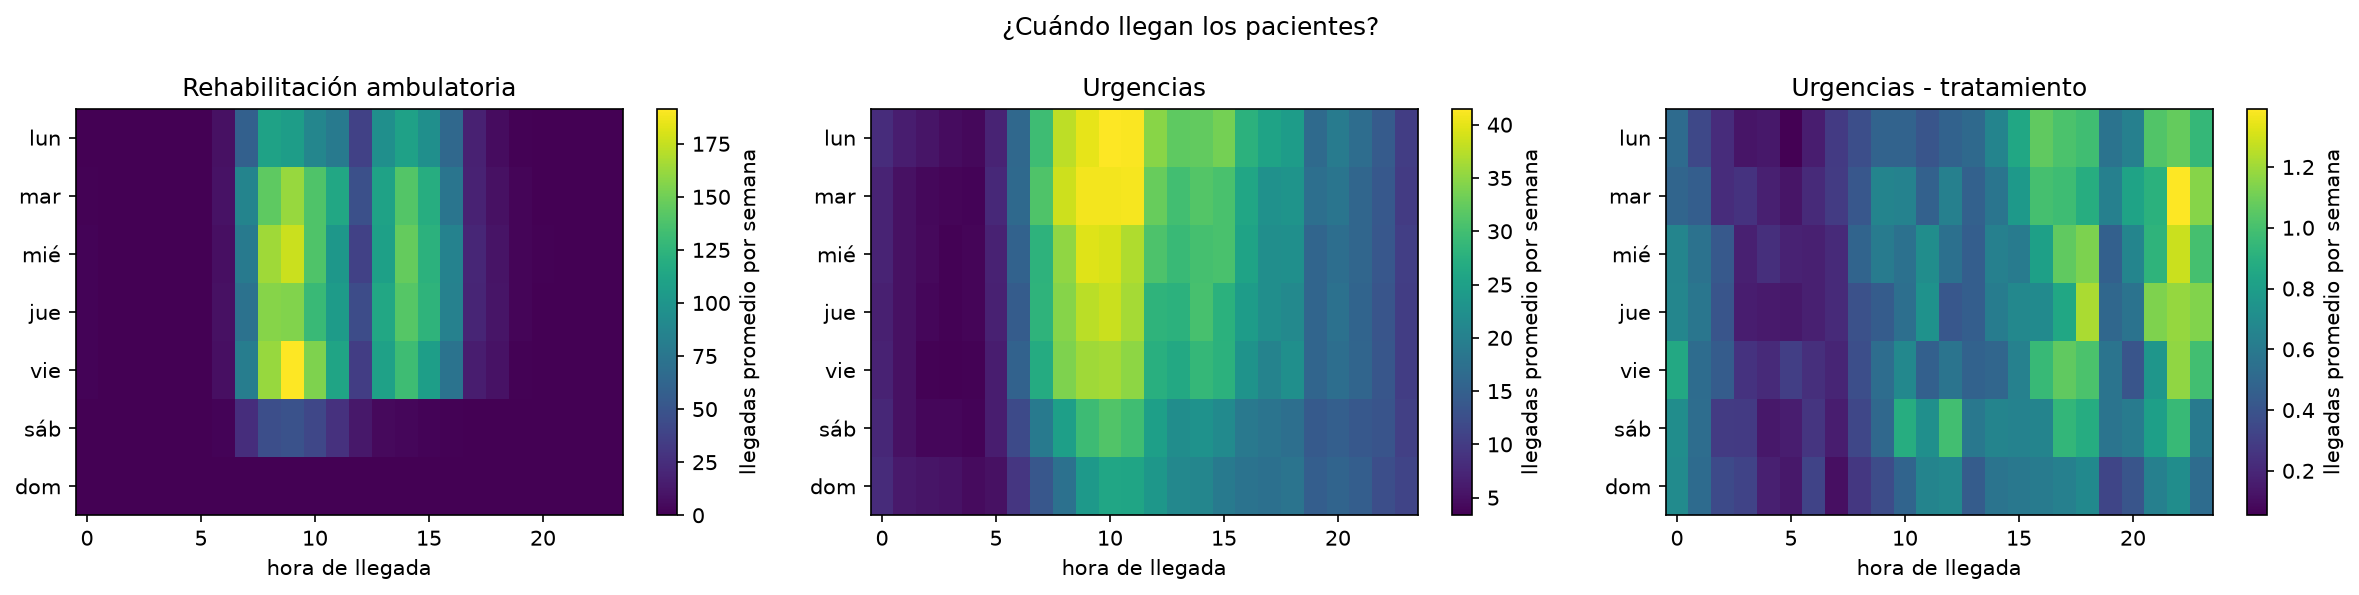
\includegraphics[width=\textwidth]{01_llegadas_dia_hora.png}
\apanota{Figura exploratoria archivada (\texttt{reports/figures/exploracion/01\_llegadas\_dia\_hora.png}). Refleja distribución descriptiva histórica por servicio; no representa una curva de rendimiento predictivo ni debe utilizarse para estimar cifras exactas por lectura visual.}
\end{figure}

\begin{figure}[htbp]
\caption{Tendencia histórica de llegadas diarias en media móvil de 28 días (2023--2026)}
\label{fig:exploracion_tendencia}
\centering
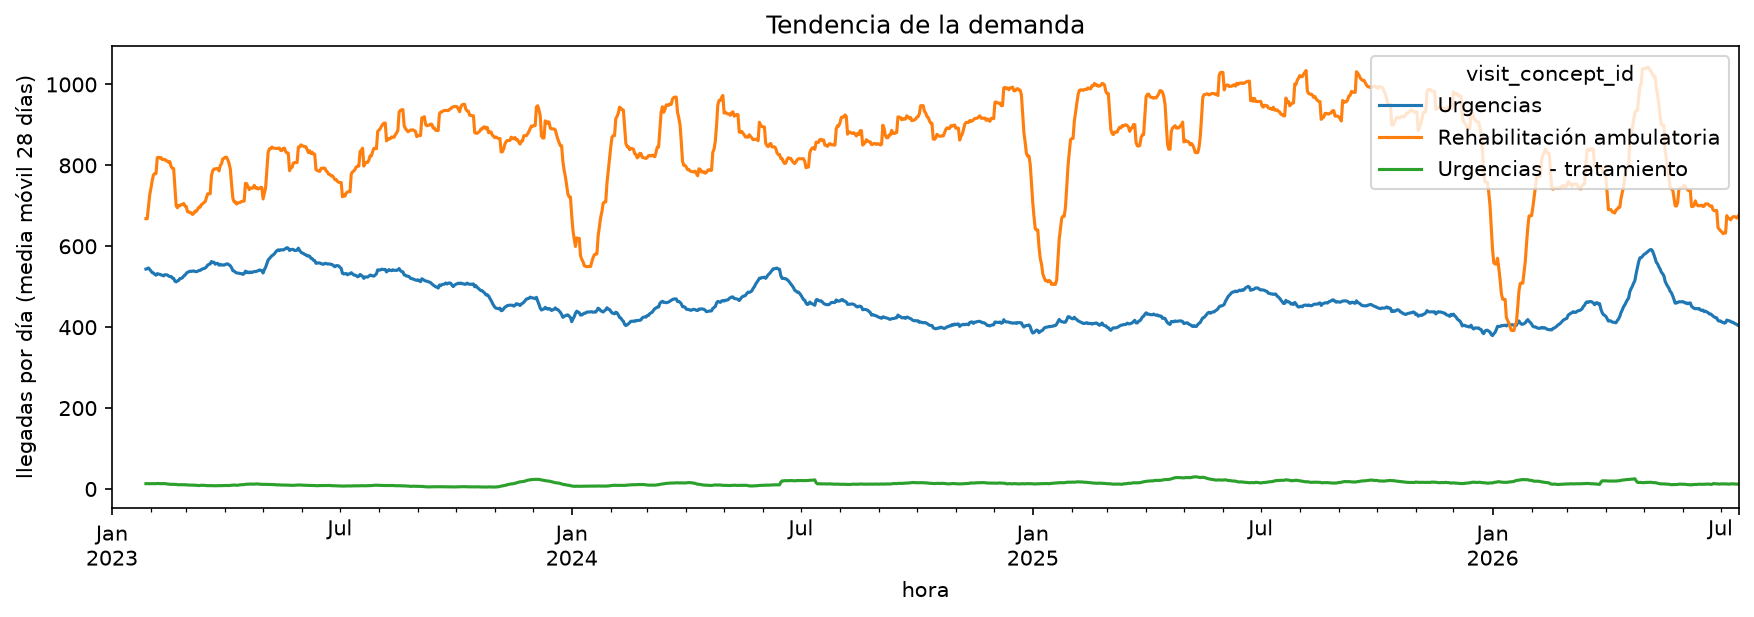
\includegraphics[width=\textwidth]{02_tendencia.png}
\apanota{Figura exploratoria archivada (\texttt{reports/figures/exploracion/02\_tendencia.png}). Muestra la evolución histórica agregada de llegadas y los descensos estacionales de Rehabilitación en Carnaval y cierre de año. No incorpora proyecciones fuera de muestra.}
\end{figure}

\begin{figure}[htbp]
\caption{Duración mediana ($p_{50}$) de etapas según día de la semana y hora de inicio}
\label{fig:exploracion_duracion}
\centering
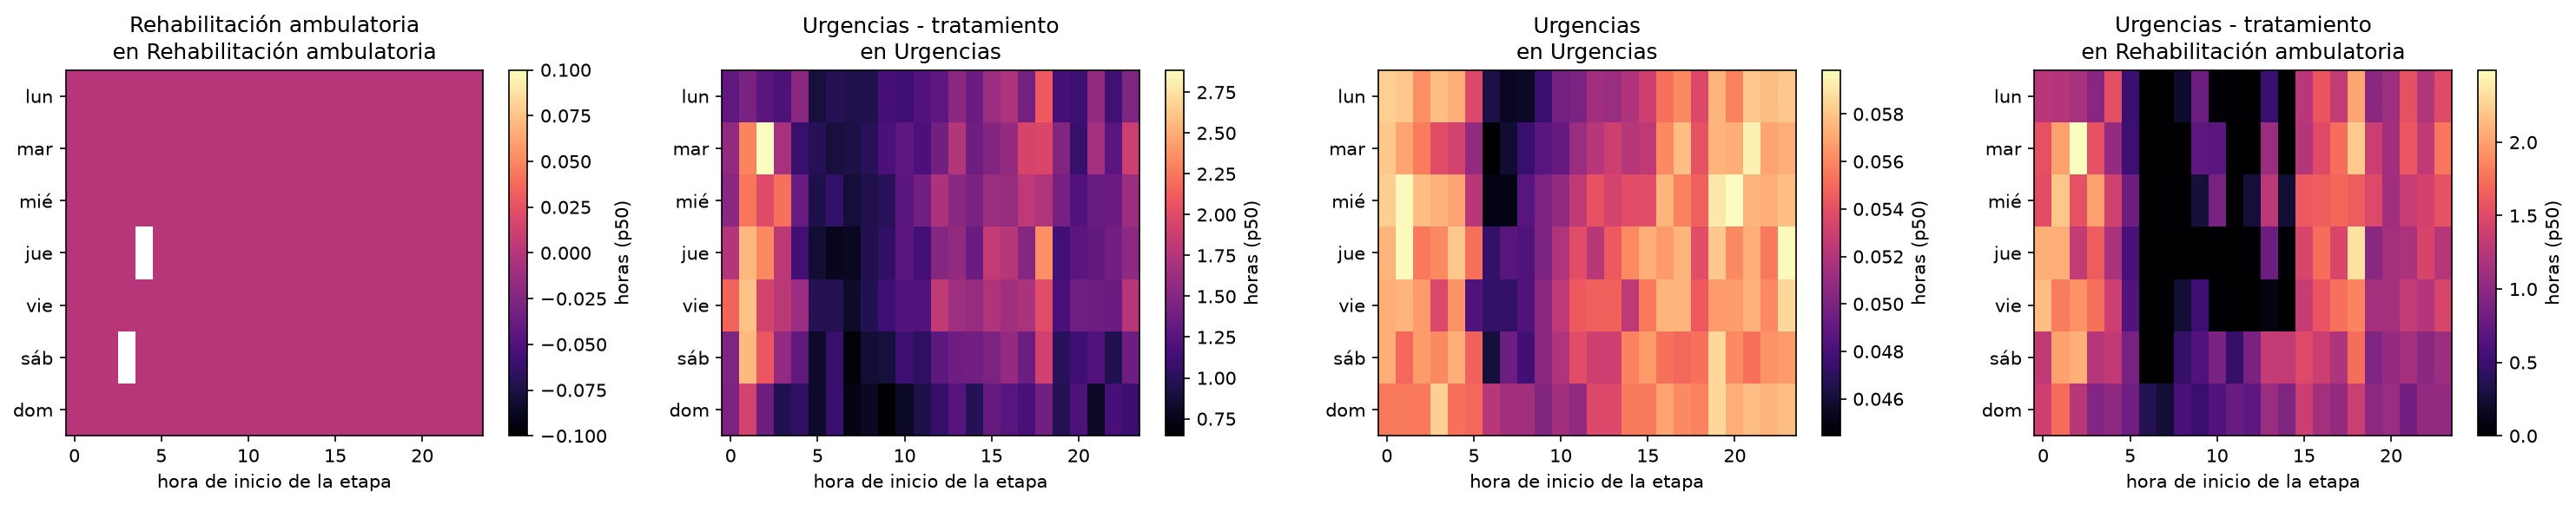
\includegraphics[width=\textwidth]{03_duracion_etapas_franja.png}
\apanota{Figura exploratoria archivada (\texttt{reports/figures/exploracion/03\_duracion\_etapas\_franja.png}). Representa tiempos históricos por franja de inicio en horas; la ausencia de marcas de salida distintas del inicio en Rehabilitación explica los valores nulos en su panel.}
\end{figure}

\subsection{Transición prioritaria entre Tratamiento Urgencias y Hospitalización}

El análisis de pasos secuenciales en \texttt{18\_transiciones\_etapas.sql} identifica como transición prioritaria el salto administrativo desde \textit{Treatment urgency} (\texttt{3045729}) hacia \textit{Inpatient Visit} (\texttt{9201}) dentro de visitas de Urgencias (\texttt{9203}), con \textbf{\num{47670} pasos} acumulados \parencite{mediflow2026optimizacion}. En esta consulta, el indicador de espera entre etapas se define mediante $\text{espera\_h} = \text{inicio\_siguiente} - \text{fin\_anterior}$ sobre etapas con fecha de egreso válida ordenadas por inicio y \texttt{visit\_detail\_id}. En el resumen archivado, el $p_{50}$ mensual ponderado por número de pasos es \num{0,0}\,h y el $p_{90}$ mensual ponderado alcanza \textbf{\num{24,45}\,h} (\num{24,446}\,h sin redondear).

Tres advertencias condicionan la lectura de este indicador. Primero, la definición $\text{inicio\_siguiente} - \text{fin\_anterior}$ admite valores negativos por solapamiento administrativo entre registros, por lo que no equivale a un tiempo clínico de espera por cama asignada ni mide por sí sola episodios de \textit{boarding}. Segundo, el valor \num{24,45}\,h corresponde al promedio de los percentiles $p_{90}$ mensuales ponderado por el volumen mensual de pasos, y no al percentil 90 global calculado sobre los \num{47670} registros individuales agrupados. Tercero, al cruzar mensualmente ese $p_{90}$ con el censo medio mensual de Hospitalización se observa una correlación ecológica negativa de $r = -0{,}481$, con $p_{90}$ ponderado de \num{25,13}\,h en meses de censo normal frente a \num{23,70}\,h en meses de censo alto \parencite{mediflow2026optimizacion}. Este patrón descarta atribuir de forma causal el alargamiento de la transición a la congestión agregada de piso y exige auditar directamente los sellos temporales en el sistema asistencial antes de prometer reducciones de espera por cama mediante redistribución de egresos.

% Sección 3: Calidad, preparación e integración de factores externos
% evidencia:E04,E05,E10,E26

\section{Calidad, preparación e integración de factores externos}

La confiabilidad de los modelos predictivos y de la reconstrucción del censo depende de resolver anomalías estructurales del registro administrativo antes de entrenar o simular. El equipo ejecutó una auditoría SQL de solo conteos sobre las tablas clínicas principales y formalizó reglas de depuración directamente dentro de las consultas de extracción y del preprocesamiento en Python \parencite{mediflow2026calidad,mediflow2026informe}.

\subsection{Auditoría archivada de calidad y consistencia temporal}

Los resultados archivados de la auditoría del 28 de octubre de 2026 \parencite{mediflow2026calidad} documentan completitud total (0,00\,\% de valores nulos) en las columnas clave de \texttt{person} (\num{912205} filas), \texttt{visit\_occurrence} (\num{1706001} filas) y \texttt{visit\_detail} (\num{3281613} filas). Aunque los identificadores primarios (\texttt{visit\_occurrence\_id} y \texttt{visit\_detail\_id}) no presentan repeticiones, el agrupamiento por clave de evento revela duplicidad administrativa significativa en visitas principales y residual en etapas. Adicionalmente, el cruce con el año de nacimiento detectó edades biológicamente imposibles que distorsionaban el grupo pediátrico cuando no se reclasificaban explícitamente.

Para verificar si la anonimización había desplazado artificialmente las fechas respecto del calendario colombiano real, la auditoría midió el volumen relativo de visitas en festivos entre semana frente a las tres semanas vecinas del mismo día de la semana, desplazando la referencia entre $-21$ y $+21$ días \parencite{mediflow2026calidad}. En Rehabilitación Ambulatoria (citas programadas que cierran en días no laborales), el mínimo global se alcanzó exactamente en el desfase de 0 días con un volumen relativo de 0,0032 (0,32\,\%) en \texttt{visit\_occurrence} y 0,0033 (0,33\,\%) en etapas de \texttt{visit\_detail}, con márgenes de 0,50 y 0,49 frente al segundo menor desplazamiento, respectivamente, además de caídas casi totales en lunes y martes de Carnaval (0,25\,\% y 0,21\,\%) y cierre de fin de año. Aunque Urgencias no discrimina por su operación continua 24/7 (73,95\,\% en festivos), la prueba aporta consistencia calendario-registro suficiente para habilitar variables calendáricas reales, sin constituir una certificación absoluta de exactitud para cada marca horaria individual. Todas estas cifras corresponden a resultados archivados del equipo y no a una nueva consulta SQL ejecutada para la edición del presente informe.

\begin{table}[htbp]
\caption{Reglas de calidad de datos, hallazgos archivados e implementación SQL vigente}
\label{tab:reglas_calidad}
{\singlespacing\small
\begin{tabularx}{\textwidth}{@{}L{0.18\textwidth} L{0.30\textwidth} L{0.24\textwidth} Y@{}}
\toprule
Dimensión & Hallazgo archivado y población & Implementación vigente & Efecto o límite \\
\midrule
Nulos críticos & 0,00\,\% en claves y marcas de \texttt{person}, \texttt{visit\_occurrence} y \texttt{visit\_detail} & No requiere imputación de fechas & Validez de completitud condicionada al extracto \\
Duplicados en visitas & \num{228259} copias sobrantes (13,38\,\%) sobre \num{1706001} filas & \texttt{COUNT(DISTINCT (person\_id, concept, inicio))} en SQL \texttt{04}, \texttt{11}, \texttt{13} & Reduce las llegadas totales a \num{1477742} ($-13{,}4\,\%$) \\
Duplicados en etapas & \num{14081} copias sobrantes (0,43\,\%) sobre \num{3281613} etapas & Conteo agregado por etapa; tasa distinta a visitas & No extrapolar 0,43\,\% como tasa de visitas \\
Edades imposibles & 43 visitas (22 pacientes, 0,0025\,\%): edad $<0$ o $>110$ años & Etiqueta \texttt{invalida} en SQL \texttt{10} y \texttt{13} & Evita inflar el grupo pediátrico \texttt{0-17} \\
Etapas inválidas y huérfanas & 0\,\% sin fin o con fin $<$ inicio; 117 huérfanas globales (91 en \texttt{9201}) & SQL \texttt{14}--\texttt{16}, \texttt{18} excluyen fechas inválidas; \texttt{SQL16} usa \texttt{LEFT JOIN} y conserva huérfanas & Ver contraste poblacional en el apartado de recorte $p_{99{,}9}$ \\
Regularización temporal & Ausencia de filas en horas o días sin movimientos & \texttt{grilla\_regular} rellena con 0 en \texttt{agregados.py} & Evita sesgar al alza los promedios horarios y diarios \\
\bottomrule
\end{tabularx}}
\apanota{Síntesis contrastada entre \textcite{mediflow2026calidad}, \textcite{mediflow2026informe} (sección~3) y los archivos SQL \texttt{04}, \texttt{13}, \texttt{14}, \texttt{15}, \texttt{16} y \texttt{18} de \texttt{src/hun/data/sql/}.}
\end{table}

\subsection{Depuración estadística de estancias extremas (\texorpdfstring{$p_{99{,}9}$}{p99.9}) y regla vigente sobre huérfanas}

La auditoría sin recorte ejecutada en \texttt{23\_duracion\_etapas\_percentiles.sql} reveló colas administrativas extremas que distorsionaban la reconstrucción acumulada del censo horario: los máximos crudos alcanzaron \num{28070,3}\,h en Tratamiento Urgencias, \num{20730,3}\,h en Urgencias y \num{11213,6}\,h en Hospitalización \parencite{mediflow2026saturacion,mediflow2026informe}. Para evitar que registros abiertos o anomalías de cierre inflaran artificialmente la ocupación acumulada, las consultas \texttt{14\_etapas\_entradas\_por\_hora.sql}, \texttt{15\_etapas\_salidas\_por\_hora.sql} y \texttt{16\_duracion\_etapas\_diaria.sql} aplican como filtro superior el percentil $p_{99{,}9}$ calculado por cada tipo de etapa sobre duraciones válidas: \textbf{\num{1176,3}\,h} en Hospitalización (\num{1176,257222}\,h exactas), \textbf{\num{283,7}\,h} en Tratamiento Urgencias, \textbf{\num{17,5}\,h} en Urgencias y \textbf{0,0\,h} en Rehabilitación Ambulatoria \parencite{mediflow2026saturacion}.

En Hospitalización (\texttt{9201}), sobre un universo de \num{108601} etapas válidas, exactamente 107 superan el umbral de \num{1176,3}\,h (todas ellas asociadas a visita padre) y quedan excluidas, conservando \textbf{\num{108494} etapas} incluidas las 91 etapas huérfanas (cuya duración individual es inferior a 720\,h) \parencite{mediflow2026informe}. Al aplicar este filtro sobre el censo horario posterior al calentamiento, los percentiles $p_{50}/p_{75}/p_{90}$ de Hospitalización pasan de 288 / 306 / 319 (máximo 378) a \textbf{283 / 297 / 309} (máximo \textbf{359}), mientras los de Tratamiento Urgencias pasan de 219 / 260 / 300 a \textbf{201 / 239 / 272} \parencite{mediflow2026informe}. Este filtro debe interpretarse estrictamente como un recorte estadístico agregado que puede excluir estancias reales prolongadas; no constituye una adjudicación clínica caso a caso.

El contraste directo del código SQL permite resolver una divergencia documental existente en el repositorio. Mientras algunas frases históricas de \textcite{mediflow2026calidad} recomiendan excluir las etapas huérfanas sin registro en \texttt{visit\_occurrence}, la implementación vigente en \texttt{16\_duracion\_etapas\_diaria.sql} utiliza \texttt{LEFT JOIN visit\_occurrence} bajo el mismo criterio de \texttt{SQL14} y \texttt{SQL15}, conservando la población común de \num{108494} etapas. Si se exigiera visita padre mediante unión interna, la cohorte se reduciría a \num{108403} etapas, definiendo una población distinta \parencite{mediflow2026informe}. En este informe prevalece la regla implementada en el SQL vigente para describir la arquitectura actual del censo alineado, conservando el registro de la población alternativa en el análisis de Ley de Little.

\subsection{Integración externa y protocolo de cuatro filtros}

El módulo independiente \texttt{src/external/} genera la tabla diaria de factores externos (\texttt{data/externos.parquet}) integrando calendario colombiano (librería \texttt{holidays} con festivos, puentes y día posterior al festivo, Carnaval de Barranquilla, Semana Santa, vacaciones escolares y quincenas/primas), meteorología histórica de Open-Meteo para las coordenadas de Soledad y series epidemiológicas semanales de SIVIGILA para dengue e infección respiratoria aguda grave con rezagos anti-fuga de dos y tres semanas (\texttt{lag2s} y \texttt{lag3s}). El archivo de control \texttt{data/externos\_fuentes.json} fechado el 27 de octubre de 2026 certifica estado \texttt{ok} para calendario, clima (del \texttt{2018-01-01} al \texttt{2026-10-21}) y epidemiología; sin embargo, la mera disponibilidad de una fuente no acredita aporte predictivo ni completitud diaria en el horizonte operativo \parencite{mediflow2026informe}.

\begin{table}[htbp]
\caption{Resultados archivados del protocolo de evaluación empírica de factores externos}
\label{tab:factores_externos}
{\singlespacing\small
\begin{tabularx}{\textwidth}{@{}L{0.23\textwidth} l r r r r Y@{}}
\toprule
Grupo evaluado & Decisión & Mediana & Placebo & Pliegues & $p$-signo & Motivo registrado \\
\midrule
\texttt{festivos\_y\_puentes} & Acepta & $+33{,}80\,\%$ & $-1{,}80\,\%$ & 88\,\% & 0,000 & Cumple los 4 criterios \\
\texttt{carnaval\_y\_}\allowbreak\texttt{semana\_santa} & Acepta & $+3{,}49\,\%$ & $+1{,}26\,\%$ & 73\,\% & 0,014 & Cumple los 4 criterios \\
\texttt{vacaciones\_}\allowbreak\texttt{escolares} & Descarta & $+4{,}41\,\%$ & $-0{,}13\,\%$ & 65\,\% & 0,084 & $< 70\,\%$ de pliegues y $p > 0{,}05$ \\
\texttt{quincena\_y\_primas} & Descarta & $+1{,}17\,\%$ & $+0{,}79\,\%$ & 58\,\% & 0,279 & Placebo alto ($> 0{,}5\times$), $< 70\,\%$ pliegues y $p > 0{,}05$ \\
\bottomrule
\end{tabularx}}
\apanota{Tomado de \textcite{mediflow2026externos} (corrida del 18 de noviembre de 2026 sobre 26 pliegues \textit{walk-forward}). Los criterios de aceptación exigen mediana de mejora relativa $\ge 1\,\%$, mejora en $\ge 70\,\%$ de pliegues, prueba unilateral de signo con $p \le 0{,}05$ y mejora del placebo desplazado inferior a la mitad de la mejora real. Los grupos \texttt{clima} y \texttt{epidemiologia} fueron descartados en una corrida inicial anterior \parencite{mediflow2026informe}; la tabla vigente del 18 de noviembre no contiene sus métricas numéricas, por lo que no se reproducen ni interpolan valores para dichos grupos. Las cifras de prueba del placebo de festivos en la nota de \texttt{docs/protocolo\_factores\_externos.md} ($+29{,}6\,\%$, placebo $-0{,}69\,\%$) corresponden a una corrida previa a la actualización del 18 de noviembre.}
\end{table}

Para impedir atribuir a variables exógenas mejoras explicables por estacionalidad o azar, el protocolo somete cada grupo en bloque a cuatro pruebas consecutivas sobre los 26 pliegues de validación temporal: ablación contra un modelo base ya dotado de día de la semana, mes y armónicos anuales; control de estacionalidad; prueba placebo desplazando el factor en el tiempo preservando estructura semanal; y estabilidad mediante porcentaje de pliegues mejorados junto con prueba unilateral de signo \parencite{mediflow2026externos}. La Tabla~\ref{tab:factores_externos} resume los resultados de la corrida del 18 de noviembre de 2026: solo los grupos \texttt{festivos\_y\_puentes} (6 variables) y \texttt{carnaval\_y\_semana\_santa} (5 variables) superan todos los umbrales y son aceptados en el diseño de \texttt{lgbm\_final}.

% Sección 4: Metodología analítica y diseño de validación temporal
% evidencia:E08,E09,E11,E12,E13,E14

\section{Metodología analítica y diseño de validación temporal}

El diseño predictivo de MediFlow separa estrictamente tres familias de modelos que cumplen propósitos distintos dentro del sistema: una escalera experimental puntual basada en modelos de conteo (Poisson) para contrastar hipótesis y seleccionar variables externas; un conjunto de modelos cuantílicos servido en la aplicación web para proveer intervalos y descomposiciones explicativas; y un modelo independiente sin rezagos cortos para proyectar horizontes de hasta cuatro meses. Todas las familias comparten la prohibición de particiones aleatorias y se evalúan mediante validación temporal de origen móvil (\textit{walk-forward}) \parencite{hyndman_fpp3}.

\subsection{Validación temporal de origen móvil y política anti-fuga}

Sea $\{y_{s,t}\}$ la serie regular diaria de llegadas únicas del servicio $s$ en la fecha $t$. Para un pliegue $k$ definido por un origen temporal $o_k$ y un horizonte $h$, la partición temporal en \texttt{src/hun/models/validacion.py} impone:
\begin{equation}
\label{eq:walk_forward}
\mathcal{D}_{\text{train}}^{(k)} = \{(s, t) : t < o_k\}, \qquad
\mathcal{D}_{\text{test}}^{(k)} = \{(s, t) : o_k \le t < o_k + h\},
\end{equation}
de modo que ningún registro de entrenamiento incluye fechas iguales o posteriores al origen del pliegue. En la evaluación operativa a corto plazo se utilizan \textbf{26 pliegues} con orígenes comprendidos entre \texttt{2025-07-25} y \texttt{2026-07-10}, paso fijo de 14 días y horizonte $h = 7$ días \parencite{mediflow2026demanda}. Debido a que el paso de 14 días es múltiplo de siete, todos los orígenes caen en viernes; en consecuencia, el día 1 del horizonte corresponde siempre a viernes, el día 2 a sábado, el día 3 a domingo y así sucesivamente hasta el jueves. El día del horizonte y el día de la semana quedan estructuralmente confundidos, por lo que las variaciones de error entre los días 1 y 7 no deben atribuirse únicamente al alejamiento temporal del pronóstico. En el horizonte extendido de largo plazo se emplean \textbf{13 pliegues} entre \texttt{2025-03-24} y \texttt{2026-03-19} con paso de 30 días y horizonte $h = 120$ días; como el horizonte cuadruplica el paso, las ventanas de prueba consecutivas se solapan extensamente y no constituyen muestras independientes \parencite{mediflow2026largoplazo}.

La política anti-fuga implementada en \texttt{construir\_features\_demanda} de \texttt{src/hun/models/demanda.py} enmascara explícitamente el vector objetivo $y_{s,t}$ como faltante para todo $t \ge o_k$ antes de calcular desplazamientos semanales (\texttt{llegadas\_lag\_7} hasta \texttt{llegadas\_lag\_56}, además de \texttt{rezago\_prom\_4s} y \texttt{rezago\_mediana\_8s}). Así, para predecir cualquier día dentro de $[o_k, o_k + 7\,\text{d})$, los rezagos mínimos de siete días consultan exclusivamente observaciones estrictamente anteriores al origen. Las series epidemiológicas de SIVIGILA incorporan rezagos de dos y tres semanas y el modelo de largo plazo sustituye cualquier observación meteorológica posterior por medianas climáticas por día del año calculadas con fechas anteriores a cada corte. Como límite explícito, este mecanismo protege la evaluación \textit{walk-forward} de 1--7 días, pero no hereda automáticamente esa garantía cuando la aplicación web realiza inferencia puntual en fechas posteriores al corte usando medianas históricas de respaldo (\texttt{medianas\_dw}) ni cuando el modelo final entrenado con toda la historia se consulta sobre fechas ya vistas \parencite{mediflow2026bundle,mediflow2026informe}.

\subsection{Métricas de evaluación y techo Poisson idealizado}

Dado que las series hospitalarias exhiben días con volumen nulo o muy bajo (por ejemplo, Rehabilitación en domingos), las métricas basadas en porcentajes individuales como MAPE divergen. Siguiendo la decisión técnica \texttt{DEC-003}, la evaluación adopta el Error Porcentual Absoluto Ponderado (WAPE), acompañado de MAE, RMSE, sesgo y cobertura empírica:
{\singlespacing
\begin{equation}
\label{eq:metricas}
\begin{aligned}
\text{WAPE} &= \frac{\sum_{i=1}^{n} |y_i - \hat{y}_i|}{\sum_{i=1}^{n} |y_i|}, &
\text{Exactitud} &= 1 - \text{WAPE}, \\
\text{MAE} &= \frac{1}{n}\sum_{i=1}^{n} |y_i - \hat{y}_i|, &
\text{RMSE} &= \sqrt{\frac{1}{n}\sum_{i=1}^{n} (y_i - \hat{y}_i)^2}, \\
\text{Sesgo} &= \frac{1}{n}\sum_{i=1}^{n} (\hat{y}_i - y_i), &
\text{Cobertura} &= \frac{1}{n}\sum_{i=1}^{n} \mathbf{1}\!\left\{\hat{q}_{0{,}10,i} \le y_i \le \hat{q}_{0{,}90,i}\right\}.
\end{aligned}
\end{equation}
}
En este proyecto, «exactitud» significa estrictamente $1 - \text{WAPE}$ y no porcentaje de días acertados individualmente; un sesgo positivo indica sobreestimación promedio y la meta interna de 80\,\% es un criterio interno de trabajo del equipo, no un umbral de la rúbrica oficial \parencite{mediflow2026demanda,hun2026terminos}. La serie residual \texttt{Otros} (menos de una llegada diaria) se excluye de las métricas globales para no distorsionar los promedios agregados.

Para contextualizar servicios de bajo volumen como Tratamiento Urgencias ($\approx 15{,}2$ llegadas/día), \texttt{techo\_exactitud\_poisson} calcula un techo idealizado suponiendo conteos independientes $X \sim \text{Poisson}(\mu)$ con tasa verdadera conocida $\mu = \bar{y}\cdot d$ ($d=1$ diario, $d=7$ semanal):
\begin{equation}
\label{eq:techo_poisson}
\text{Techo}(\mu) = 1 - \frac{\mathbb{E}\bigl[|X - \mu|\bigr]}{\mu}.
\end{equation}
Puesto que el cálculo presupone conocer la tasa verdadera exacta y que la única fuente de variabilidad es el ruido puro de Poisson sin cambios semanales de nivel, este techo constituye una referencia teórica optimista y no una cota estadística universal \parencite{mediflow2026demanda}.

\subsection{Familia experimental puntual (escalera Poisson y LightGBM)}

La escalera experimental implementada en \texttt{src/hun/models/demanda.py} compara cuatro escalones sobre los mismos 26 pliegues: (1) \texttt{linea\_base}, definida como la mediana del mismo día de la semana durante las últimas ocho semanas; (2) \texttt{poisson\_calendario}, regresión lineal generalizada con enlace logarítmico (\texttt{PoissonRegressor}, $\alpha = 10^{-4}$) ajustada \textbf{de forma estratificada por servicio} (evitando mezclar los cierres festivos de Rehabilitación con la operación 24/7 de Urgencias); (3) \texttt{lgbm\_todos\_externos}, basada en LightGBM \parencite{ke2017lightgbm} con pérdida Poisson (\texttt{n\_estimators=200}, \texttt{learning\_rate=0.05}, \texttt{num\_leaves=15}, \texttt{min\_child\_samples=15}); y (4) \texttt{lgbm\_final}, que restringe las variables externas a los grupos aprobados por el protocolo.

Dos componentes algorítmicos distinguen a los modelos LightGBM de la escalera puntual frente a una configuración genérica. Primero, la ponderación exponencial por recencia asigna a cada fila de entrenamiento un peso $w_i = 0{,}5^{\text{edad}_i / 180}$ (vida media de 180 días). Segundo, la función \texttt{ajustar\_predecir\_lgbm\_nivel} introduce una corrección de nivel local mediante \texttt{init\_score} $= \log(\tilde{y}_{\text{local}})$, donde $\tilde{y}_{\text{local}} = \max(\text{rezago\_mediana\_8s},\, 0{,}5)$, de manera que los árboles predicen en escala logarítmica el factor multiplicativo sobre el nivel reciente de cada servicio y escalan proporcionalmente ante cambios de régimen.

\subsection{Familia cuantílica servida en la aplicación web}

El paquete desplegado para la API web (\texttt{models/modelos\_web\_bundle.joblib}, versión \texttt{2.0}) no sirve el modelo \texttt{lgbm\_final} con pérdida Poisson ni comparte idéntica arquitectura de entrenamiento. En su lugar, \texttt{src/hun/models/explicacion.py} ajusta tres regresores LightGBM independientes mediante pérdida \textit{pinball} o de regresión cuantílica \parencite{koenker1978quantiles,ke2017lightgbm} para los niveles $\tau \in \{0{,}10,\, 0{,}50,\, 0{,}90\}$:
\begin{equation}
\label{eq:pinball}
\rho_\tau(u) = u\bigl(\tau - \mathbf{1}\{u < 0\}\bigr), \qquad u = y - \hat{q}_\tau(x).
\end{equation}
Para evitar cruces entre cuantiles estimados por árboles separados y valores negativos de conteo, se aplica un ordenamiento monotónico y truncamiento posterior:
\begin{equation}
\label{eq:orden_cuantiles}
\bigl(\tilde{q}_{0{,}10},\, \tilde{q}_{0{,}50},\, \tilde{q}_{0{,}90}\bigr) = \max\!\Bigl(0,\; \operatorname{sort}\bigl(\hat{q}_{0{,}10},\, \hat{q}_{0{,}50},\, \hat{q}_{0{,}90}\bigr)\Bigr).
\end{equation}
Este ajuste garantiza coherencia ordinal en las respuestas de la interfaz, pero no certifica ni corrige la calibración probabilística de la cobertura empírica. Para interpretar las salidas, el modelo mediano $\hat{q}_{0{,}50}$ se descompone mediante valores SHAP exactos de árboles (\texttt{TreeExplainer}) \parencite{lundberg2017shap}, expresados como suma aditiva respecto de un valor base $\phi_0$:
\begin{equation}
\label{eq:shap}
f(x) = \phi_0 + \sum_{j=1}^{M} \phi_j(x),
\end{equation}
agrupando las contribuciones en factores legibles para la interfaz. Las atribuciones SHAP describen contribuciones marginales al pronóstico del modelo y no miden efectos causales de intervenciones operativas.

La inspección directa del código y de la lista de columnas \texttt{cols} almacenada en el artefacto \texttt{v2.0} confirma además dos diferencias estructurales frente a \texttt{lgbm\_final}: la función \texttt{entrenar\_modelos\_cuantiles} no emplea desplazamiento logarítmico de nivel local (\texttt{init\_score}) ni pesos exponenciales por recencia, y las 21 columnas efectivamente empaquetadas en el bundle vigente incluyen 5 variables de calendario, 10 variables de rezago y únicamente las 6 variables de \texttt{festivos\_y\_puentes}, omitiendo las 5 variables de \texttt{carnaval\_y\_semana\_santa} \parencite{mediflow2026bundle}. Por ello, sus métricas de desempeño deben reportarse de forma completamente separada del experimento Poisson.

\subsection{Modelo independiente de horizonte extendido}

Para proyectar de agosto a noviembre de 2026 más allá de los últimos rezagos semanales disponibles en la base (\texttt{2026-07-16}), el módulo \texttt{src/hun/models/largo\_plazo.py} entrena un modelo independiente basado en LightGBM Poisson con decaimiento exponencial por recencia (vida media de 180 días, \texttt{min\_child\_samples=20}) sin ningún rezago corto de llegadas. Sus predictores combinan 7 variables de calendario, 6 de \texttt{festivos\_y\_puentes}, la tendencia secular \texttt{tendencia\_anios}, el identificador de servicio y las medianas climáticas históricas por día del año calculadas estrictamente con fechas anteriores a cada corte. Para contener el deterioro de incertidumbre entre uno y cuatro meses, los intervalos parten de regresores cuantílicos base en $p_{05}$ y $p_{95}$ (\texttt{CUANTIL\_BAJO = 0,05} y \texttt{CUANTIL\_ALTO = 0,95}) expandidos alrededor de la estimación puntual $\hat{y}$ según el mes del horizonte $m \in \{1,2,3,4\}$ mediante el factor $1 + 0{,}10\,(m - 1)$, aunque el esquema JSON expuesto a la interfaz rotule los extremos resultantes como \texttt{min\_diario}/\texttt{max\_diario} o intervalo $[p_{10}, p_{90}]$ \parencite{mediflow2026largoplazo}.

% Sección 5: Resultados predictivos por familia de evidencia
% evidencia:E08,E09,E12,E13,E14

\section{Resultados predictivos por familia de evidencia}

Siguiendo la separación metodológica establecida en la sección anterior, los resultados predictivos se presentan en tres bloques independientes: la corrida experimental puntual de demanda del 18 de noviembre de 2026, los metadatos archivados del artefacto cuantílico servido en la web (\texttt{v2.0}) en contraste con el reporte histórico de intervalos del 3 de noviembre, y las dos corridas comprobadas para el horizonte extendido a 120 días.

\subsection{Experimento puntual Poisson: escalera, servicios, festivos y estabilidad}

En los 26 pliegues \textit{walk-forward} del experimento puntual reportado el 18 de noviembre de 2026 \parencite{mediflow2026demanda}, la incorporación progresiva de estructura estratificada por servicio, nivel local con pesos por recencia y factores externos validados reduce el error global de manera consistente. La Tabla~\ref{tab:escalera_poisson} recoge las métricas globales de la escalera sin incluir la serie residual \texttt{Otros}.

\begin{table}[htbp]
\caption{Escalera predictiva puntual en 26 pliegues \textit{walk-forward} (experimento del 18 de noviembre de 2026)}
\label{tab:escalera_poisson}
{\singlespacing\small
\begin{tabularx}{\textwidth}{@{}Y r r r r r@{}}
\toprule
Modelo evaluado & WAPE & MAE & RMSE & Sesgo & Mejora rel. \\
\midrule
1. Línea base (mediana de 8 semanas) & 18,0\,\% & 77,02 & 201,34 & $+21{,}44$ & Referencia \\
2. Poisson estratificado por servicio & 15,6\,\% & 66,86 & 125,91 & $+6{,}41$ & $+13{,}2\,\%$ \\
3. LightGBM nivel local (todos externos) & 10,5\,\% & 44,84 & 83,82 & $-6{,}00$ & $+41{,}8\,\%$ \\
4. LightGBM Poisson final (\texttt{lgbm\_final}) & 10,5\,\% & 44,94 & 83,67 & $-5{,}70$ & $+41{,}6\,\%$ \\
\bottomrule
\end{tabularx}}
\apanota{Datos archivados de \textcite{mediflow2026demanda}, sección~1 (orígenes \texttt{2025-07-25} a \texttt{2026-07-10}, horizonte 1--7 días). Las mejoras relativas frente a la línea base fueron calculadas con las cifras sin redondear antes de su publicación, por lo que no deben recalcularse a partir de 18,0\,\% y 10,5\,\% redondeados. El modelo \texttt{lgbm\_final} conserva únicamente los grupos aceptados (\texttt{festivos\_y\_puentes} y \texttt{carnaval\_y\_semana\_santa}) y se selecciona por parsimonia y respaldo empírico, aunque los dos escalones LightGBM coincidan en WAPE a una decimal.}
\end{table}

El desempeño desagregado del modelo seleccionado \texttt{lgbm\_final} evidencia una fuerte heterogeneidad entre servicios (Tabla~\ref{tab:servicios_poisson}). En Urgencias (\texttt{9203}) y Rehabilitación Ambulatoria (\texttt{581479}), el error WAPE global es de 8,4\,\% y 11,0\,\% (exactitudes $1-\text{WAPE}$ de 91,6\,\% y 89,0\,\%, respectivamente). Sin embargo, el detalle por día de la semana confirma que en Rehabilitación la exactitud cae a 51,3\,\% los sábados (media de 87,1 llegadas/día) y a 15,6\,\% los domingos (media de 2,2 llegadas/día), frente a valores de 85,6\,\% a 90,9\,\% entre lunes y viernes (835,7 a 1.306,2 llegadas/día) \parencite{mediflow2026demanda}. En Tratamiento Urgencias (\texttt{3045729}), con una media de 15,17 llegadas/día, el WAPE diario alcanza 43,5\,\% (exactitud 56,5\,\%, MAE 6,59 pacientes). Contrastado contra el techo idealizado de Poisson, el modelo alcanza 56,5\,\% diario frente a un techo de 79,5\,\%, y al agregar la semana completa en los 26 pliegues alcanza 77,0\,\% frente a un techo semanal de 92,3\,\% \parencite{mediflow2026demanda}. Dado que permanece por debajo de ambas cotas optimistas, el error de este servicio obedece tanto a la varianza de conteos bajos como a cambios semanales en su tasa subyacente, por lo que no debe declararse cumplida la meta operativa diaria.

\begin{table}[htbp]
\caption{Desempeño por servicio del experimento puntual \texttt{lgbm\_final}}
\label{tab:servicios_poisson}
{\singlespacing\small
\begin{tabularx}{\textwidth}{@{}Y r r r r r@{}}
\toprule
Servicio & WAPE & $1-\text{WAPE}$ & MAE & Sesgo & Prom. real \\
\midrule
Emergency Room Visit (\texttt{9203}) & 8,4\,\% & 91,6\,\% & 37,02 & $-7{,}83$ & 443,16 \\
Ambulatory Rehab. (\texttt{581479}) & 11,0\,\% & 89,0\,\% & 91,22 & $-10{,}12$ & 826,54 \\
Treatment urgency (\texttt{3045729}) & 43,5\,\% & 56,5\,\% & 6,59 & $+0{,}86$ & 15,17 \\
\bottomrule
\end{tabularx}}
\apanota{Datos archivados de \textcite{mediflow2026demanda}, sección~2 (26 pliegues, 182 días por servicio, excluyendo \texttt{Otros}). Estas métricas pertenecen al experimento LightGBM Poisson y no deben transferirse al modelo cuantílico servido en la aplicación web.}
\end{table}

Al comparar días normales frente a días festivos \parencite{mediflow2026demanda}, en días normales el WAPE desciende de 12,4\,\% en la línea base (MAE 55,63; sesgo $-3{,}45$) a 10,3\,\% en \texttt{lgbm\_final} (MAE 45,97; sesgo $-6{,}96$), mientras que en días festivos la línea base exhibe WAPE de 317,8\,\% (MAE 409,64; sesgo $+408{,}36$) debido a la sobreestimación masiva cuando Rehabilitación cierra casi por completo, frente a 22,5\,\% en \texttt{lgbm\_final} (MAE 29,03; sesgo $+13{,}89$). Este contraste refleja el efecto mecánico de dividir por un volumen festivo muy bajo en la métrica base y la captura calendárica del modelo, no un impacto causal sobre la demanda hospitalaria. A lo largo del horizonte 1--7 días, el WAPE agregado oscila entre 9,4\,\% (día 7, jueves) y 17,0\,\% (día 2, sábado); entre pliegues individuales, oscila entre 5,4\,\% (pliegue 17, \texttt{2026-03-20}) y 28,0\,\% en el pliegue 11 (\texttt{2025-12-26}, fin de año, donde la línea base alcanza 137,9\,\%) y 27,6\,\% en el pliegue 19 (\texttt{2026-04-17}) \parencite{mediflow2026demanda}. Las series completas de los 26 pliegues y la matriz por servicio y día se conservan en el Anexo~B.

\subsection{Artefacto cuantílico servido en la aplicación web (\texttt{v2.0})}

Los metadatos efectivamente empaquetados en \texttt{models/modelos\_web\_bundle.joblib} (inspeccionados directamente sin reejecutar entrenamientos ni consultas a base de datos) muestran el rendimiento fuera de muestra sobre 182 días (\texttt{2025-07-25} a \texttt{2026-07-16}) de la variante cuantílica $p_{10}/p_{50}/p_{90}$ consumida por la API web. La Tabla~\ref{tab:bundle_cuantilico} expone sus métricas separadas de la Tabla~\ref{tab:servicios_poisson}. En Urgencias el WAPE de $p_{50}$ es 8,91\,\% (frente a 8,4\,\% del experimento Poisson), en Rehabilitación 11,08\,\% y en Tratamiento Urgencias 42,18\,\%. La cobertura empírica $p_{10}$--$p_{90}$ almacenada asciende a 78,57\,\% en Urgencias, 64,29\,\% en Rehabilitación y 73,08\,\% en Tratamiento Urgencias, quedando por debajo del objetivo nominal de 80\,\%, especialmente en Rehabilitación donde los cierres bruscos y la ausencia de nivel local multiplicativo estrechan o desalinean las bandas.

\begin{table}[htbp]
\caption{Métricas archivadas del modelo cuantílico servido en el artefacto web \texttt{v2.0}}
\label{tab:bundle_cuantilico}
{\singlespacing\small
\begin{tabularx}{\textwidth}{@{}Y r r r r r r@{}}
\toprule
Servicio en bundle \texttt{v2.0} & WAPE & MAE & RMSE & Sesgo & Cob. $p_{10}$--$p_{90}$ & Exact. sem. \\
\midrule
Urgencias (\texttt{9203}) & 8,91\,\% & 39,50 & 53,82 & $-2{,}69$ & 78,57\,\% & 94,75\,\% \\
Rehabilitación (\texttt{581479}) & 11,08\,\% & 91,55 & 137,57 & $+4{,}22$ & 64,29\,\% & 91,63\,\% \\
Tratamiento Urg. (\texttt{3045729}) & 42,18\,\% & 6,40 & 8,47 & $-0{,}64$ & 73,08\,\% & 76,60\,\% \\
\bottomrule
\end{tabularx}}
\apanota{Metadatos almacenados en \texttt{comparacion\_real} de \texttt{models/modelos\_web\_bundle.joblib} \parencite{mediflow2026bundle} sobre 182 días (\texttt{2025-07-25} a \texttt{2026-07-16}, corte exclusivo \texttt{2026-07-17}), consultables también vía \texttt{GET /api/modelo}. Las métricas de cobertura fueron calculadas antes de redondear los puntos servidos a enteros; recomputar sobre salidas enteras puede modificar ligeramente la cobertura observada. Techos Poisson almacenados: Urgencias 96,21\,\% diario / 98,57\,\% semanal; Rehabilitación 97,22\,\% / 98,95\,\%; Tratamiento Urgencias 79,53\,\% / 92,26\,\%.}
\end{table}

Resulta indispensable distinguir estas cifras de la corrida histórica archivada en \textcite{mediflow2026intervalos} del 3 de noviembre de 2026. En aquel reporte anterior se documentó una cobertura global de 83,2\,\% (85,2\,\% en Urgencias, 72,0\,\% en Rehabilitación, 75,8\,\% en Tratamiento Urgencias y 100,0\,\% en \texttt{Otros}, con amplitud media de 112,6 pacientes). Al incluir la categoría \texttt{Otros} (donde la cobertura alcanza 100\,\% por volumen casi nulo) y pertenecer a una versión anterior previa a la actualización del 18--19 de noviembre, esa cifra de 83,2\,\% no valida ni representa la calibración del bundle \texttt{v2.0} actual. Adicionalmente, cuando la aplicación web consulta fechas futuras o sin rezagos observados, \texttt{predict.py} sustituye los rezagos faltantes por medianas históricas de día de la semana (\texttt{medianas\_dw}), comportamiento que no hereda la validación de 1--7 días.

La Figura~\ref{fig:resumen_escalera} resume visualmente la distancia metodológica entre la escalera predictiva puntual de esta sección y la simulación histórica de altas tempranas abordada en optimización.

\begin{figure}[htbp]
\caption{Síntesis comparativa entre evaluación predictiva puntual y simulación histórica de altas}
\label{fig:resumen_escalera}
\centering
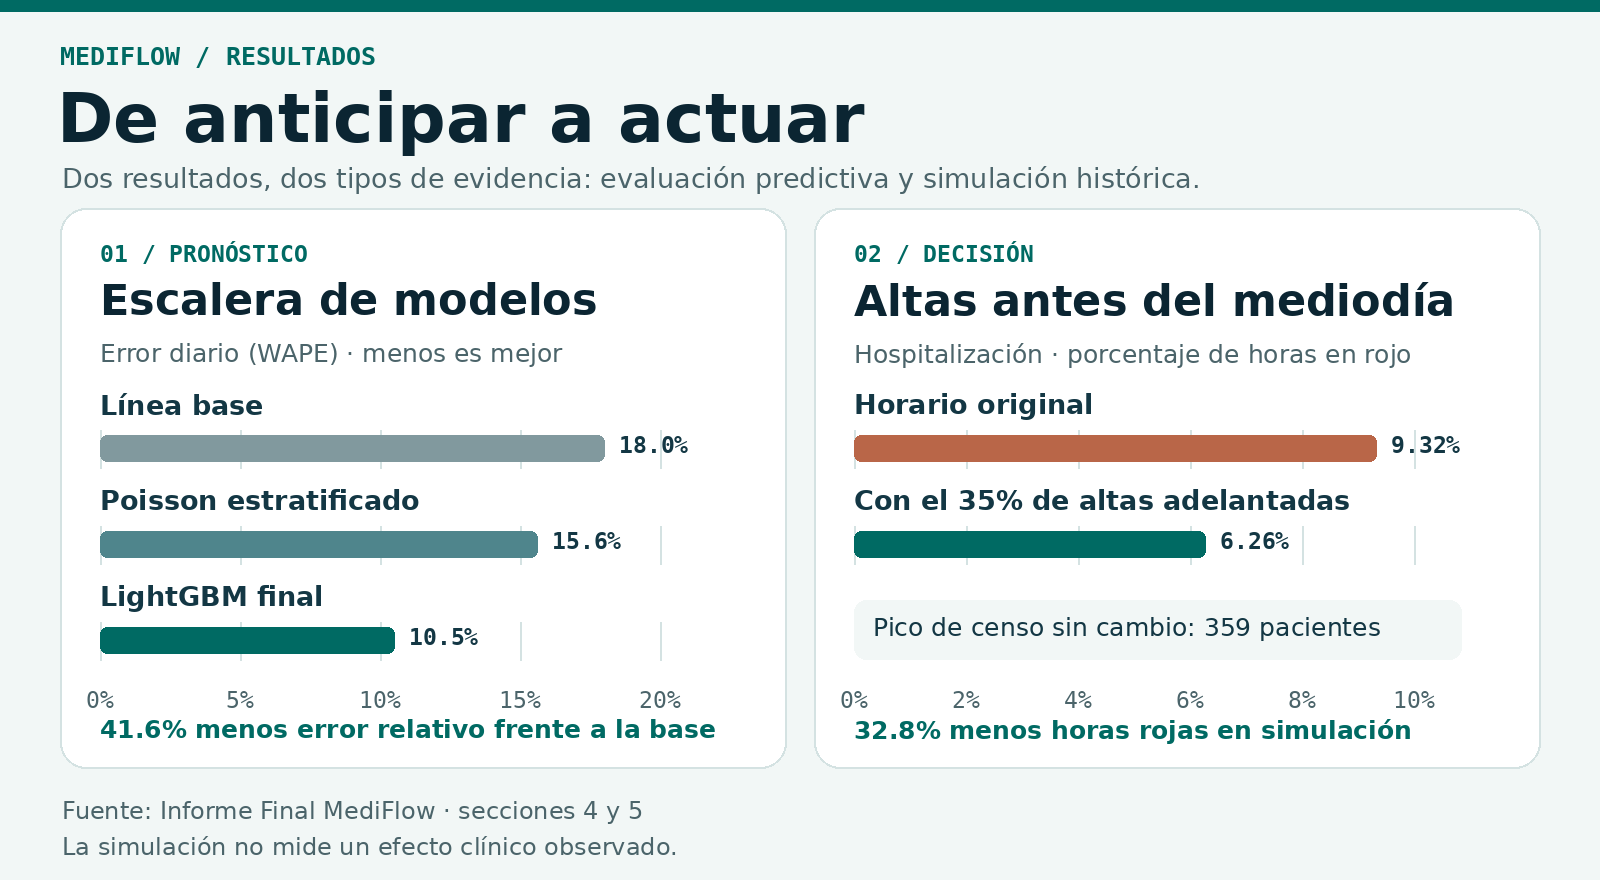
\includegraphics[width=0.92\textwidth]{resumen_escalera_optimizacion.png}
\apanota{Gráfico archivado (\texttt{docs/img/resumen\_escalera\_optimizacion.png}). Los dos paneles representan familias de evidencia independientes: el panel izquierdo corresponde al experimento puntual Poisson en 26 pliegues (WAPE 18,0\,\% $\rightarrow$ 15,6\,\% $\rightarrow$ 10,5\,\%, no al modelo cuantílico web), mientras el panel derecho muestra la simulación histórica determinista de adelanto del 35\,\% de altas en Hospitalización (no un ensayo clínico observado).}
\end{figure}

\subsection{Horizonte extendido a cuatro meses: reporte histórico frente a corrida empaquetada}

Durante el contraste documental contra los artefactos del repositorio se identificó una divergencia relevante entre el reporte Markdown archivado el 3 de noviembre de 2026 \parencite{mediflow2026largoplazo} y la corrida de largo plazo efectivamente empaquetada en el campo \texttt{largo\_plazo} de \texttt{models/modelos\_web\_bundle.joblib} \parencite{mediflow2026bundle} servida por \texttt{GET /api/largo-plazo/\{servicio\}}. Conforme a la decisión editorial aprobada, la Tabla~\ref{tab:largo_plazo_comparado} reporta ambas evidencias por separado sin mezclar sus cifras.

\begin{table}[htbp]
\caption{Desempeño del modelo de largo plazo (120 días, 13 pliegues): reporte archivado frente a bundle servido}
\label{tab:largo_plazo_comparado}
{\singlespacing\small
\begin{tabularx}{\textwidth}{@{}L{0.24\textwidth} Y r r r r r@{}}
\toprule
Fuente y corrida & Servicio & WAPE & $1-\text{WAPE}$ & MAE & Sesgo & Cobertura \\
\midrule
Reporte archivado & Global (sin \texttt{Otros}) & 15,7\,\% & 84,3\,\% & 57,9 & --- & 86,5\,\% \\
(\texttt{2026-11-03}) & Urgencias (\texttt{9203}) & 14,0\,\% & 86,0\,\% & 52,3 & $+20{,}1$ & 85,4\,\% \\
 & Rehabilitación (\texttt{581479}) & 15,5\,\% & 84,5\,\% & 111,7 & $+44{,}2$ & 85,3\,\% \\
 & Tratamiento (\texttt{3045729}) & 64,4\,\% & 35,6\,\% & 9,8 & $+4{,}9$ & 88,7\,\% \\
\midrule
Bundle servido \texttt{v2.0} & Urgencias (\texttt{9203}) & 11,63\,\% & 88,4\,\% & 51,8 & $-15{,}1$ & 87,18\,\% \\
(inspección \texttt{2026-11-19}) & Rehabilitación (\texttt{581479}) & 14,33\,\% & 85,7\,\% & 122,7 & $-2{,}9$ & 83,40\,\% \\
 & Tratamiento (\texttt{3045729}) & 58,12\,\% & 41,9\,\% & 10,1 & $+3{,}9$ & 88,65\,\% \\
\bottomrule
\end{tabularx}}
\apanota{Comparación de dos corridas independientes sobre 13 pliegues solapados (\texttt{2025-03-24} a \texttt{2026-03-19}). La parte superior proviene de \textcite{mediflow2026largoplazo} (donde el WAPE global pasa de 12,2\,\% en el mes 1 a 13,4\,\%, 16,5\,\% y 21,3\,\% en el mes 4, y las proyecciones mensuales agosto--noviembre de 2026 promedian 215,7--221,0 pac./día en Urgencias y 330,5--385,9 en Rehabilitación). La parte inferior proviene de los metadatos inspeccionados en \textcite{mediflow2026bundle} (donde Rehabilitación registra cobertura 77,69\,\% en el mes 1 y 81,79\,\%--87,95\,\% en los meses 2--4, y las proyecciones mensuales promedian 415,6--433,2 pac./día en Urgencias, 661,5--789,6 en Rehabilitación y 15,6--16,1 en Tratamiento). Las proyecciones agosto--noviembre son extrapolaciones desde el corte de julio de 2026 y no corresponden a demanda real observada ni a reentrenamiento con datos de noviembre.}
\end{table}

En el reporte histórico del 3 de noviembre \parencite{mediflow2026largoplazo}, el desempeño agregado cae progresivamente desde 87,8\,\% de exactitud en el mes 1 (WAPE 12,2\,\%) hasta 78,7\,\% en el mes 4 (WAPE 21,3\,\%, ancho medio de banda 424,5 pacientes), y al agregar por semana el servicio de Tratamiento Urgencias alcanza 50,7\,\% de exactitud (WAPE 49,3\,\%). En la corrida empaquetada del bundle \texttt{v2.0}, las tres series muestran menor WAPE en el backtest y proyecciones agosto--noviembre coherentes con los niveles recientes de mediados de 2026 (frente a los promedios notablemente más bajos de la corrida del 3 de noviembre, cuyo origen obedece posiblemente a diferencias previas en el corte o depuración de la serie antes de la actualización de los parquets de entrada), si bien Rehabilitación cae ligeramente por debajo de 80\,\% de cobertura en el primer mes del horizonte (77,69\,\%). El desglose mensual completo de ambas corridas se incluye en el Anexo~B.

% Sección 6: Optimización operacional y simulaciones paramétricas
% evidencia:E15,E16,E17,E18,E19,E20

\section{Optimización operacional y simulaciones paramétricas}

La capa de decisión de MediFlow combina tres modelos analíticos orientados a explorar requerimientos paramétricos de atención, balance promedio de ocupación hospitalaria y redistribución horaria de egresos: teoría de colas M/M/$c$ (Erlang~C), Ley de Little y simulación discreta horaria de altas tempranas \parencite{mediflow2026optimizacion,mediflow2026informe}. En todos los casos, las cifras representan escenarios históricos o paramétricos condicionados a supuestos explícitos, nunca mediciones de dotación contractual ni impacto clínico observado \parencite{green2006queueing}.

\subsection{Dimensionamiento paramétrico de equipos equivalentes con Erlang~C}

El módulo \texttt{src/hun/models/optimizacion.py} modela cada franja de seis horas mediante un sistema M/M/$c$ con llegadas de Poisson de tasa horaria $\lambda$ (calculada sobre grilla horaria regular con ceros dividida entre 6\,h), tiempos de atención exponenciales con media supuesta $1/\mu \in \{15,\, 20,\, 30\}\,\text{min}$ ($\mu = 60 / t_{\text{serv}}$ en pacientes/hora), cola única, tasa estacionaria y ausencia de abandono \parencite{green2006queueing,mediflow2026optimizacion}. Un servidor $c$ representa un \textbf{equipo activo equivalente} y no una plaza contractual individual, dado que el esquema OMOP no contiene tablas de personal.

Definiendo la carga ofrecida $a = \lambda / \mu$ y la utilización $\rho = \lambda / (c\mu)$, el código evita el desbordamiento numérico de los factoriales en la fórmula clásica de Erlang~C calculando primero la probabilidad de bloqueo de Erlang~B por recurrencia estable ($B_0 = 1$, $B_k = a B_{k-1} / (k + a B_{k-1})$ para $k = 1,\dots,c$) y derivando la probabilidad de esperar cuando $\rho < 1$:
\begin{equation}
\label{eq:erlang_c}
C(c, a) = P(\text{esperar}) = \frac{B_c}{1 - \rho + \rho B_c}, \qquad
W_q = \frac{60 \cdot C(c, a)}{c\mu - \lambda},
\end{equation}
donde $W_q$ expresa la espera media en minutos cuando las tasas se miden por hora; si $\rho \ge 1$, la cola es inestable y no existe espera media estacionaria finita \parencite{mediflow2026optimizacion}. El algoritmo selecciona el menor entero $c \ge \lfloor a \rfloor + 1$ que satisface simultáneamente $W_q < 15\,\text{min}$ y $P(\text{espera} \le 15\,\text{min}) = 1 - C(c, a)\exp\!\bigl(-(c\mu - \lambda)\cdot 15 / 60\bigr) \ge 0{,}80$.

\begin{table}[htbp]
\caption{Dimensionamiento Erlang~C en franja pico y sensibilidad al supuesto de tiempo de atención}
\label{tab:erlang_sensibilidad}
{\singlespacing\small
\begin{tabularx}{\textwidth}{@{}Y r r r r r L{0.16\textwidth}@{}}
\toprule
Servicio y franja pico & $1/\mu$ (min) & $\lambda_{\text{norm}}$/h & $\lambda_{p90}$/h & $c_{\text{norm}}$ & $c_{p90}$ & Espera media bajo demanda $p_{90}$ (min) \\
\midrule
Urgencias · 06--12\,h (base) & 20 & 29,250 & 39,667 & 12 & 15 & 6,094 \\
Urgencias · 06--12\,h (sens.) & 15 / 30 & 29,250 & 39,667 & 9 / 17 & 12 / 22 & $\Delta_{p90} = 3 / 5$ eq. \\
Rehabilitación · 06--12\,h (base) & 30 & 77,584 & 133,333 & 42 & 70 & 5,303 \\
Rehabilitación · 06--12\,h (sens.) & 15 / 20 & 77,584 & 133,333 & 21 / 28 & 35 / 47 & $\Delta_{p90} = 14 / 19$ eq. \\
Tratamiento Urg. · 18--24\,h (base) & 20 & 0,819 & 1,667 & 1 & 2 & 1,672 \\
Tratamiento Urg. · 18--24\,h (sens.) & 15 / 30 & 0,819 & 1,667 & 1 / 2 & 2 / 2 & $\Delta_{p90} = 1 / 0$ eq. \\
\bottomrule
\end{tabularx}}
\apanota{Datos archivados de \textcite{mediflow2026optimizacion}, sección Erlang~C. Las tasas $\lambda$ se calculan sobre llegadas observadas por día y franja divididas por 6\,h en grilla con ceros. El tiempo de servicio $1/\mu$ es un supuesto paramétrico y no una duración clínica medida; la columna de espera reporta el promedio esperado bajo la tasa de demanda $p_{90}$, no el percentil 90 del tiempo de espera de los pacientes. El desglose completo de las 12 franjas y de las tres sensibilidades se detalla en el Anexo~B.}
\end{table}

La Tabla~\ref{tab:erlang_sensibilidad} muestra los resultados en las franjas pico de cada servicio. En Urgencias (06--12\,h, supuesto base de 20\,min), el requerimiento teórico asciende de 12 equipos equivalentes en régimen normal a 15 en régimen $p_{90}$ (espera media bajo demanda $p_{90}$ de 6,094\,min); en Rehabilitación (06--12\,h, supuesto base de 30\,min), pasa de 42 a 70 equipos equivalentes. La sensibilidad frente a $1/\mu \in \{15, 20, 30\}\,\text{min}$ modifica sustancialmente el número de equipos requeridos (de 12 a 22 en Urgencias $p_{90}$ y de 35 a 70 en Rehabilitación $p_{90}$), confirmando que medir los tiempos clínicos reales de atención precede a cualquier decisión de dotación.

\subsection{Ley de Little en Hospitalización y contraste entre poblaciones}

La Ley de Little \parencite{little1961} establece que en régimen estacionario el número medio en el sistema $L$ iguala el producto de la tasa media de llegada $\lambda$ por la permanencia media $W$ sobre una población y ventana temporales consistentes:
\begin{equation}
\label{eq:little}
L = \frac{\lambda \cdot W}{24},
\end{equation}
donde $\lambda$ se expresa en ingresos/día y $W$ en horas. Es imprescindible no intercambiar medias con medianas ni comparar cifras calculadas sobre cohortes diferentes \parencite{mediflow2026informe}.

\begin{table}[htbp]
\caption{Contraste de Ley de Little por población y ventana temporal en Hospitalización (\texttt{9201})}
\label{tab:little_poblaciones}
{\singlespacing\footnotesize
\begin{tabularx}{\textwidth}{@{}Y r r r r R{2.1cm} R{1.35cm}@{}}
\toprule
Régimen / población & Etapas $E,S$ / $W$ & $\lambda$ (/día) & $W$ (h) & $\lambda W/24$ & Media hor. (1.294\,d / +24\,d) & Mediana (+24\,d) \\
\midrule
\nolinkurl{sql14_15_16_p999} (con huérfanas) & \num{108494} / \num{108494} & 83,843895 & 79,438491 & 277,52 & 277,47 / 278,61 & 283,0 \\
\nolinkurl{padre_y_p999} (exige visita padre) & \num{108403} / \num{108403} & 83,773570 & 79,428945 & 277,25 & 277,20 / 278,60 & --- \\
Híbrido bundle \texttt{v2.0} & \num{108494} / \num{108510} & 83,843895 & 81,297108 & 284,01 & --- & --- \\
Bruta sin recorte (con huérfanas) & \num{108601} / \num{108601} & 83,926584 & 81,305079 & 284,32 & 284,27 / 285,54 & 288,0 \\
\bottomrule
\end{tabularx}}
\apanota{Consolidación de la verificación documentada en PostgreSQL \parencite{mediflow2026informe}, sección~3, y los metadatos inspeccionados del artefacto \texttt{v2.0} \parencite{mediflow2026bundle}. Los productos exactos reportados en el informe son \num{277,5177}, \num{277,2514}, \num{284,0111} y \num{284,3191} pacientes (recalcular $\lambda W / 24$ directamente desde las columnas redondeadas a seis decimales produce \num{277,5180} y \num{277,2519}, diferencia $< 0{,}001$). Para \texttt{sql14\_15\_16\_p999}, el censo medio continuo en 1.294 días (31.056\,h hasta \texttt{2026-07-18 00:00}) es \num{277,4669}, frente a \num{277,4644} hasta la última salida (31.062\,h en \texttt{2026-07-18 06:00}) y \num{278,6203} tras los 24 días de calentamiento (30.483\,h). La columna de mediana corresponde a la distribución horaria poscalentamiento y no es el término de contraste de Little.}
\end{table}

La Tabla~\ref{tab:little_poblaciones} documenta simultáneamente ambas referencias vigentes. En la población común filtrada por $p_{99{,}9}$ (\texttt{sql14\_15\_16\_p999}, \num{108494} etapas), la fórmula de Little arroja \textbf{\num{277,52} pacientes}, en estrecha concordancia interna con el censo medio horario de \textbf{\num{277,47}} pacientes durante los 1.294 días (y \num{278,61} tras el calentamiento de 24 días, frente a la mediana horaria de \num{283,0}). En cambio, el artefacto \texttt{v2.0} servido en la web conserva la referencia híbrida de \textbf{\num{284,01} pacientes}, resultante de combinar flujos filtrados por $p_{99{,}9}$ (\num{83,843895}/día) con la duración media de una población previa sin recorte y con visita padre ($W = \num{81,297108}\,\text{h}$). Sobre esa referencia híbrida del bundle, los escenarios de reducción paramétrica de estancia proyectan que acortar la permanencia media en 2, 4, 6 y 8\,h equivale teóricamente a \num{6,987} (2,460\,\%), \num{13,974} (4,920\,\%), \num{20,961} (7,380\,\%) y \num{27,948} (9,840\,\%) camas medias equivalentes menos en ocupación media \parencite{mediflow2026optimizacion,mediflow2026bundle}. Específicamente, reducir 4\,h libera teóricamente \textbf{\num{13,97} camas medias equivalentes} (4,92\,\% de 284,01); ello no representa expansión física ni ahorro clínico garantizado.

\subsection{Simulación horaria de rondas de alta temprana}

Para evaluar el efecto potencial de adelantar egresos intradía en Hospitalización (\texttt{9201}), \texttt{calcular\_ley\_little\_y\_altas\_tempranas} reconstruye el censo horario con entradas y salidas filtradas por $p_{99{,}9}$ y traslada uniformemente una fracción $p \in \{20\,\%, 35\,\%, 50\,\%\}$ de las salidas registradas en la ventana semiabierta vespertina $[14{:}00, 20{:}00)$ hacia la ventana matutina $[08{:}00, 12{:}00)$ del mismo día, conservando intactos los ingresos diarios y manteniendo fijo el umbral rojo histórico $> 309$ \parencite{mediflow2026optimizacion}. La evaluación distingue la variación absoluta en puntos porcentuales ($\Delta_{\text{pp}}$) respecto de la reducción relativa ($\Delta_{\text{rel}}$):
\begin{equation}
\label{eq:reduccion_rojas}
\Delta_{\text{pp}} = H_{\text{base}} - H_{\text{sim}}(p), \qquad
\Delta_{\text{rel}} = 100 \cdot \frac{H_{\text{base}} - H_{\text{sim}}(p)}{H_{\text{base}}}.
\end{equation}

\begin{table}[htbp]
\caption{Simulación horaria agregada de adelanto de altas vespertinas a la mañana en Hospitalización}
\label{tab:altas_tempranas}
{\singlespacing\small
\begin{tabularx}{\textwidth}{@{}Y r r r r r@{}}
\toprule
Altas adelantadas & \shortstack[r]{Horas rojas\\base} & \shortstack[r]{Horas rojas\\simuladas} & \shortstack[r]{Reducción\\relativa} & \shortstack[r]{Dif. puntos\\porc.} & \shortstack[r]{Pico base\\/ sim.} \\
\midrule
20\,\% & 9,320\,\% & 7,119\,\% & 23,618\,\% & $-2{,}20$\,pp & 359 / 359 \\
35\,\% & 9,320\,\% & 6,259\,\% & 32,841\,\% & $-3{,}06$\,pp & 359 / 359 \\
50\,\% & 9,320\,\% & 5,902\,\% & 36,677\,\% & $-3{,}42$\,pp & 359 / 359 \\
\bottomrule
\end{tabularx}}
\apanota{Resultados archivados de \textcite{mediflow2026optimizacion} y verificados en los metadatos de \textcite{mediflow2026bundle} (valores exactos base 9,319949\,\%; simulados 7,118722\,\%, 6,259226\,\% y 5,901650\,\%, calculados con umbral rojo fijo $> 309$ tras calentamiento de 24 días). La simulación redistribuye cantidades fraccionales agregadas y no selecciona pacientes clínicos individuales. No deben sumarse de forma automática las camas equivalentes del escenario Little con la reducción de horas rojas de esta simulación.}
\end{table}

Como resume la Tabla~\ref{tab:altas_tempranas}, el escenario central de \textbf{35\,\%} reduce el porcentaje de horas en alerta roja de 9,32\,\% a 6,26\,\% ---un descenso de aproximadamente \textbf{3,06 puntos porcentuales} y de \textbf{32,8\,\% relativo}---, sin modificar en ningún escenario el censo pico máximo histórico de \textbf{359 pacientes}. Por lo tanto, no debe afirmarse que el adelanto de altas reduzca el pico máximo de ocupación ni que libere un 32,8\,\% de camas físicas. En la API web, cuando el usuario selecciona porcentajes intermedios en el deslizador del simulador, la función \texttt{\_simular\_estancia\_y\_altas} interpola linealmente entre los escenarios ancla precalculados $\{0, 20, 35, 50, 100\}$ mediante \texttt{numpy.interp} en lugar de ejecutar una nueva simulación horaria por cada movimiento del control \parencite{mediflow2026optimizacion}.

\subsection{Acoplamiento pronóstico--decisión (Etapa 1): alcance archivado frente a artefacto real}

MediFlow contempla además acoplar el pronóstico diario ($p_{10}/p_{50}/p_{90}$) con pesos horarios históricos por franja de seis horas para estimar requerimientos Erlang~C por turno en una fecha dada. Es indispensable separar tres planos de evidencia respecto de esta capacidad:

\begin{enumerate}[leftmargin=*,nosep]
\item \textit{Ejemplo retrospectivo archivado} \parencite{mediflow2026optimizacion}: documenta la jornada del lunes \texttt{2026-07-06} en Urgencias con pronóstico diario $p_{10}/p_{50}/p_{90} = 418 / 488 / 600$ (contraste observado al cierre de 526 llegadas), referencia paramétrica de 12 equipos equivalentes ($1/\mu = 20\,\text{min}$, meta $<15\,\text{min}$). En la franja de mañana (06--12\,h, peso 38,8\,\%, $\lambda$ prevista 27,00 / 31,52 / 38,76\,/h), 12 equipos cumplen la meta en demanda $p_{50}$ (7,58\,min), pero en demanda $p_{90}$ la cola se vuelve inestable ($\rho = 1{,}077 \ge 1$) y requiere 15 equipos equivalentes para sostener 4,61\,min de espera media (al repartir las 526 llegadas reales con el mismo peso de $p_{90}$, la tasa matutina estimada es $\approx 33{,}98/\text{h}$, $\rho \approx 0{,}94 < 1$, con espera modelada $\approx 23{,}4\,\text{min} > 15\,\text{min}$). Sus pesos no han sido reconciliados con el bundle \texttt{v2.0} actual ni representan una evaluación fuera de muestra.
\item \textit{Implementación en código (\texttt{v2.1})}: los módulos \texttt{empaquetar.py}, \texttt{optimizacion.py}, \texttt{predict.py} y \texttt{OptimizationPanel.jsx} implementan perfiles horarios por corte sin fuga temporal (\texttt{perfiles\_horarios}) con verificación completa probada únicamente sobre fixtures sintéticos (\texttt{construir\_paquete\_sintetico\_prueba}) \parencite{mediflow2026informe,mediflow2026auditoria}.
\item \textit{Estado efectivo del artefacto servido (\texttt{v2.0})}: la inspección directa de \texttt{models/\allowbreak modelos\_web\_bundle.joblib} confirma que el paquete actual es versión \texttt{2.0} y \textbf{no contiene \texttt{perfiles\_horarios}}, por lo que en producción el modo por corte responde \texttt{disponible: false} con degradación explícita hacia el modo histórico retrospectivo \parencite{mediflow2026bundle,mediflow2026auditoria}.
\end{enumerate}

Por consiguiente, la Etapa~1 del acoplamiento no debe presentarse como completamente desplegada sobre el artefacto hospitalario real, y el paso a un simulador de recorrido completo (Etapa~2) permanece pendiente de instrumentar tres marcas temporales del HIS (\texttt{hora\_decision\_hospitalizar}, \texttt{hora\_asignacion\_cama} y \texttt{hora\_traslado\_efectivo}) y de incorporar capacidad física instalada.

% Sección 7: Integración de la solución, aplicación web y visualización
% evidencia:E20,E21,E22,E23,E28

\section{Integración de la solución, aplicación web y visualización}

La arquitectura de MediFlow desacopla la extracción agregada sobre la base hospitalaria respecto de la capa de servicio HTTP, la aplicación interactiva de usuario y el tablero histórico de inteligencia de negocios. Esta separación impide que la interfaz web o el usuario final accedan a la base PostgreSQL o a archivos Parquet con series hospitalarias cuando el sistema opera en modo de producción \parencite{mediflow2026informe}.

\subsection{Arquitectura modular y contratos HTTP de la API}

La Figura~\ref{fig:arquitectura_tikz} esquematiza conceptualmente las capas implementadas en el repositorio. A partir de la base PostgreSQL de solo lectura, las consultas SQL \texttt{00}--\texttt{23} generan agregados en \texttt{data/raw/}, que alimentan dos ramas paralelas: hacia la izquierda de la solución operativa, el paquete Python \texttt{hun} (junto con los insumos calendáricos de \texttt{src/external/}) entrena los modelos y serializa el artefacto \texttt{models/modelos\_web\_bundle.joblib} consumido por FastAPI y React/Vite; hacia la rama de análisis histórico, el script \texttt{preparar\_modelo.py} genera el modelo estrella consumido por Power BI Desktop bajo formato PBIP \parencite{mediflow2026informe,mediflow2026pbip}.

\begin{figure}[htbp]
\caption{Esquema conceptual de la arquitectura de implementación de MediFlow}
\label{fig:arquitectura_tikz}
\centering
{\singlespacing\footnotesize
\resizebox{\textwidth}{!}{%
\begin{tikzpicture}[
  node distance=7mm and 7mm,
  box/.style={draw=black!75, rounded corners=2pt, align=center, inner sep=5pt, minimum height=9mm, font=\footnotesize},
  priv/.style={box, fill=black!5},
  prod/.style={box, fill=black!10, thick},
  ext/.style={box, dashed},
  arr/.style={-{Stealth[length=2.2mm]}, semithick}
]
  \node[priv] (pg) {PostgreSQL HUN\\(OMOP solo lectura, VPN)};
  \node[priv, right=of pg] (sql) {SQL \texttt{00}--\texttt{23}\\Agregados \texttt{data/raw/}};
  \node[ext, below=of sql] (extd) {\texttt{src/external/}\\Calendario, clima, SIVIGILA};
  \node[priv, right=of sql] (hun) {Paquete \texttt{hun}\\Entrenamiento y empaquetado};
  \node[prod, right=of hun] (bundle) {Bundle \texttt{v2.0}\\(\texttt{.joblib}, corte \texttt{2026-07-17})};
  \node[prod, below=of bundle] (api) {API FastAPI\\15 rutas HTTP\\(\texttt{HUN\_MODO\_PRODUCCION=1})};
  \node[prod, left=of api] (web) {Frontend React / Vite\\5 vistas + simulador};
  \node[ext, below=of api] (chat) {\texttt{POST /api/chat}\\6 herramientas + respaldo};
  \node[priv, above=of sql] (pbi_prep) {\texttt{preparar\_modelo.py}\\(corte \texttt{2026-04-30})};
  \node[box, right=of pbi_prep] (pbip) {Proyecto PBIP Power BI\\7 pág., 12 tab., 43 medidas};

  \draw[arr] (pg) -- (sql);
  \draw[arr] (sql) -- (hun);
  \draw[arr] (extd) -- (hun);
  \draw[arr] (hun) -- node[above, font=\scriptsize]{\tiny offline} (bundle);
  \draw[arr] (bundle) -- (api);
  \draw[arr] (api) -- (web);
  \draw[arr] (api) -- (chat);
  \draw[arr] (sql) -- (pbi_prep);
  \draw[arr] (pbi_prep) -- (pbip);
\end{tikzpicture}%
}
}
\apanota{Esquema conceptual elaborado a partir de \texttt{app/api/\_\_init\_\_.py}, \texttt{src/hun/models/empaquetar.py} y \texttt{dashboards/powerbi/}. Representa exclusivamente componentes implementados en el repositorio sin añadir integraciones HIS en tiempo real ni sistemas clínicos externos inexistentes. El bloque \texttt{src/external/} genera insumos para entrenamiento; en producción estricta, FastAPI lee únicamente el bundle autorizado sin consultar \texttt{data/}.}
\end{figure}

La inspección directa de \texttt{app/api/\_\_init\_\_.py} y \texttt{app/api/chat.py} confirma \textbf{15 rutas HTTP reales} vigentes (cuyo inventario completo figura en el Anexo~C): \texttt{GET /api/health} (no existe \texttt{/api/salud}), \texttt{GET /api/modelo}, \texttt{GET /api/servicios}, \texttt{GET /api/parametros}, \texttt{GET /api/turnos/\{servicio\}}, \texttt{GET /api/ocupacion}, \texttt{GET /api/cuellos-botella}, \texttt{GET /api/comparacion/\{servicio\}}, \texttt{GET /api/efectos-eventos/\{servicio\}}, \texttt{GET /api/largo-plazo/\{servicio\}}, \texttt{GET /api/optimizacion}, \texttt{POST /api/predecir}, \texttt{POST /api/predecir-rango}, \texttt{POST /api/optimizacion/simular} y \texttt{POST /api/chat}. Las menciones históricas a \texttt{/api/historico/llegadas}, \texttt{/api/historico/turnos} o \texttt{/api/salud} en documentos anteriores (\texttt{DEC-007} y \texttt{tests/README.md}) están superadas por la implementación actual.

Tres salvaguardas técnicas delimitan el alcance de la API \parencite{mediflow2026auditoria}:
\begin{enumerate}[leftmargin=*,nosep]
\item \textit{Modo estricto sin datos crudos}: cuando \texttt{HUN\_MODO\_PRODUCCION=1} (o \texttt{HUN\_ENV=production}), \texttt{predict.py} carga únicamente \texttt{models/modelos\_web\_bundle.joblib} (o \texttt{HUN\_BUNDLE\_PATH}). Si el artefacto falta o falla la inferencia, la API devuelve código HTTP \texttt{503} sin acudir a archivos Parquet ni degradar silenciosamente a parámetros fijos.
\item \textit{Separación entre aceptación HTTP y validación científica}: \texttt{RangoRequest} admite horizontes de 1 a 30 días, pero esa aceptación sintáctica no demuestra validación predictiva a 30 días (los backtests operativos cubren 1--7 días). De igual modo, \texttt{GET /api/ocupacion} devuelve indicadores calculados sobre llegadas diarias relativas a $p_{75}/p_{90}$ históricos, no ocupación física sobre camas instaladas.
\item \textit{CORS y dependencia del backend}: la variable \texttt{ALLOWED\_ORIGINS} restringe los orígenes de navegador en CORS, pero no sustituye un mecanismo de autenticación o control de acceso de usuarios. La aplicación web React/Vite requiere la API FastAPI activa y no opera de forma autónoma sin backend.
\end{enumerate}

\subsection{Asistente conversacional de solo lectura (\texttt{/api/chat})}

El módulo \texttt{app/api/chat.py} implementa un asistente restringido exclusivamente a \textbf{seis herramientas deterministas de solo lectura} sobre las salidas del modelo y el estado visible en pantalla: \texttt{predecir}, \texttt{predecir\_rango}, \texttt{simular\_escenario}, \texttt{efecto\_promedio\_evento}, \texttt{indicadores\_cuellos\_botella} y \texttt{recomendaciones\_optimizacion}. El asistente carece de acceso SQL, no consulta filas de pacientes y no puede emitir órdenes médicas. Incorpora filtro para consultas fuera de tema, límite de 20 solicitudes por minuto por cliente, tiempo máximo de espera de 12\,s y recorte a 150 palabras. En el código figura configurado el identificador de modelo \texttt{claude-haiku-5-5} mediante la variable de entorno \texttt{ANTHROPIC\_API\_KEY}; ante ausencia de clave o falla de proveedor externo, el endpoint conmuta a un respaldo determinista offline sobre las mismas herramientas agregadas \parencite{mediflow2026informe}. Este respaldo local no convierte a la aplicación web completa en una plataforma autónoma sin servidor FastAPI.

\subsection{Tablero histórico en Power BI (PBIP) y estado de publicación}

La definición local versionada en \texttt{dashboards/powerbi/HUN\_CuellosBotella/} fue inspeccionada directamente sobre \texttt{model.bim} y las definiciones de páginas y visuales \parencite{mediflow2026pbip}. El modelo estrella está integrado por \textbf{12 tablas} (5 dimensiones, 6 tablas de hechos y la tabla \texttt{\_Medidas}), \textbf{18 relaciones}, \textbf{43 medidas DAX} y \textbf{7 páginas} (Inicio, Resumen ejecutivo, Saturación por área, Esperas y flujo, Demanda, Hallazgos y recomendaciones, Metodología y glosario), con parámetro de corte fijado en \texttt{FechaCorte = 2026-04-30}.

Es necesario documentar dos precisiones críticas sobre el tablero. Primera, durante el cierre de auditoría se corrigieron textos locales en visuales del PBIP (por ejemplo, \texttt{esperasv12}, \texttt{hallazgosv02}, \texttt{hallazgosv03}, \texttt{metodologiav02} y \texttt{metodologiav03}) para eliminar la equiparación entre marcas OMOP y espera por cama o promesas causales sobre el $p_{90}$; sin embargo, el archivo PBIP no contiene datos y el enlace público de Power BI no se ha vuelto a verificar ni se ha republicado tras dichas ediciones locales \parencite{mediflow2026auditoria}. Segunda, persiste una discrepancia documental no reconciliada sobre las fechas: \texttt{dashboards/README.md} justifica el corte de abril señalando que desde mayo de 2026 la extracción viene incompleta, mientras \texttt{docs/inventario\_base.md} reporta ausencia de meses vacíos hasta junio de 2026 y último día completo el 16 de julio de 2026. Ambas cohortes deben mantenerse diferenciadas en toda interpretación ejecutiva.

\subsection{Lectura crítica de las capturas archivadas de la interfaz}

Las Figuras~\ref{fig:app_cuellos} a \ref{fig:app_dashboard} documentan la interfaz web construida en React, Vite y Tailwind CSS como \textbf{evidencia visual archivada} previa al cierre documental \parencite{mediflow2026informe}. Su examen técnico exige las siguientes aclaraciones de trazabilidad:

\begin{itemize}[leftmargin=*,nosep]
\item \textit{Cuellos de botella} (Figura~\ref{fig:app_cuellos}): muestra tarjetas de demanda diaria, censo mediano histórico en Hospitalización (283 pacientes simultáneos frente a $p_{75}=297$ y $p_{90}=309$), matriz de turnos en Urgencias y barras $p_{90}$ de duración por etapa (\textit{Inpatient Visit} 188,2\,h).
\item \textit{Precisión histórica y asistente} (Figura~\ref{fig:app_precision}): despliega las métricas del \textbf{modelo cuantílico servido} sobre 182 días en Urgencias (exactitud 91,1\,\%, WAPE 8,9\,\%, MAE 39,5\,pac./día, cobertura 78,6\,\%) y no las del experimento Poisson (8,4\,\% WAPE).
\item \textit{Simulador de optimización} (Figura~\ref{fig:app_simulador}): constituye una \textbf{imagen compuesta} que reúne tres secciones de la misma vista y conserva etiquetas de una versión previa de la interfaz (por ejemplo, «Etapa 1 [Activa]», «Sin fuga de datos» y el valor híbrido de Little de 284 pacientes). En el código vigente tras las correcciones locales, el panel separa explícitamente el modo histórico del modo por corte y advierte cuando el bundle \texttt{v2.0} carece de perfiles.
\item \textit{Panel de pronóstico de demanda} (Figura~\ref{fig:app_dashboard}): presenta las tarjetas de estado y curvas de corto y largo plazo; sin embargo, la inspección visual detecta un artefacto de etiquetado donde los siete días consecutivos del 10 al 16 de julio de 2026 aparecen rotulados como festivos y etiquetas superpuestas en el eje horizontal del bloque de largo plazo, por lo que no debe emplearse para lectura puntual sin contrastar las tablas del informe.
\end{itemize}

\begin{figure}[htbp]
\caption{Vista archivada de cuellos de botella y mapa de presión por turno en Urgencias}
\label{fig:app_cuellos}
\centering
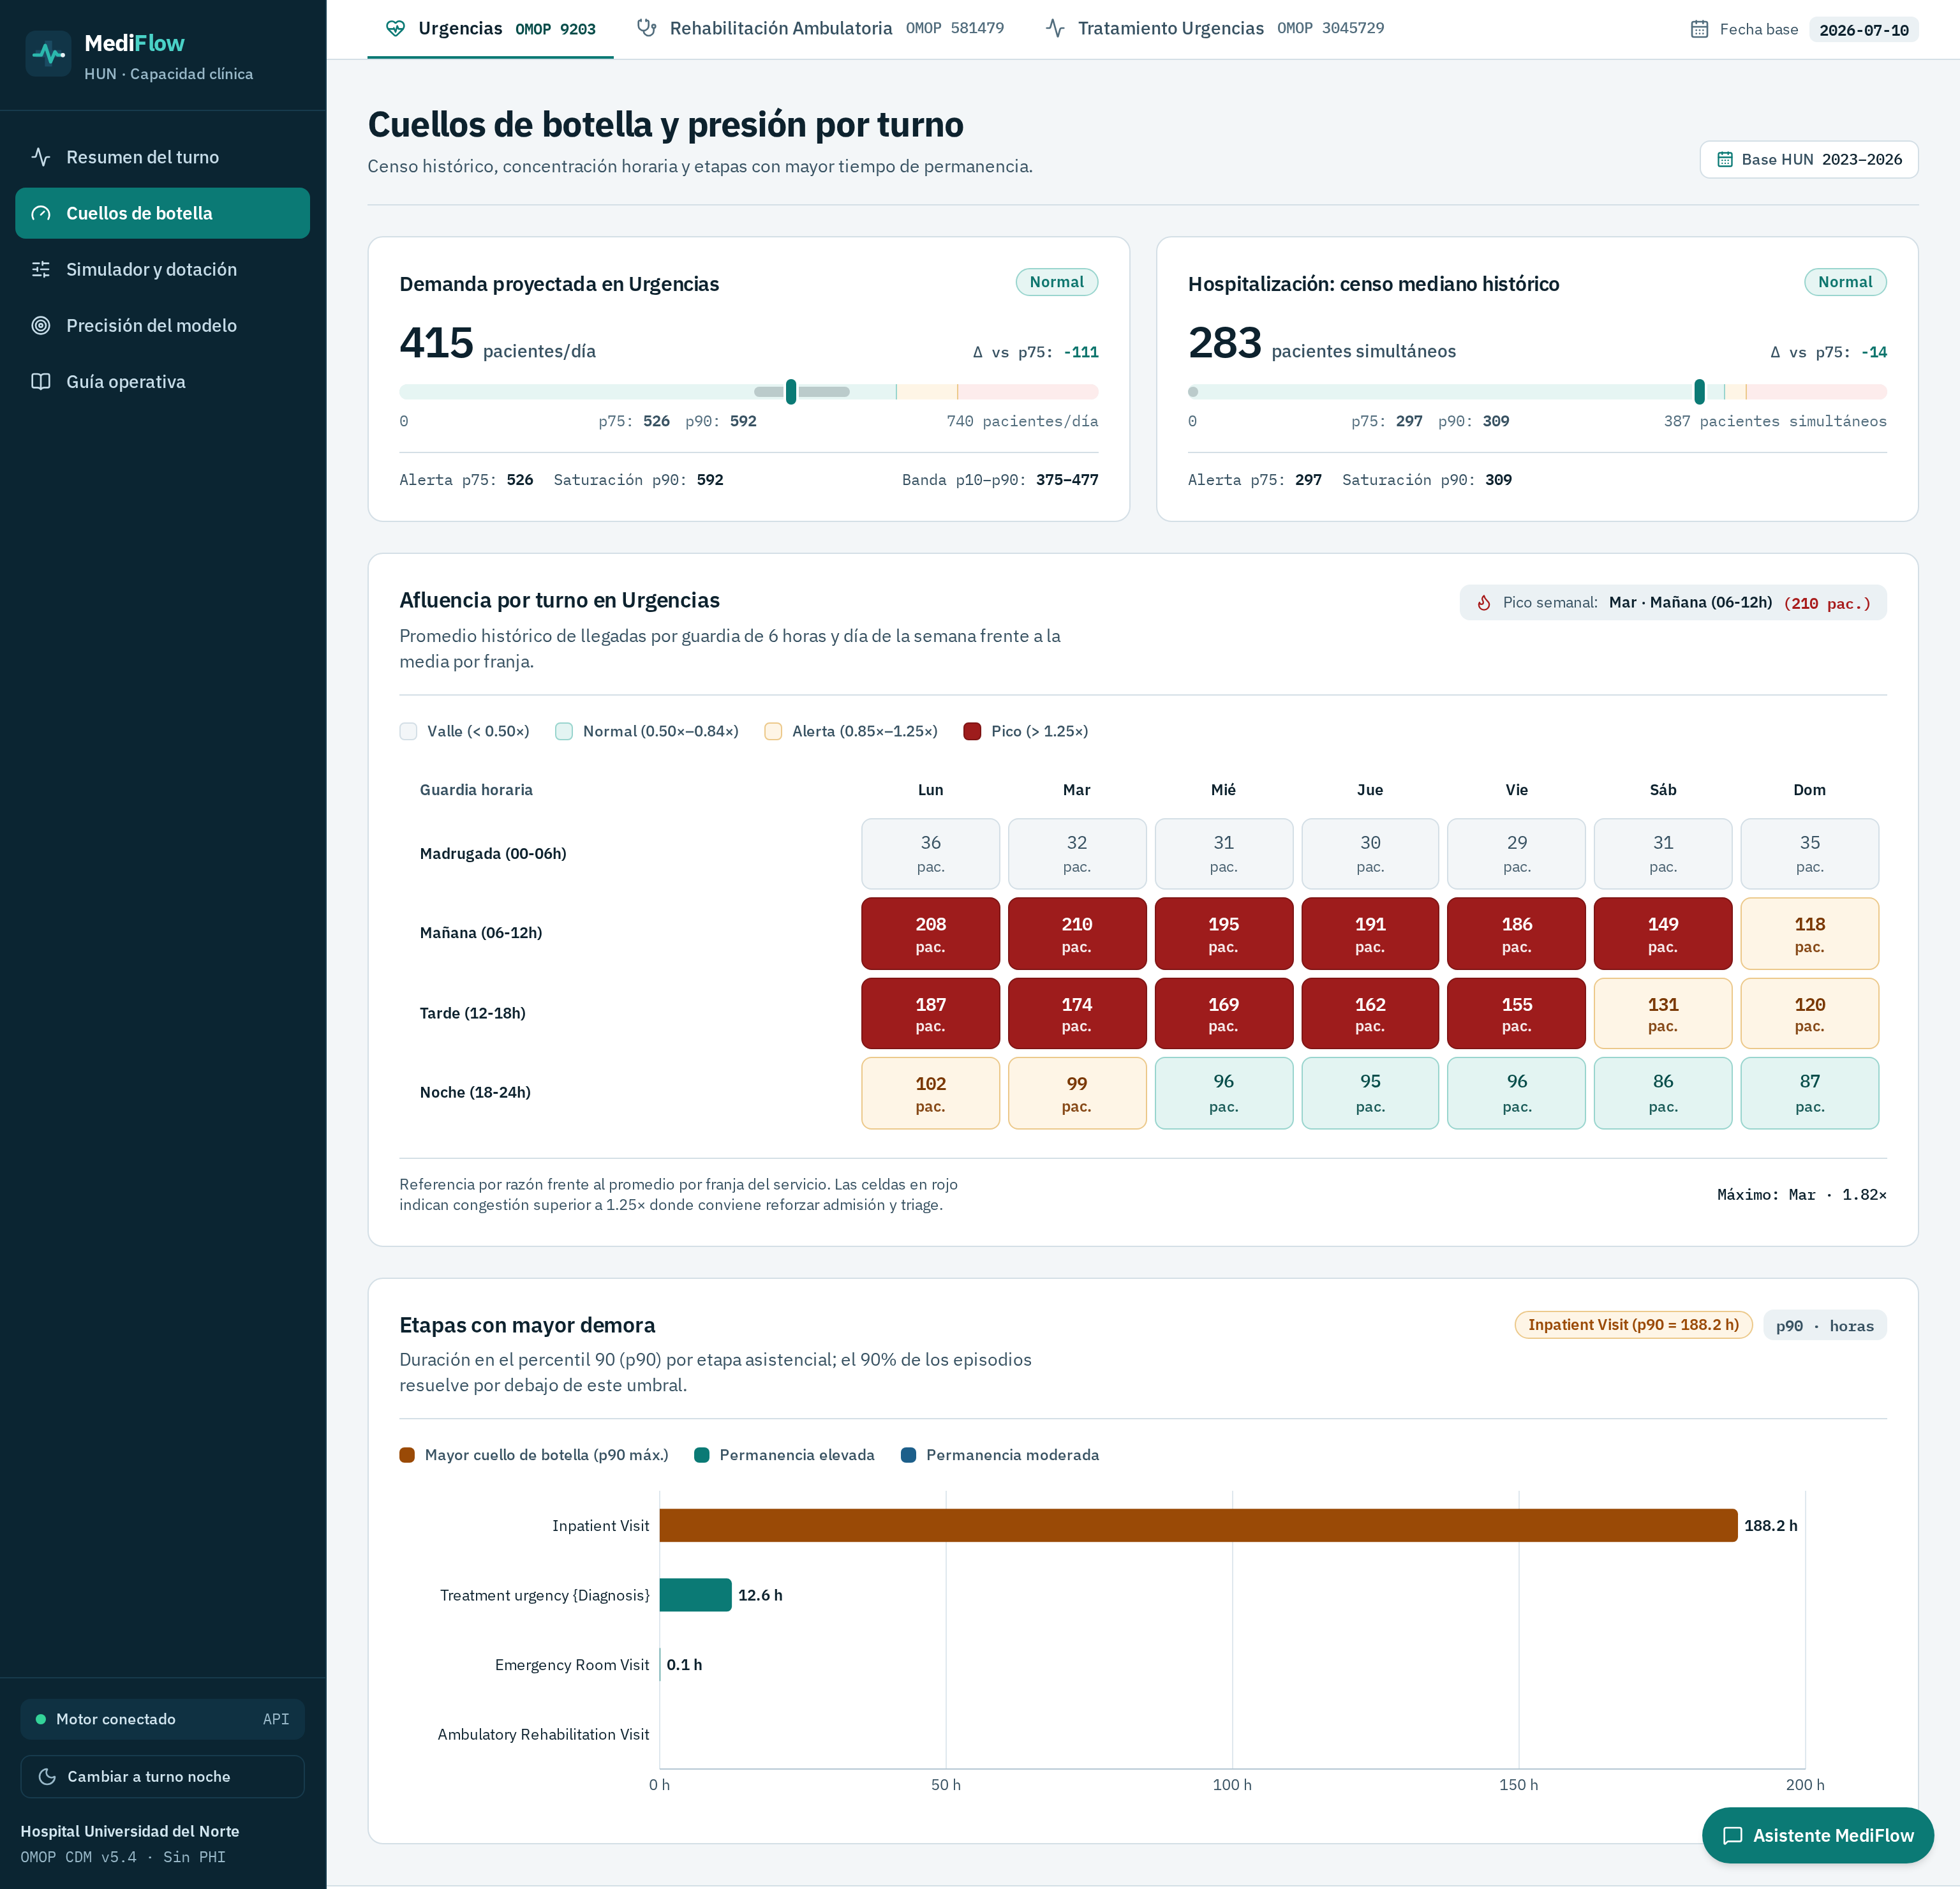
\includegraphics[width=0.92\textwidth]{cuellos_botella.png}
\apanota{Captura archivada del frontend (\texttt{docs/img/app/cuellos\_botella.png}). Muestra indicadores históricos de censo y duraciones por etapa provenientes de agregados del artefacto empaquetado; no representa una ejecución en vivo ni camas físicas habilitadas.}
\end{figure}

\begin{figure}[htbp]
\caption{Vista archivada de precisión histórica en Urgencias con el asistente abierto}
\label{fig:app_precision}
\centering
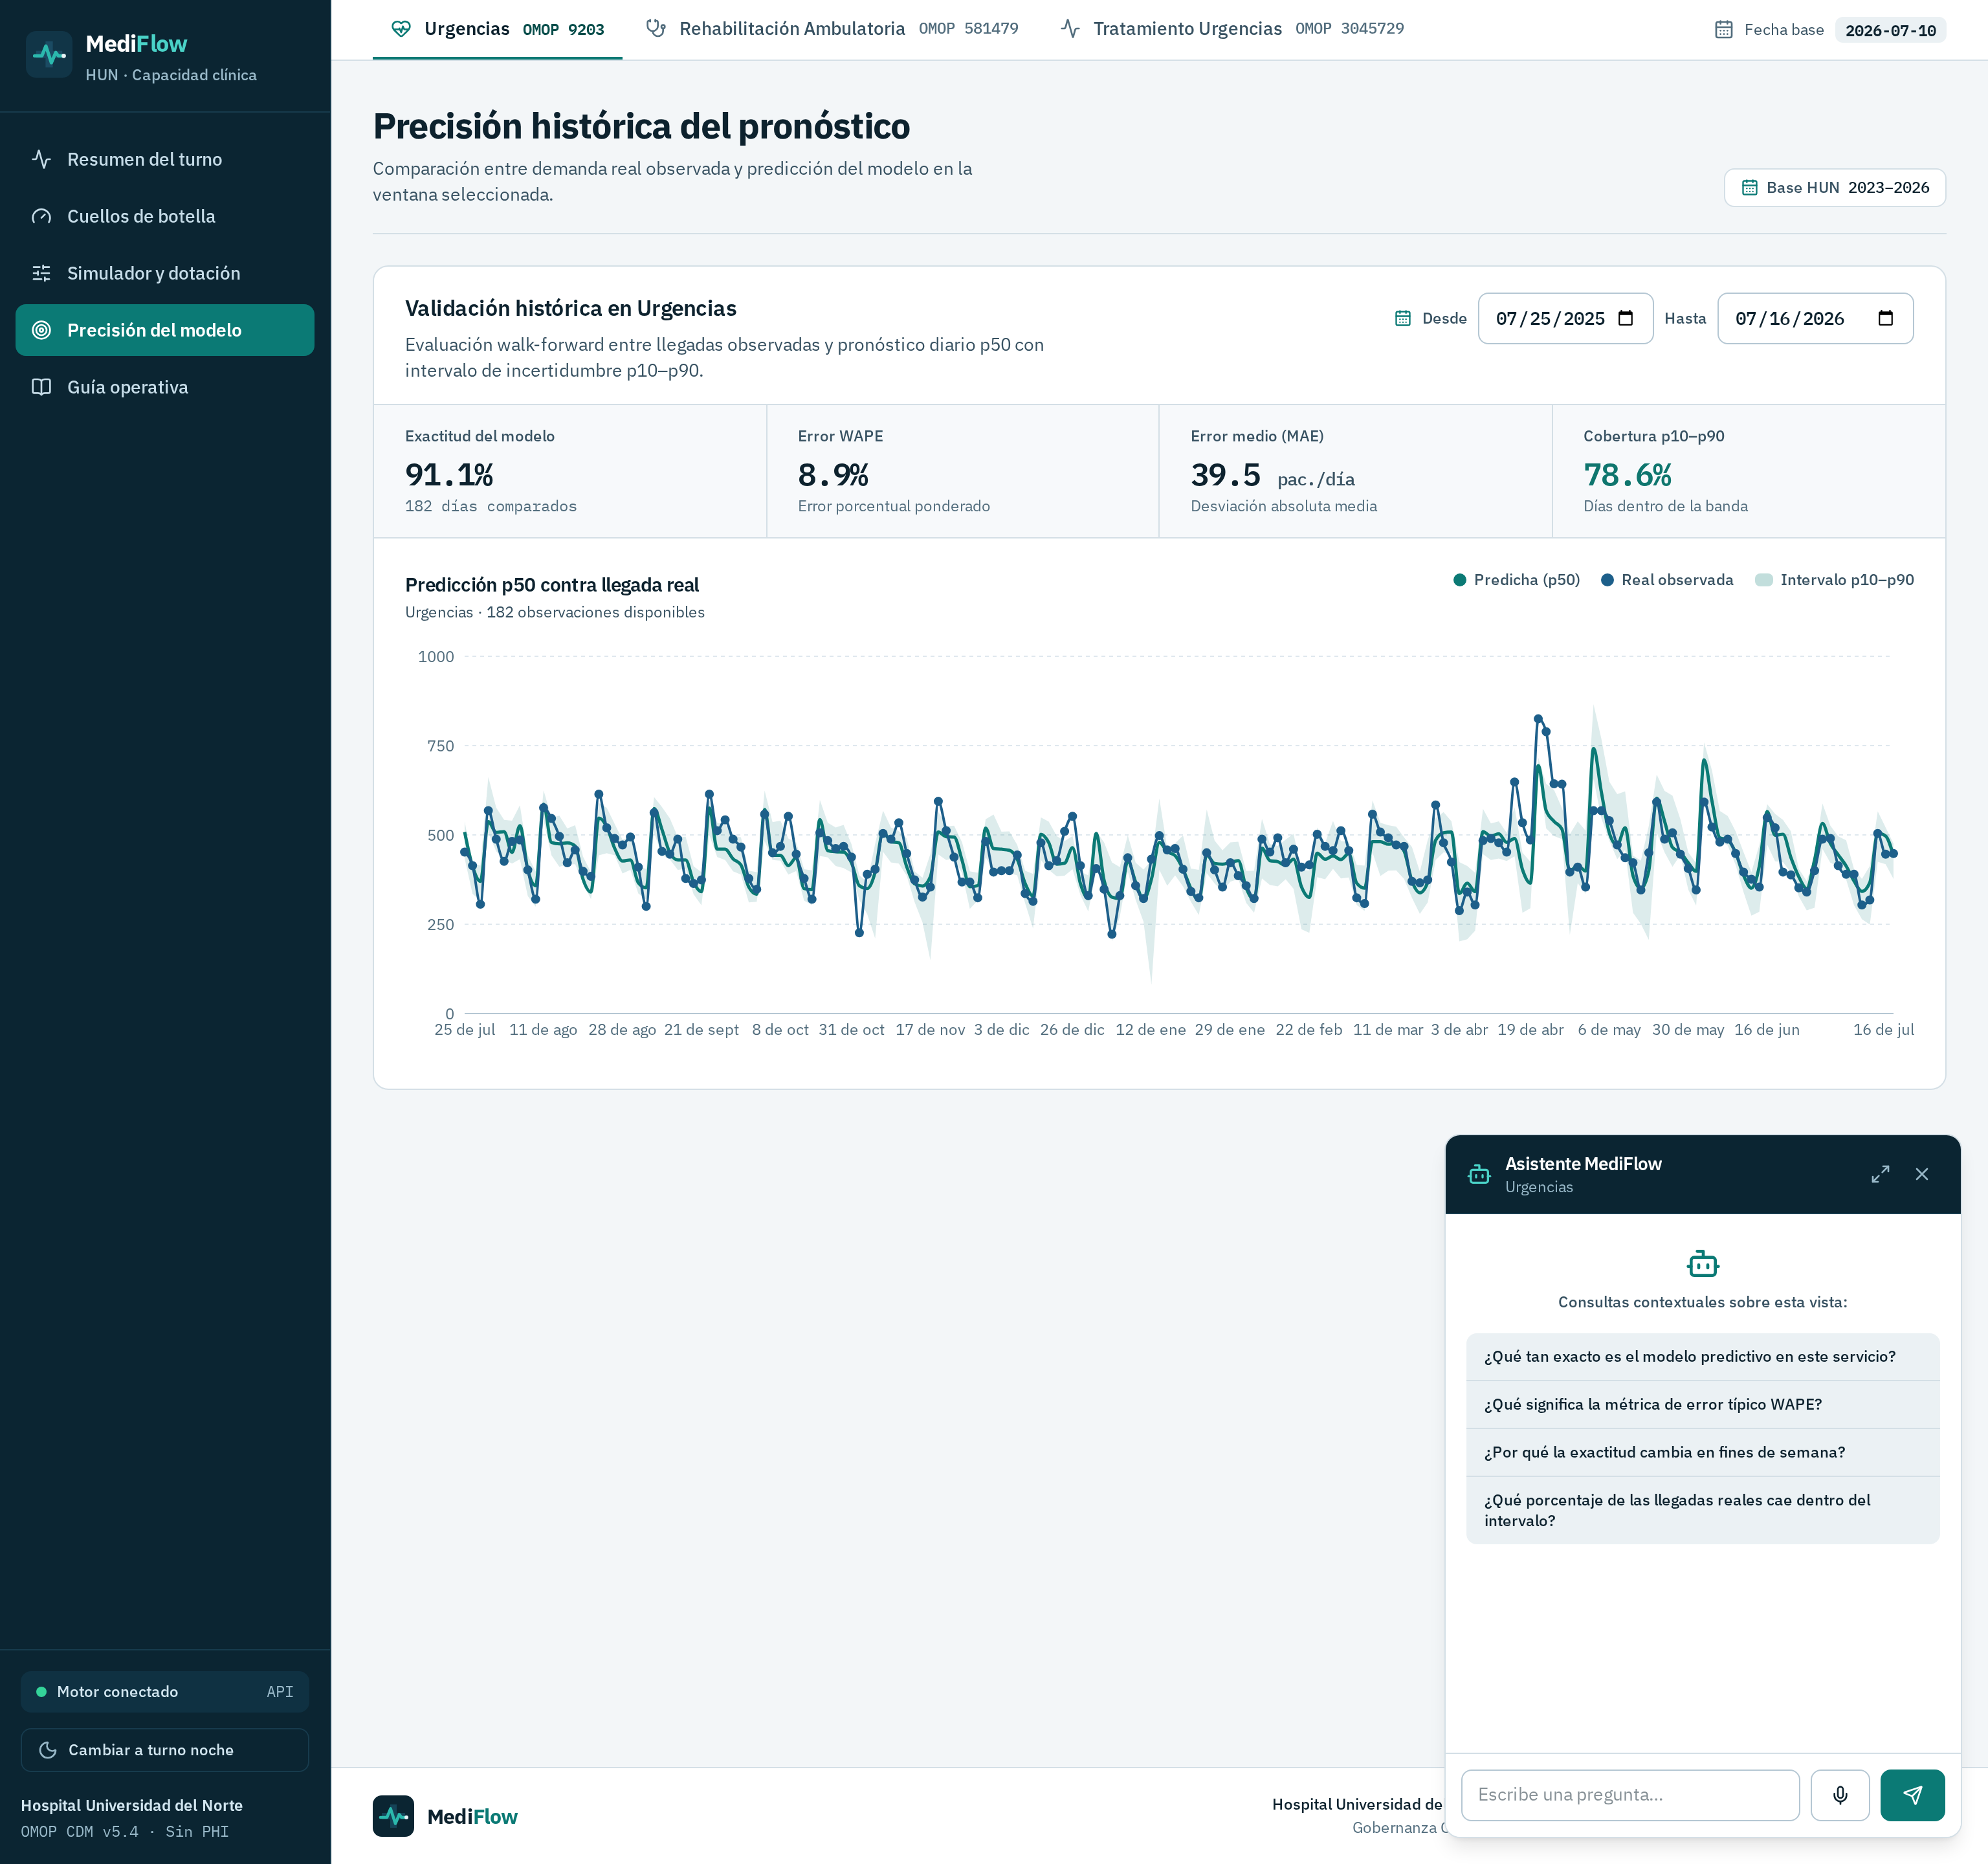
\includegraphics[width=0.92\textwidth]{precision_asistente.png}
\apanota{Captura archivada del frontend (\texttt{docs/img/app/precision\_asistente.png}). Los valores exhibidos (exactitud 91,1\,\%, WAPE 8,9\,\%, cobertura 78,6\,\% en 182 días) corresponden al modelo cuantílico del bundle \texttt{v2.0} y no al experimento puntual Poisson (WAPE 8,4\,\%).}
\end{figure}

\begin{figure}[htbp]
\caption{Captura compuesta archivada del simulador de optimización y escenarios}
\label{fig:app_simulador}
\centering
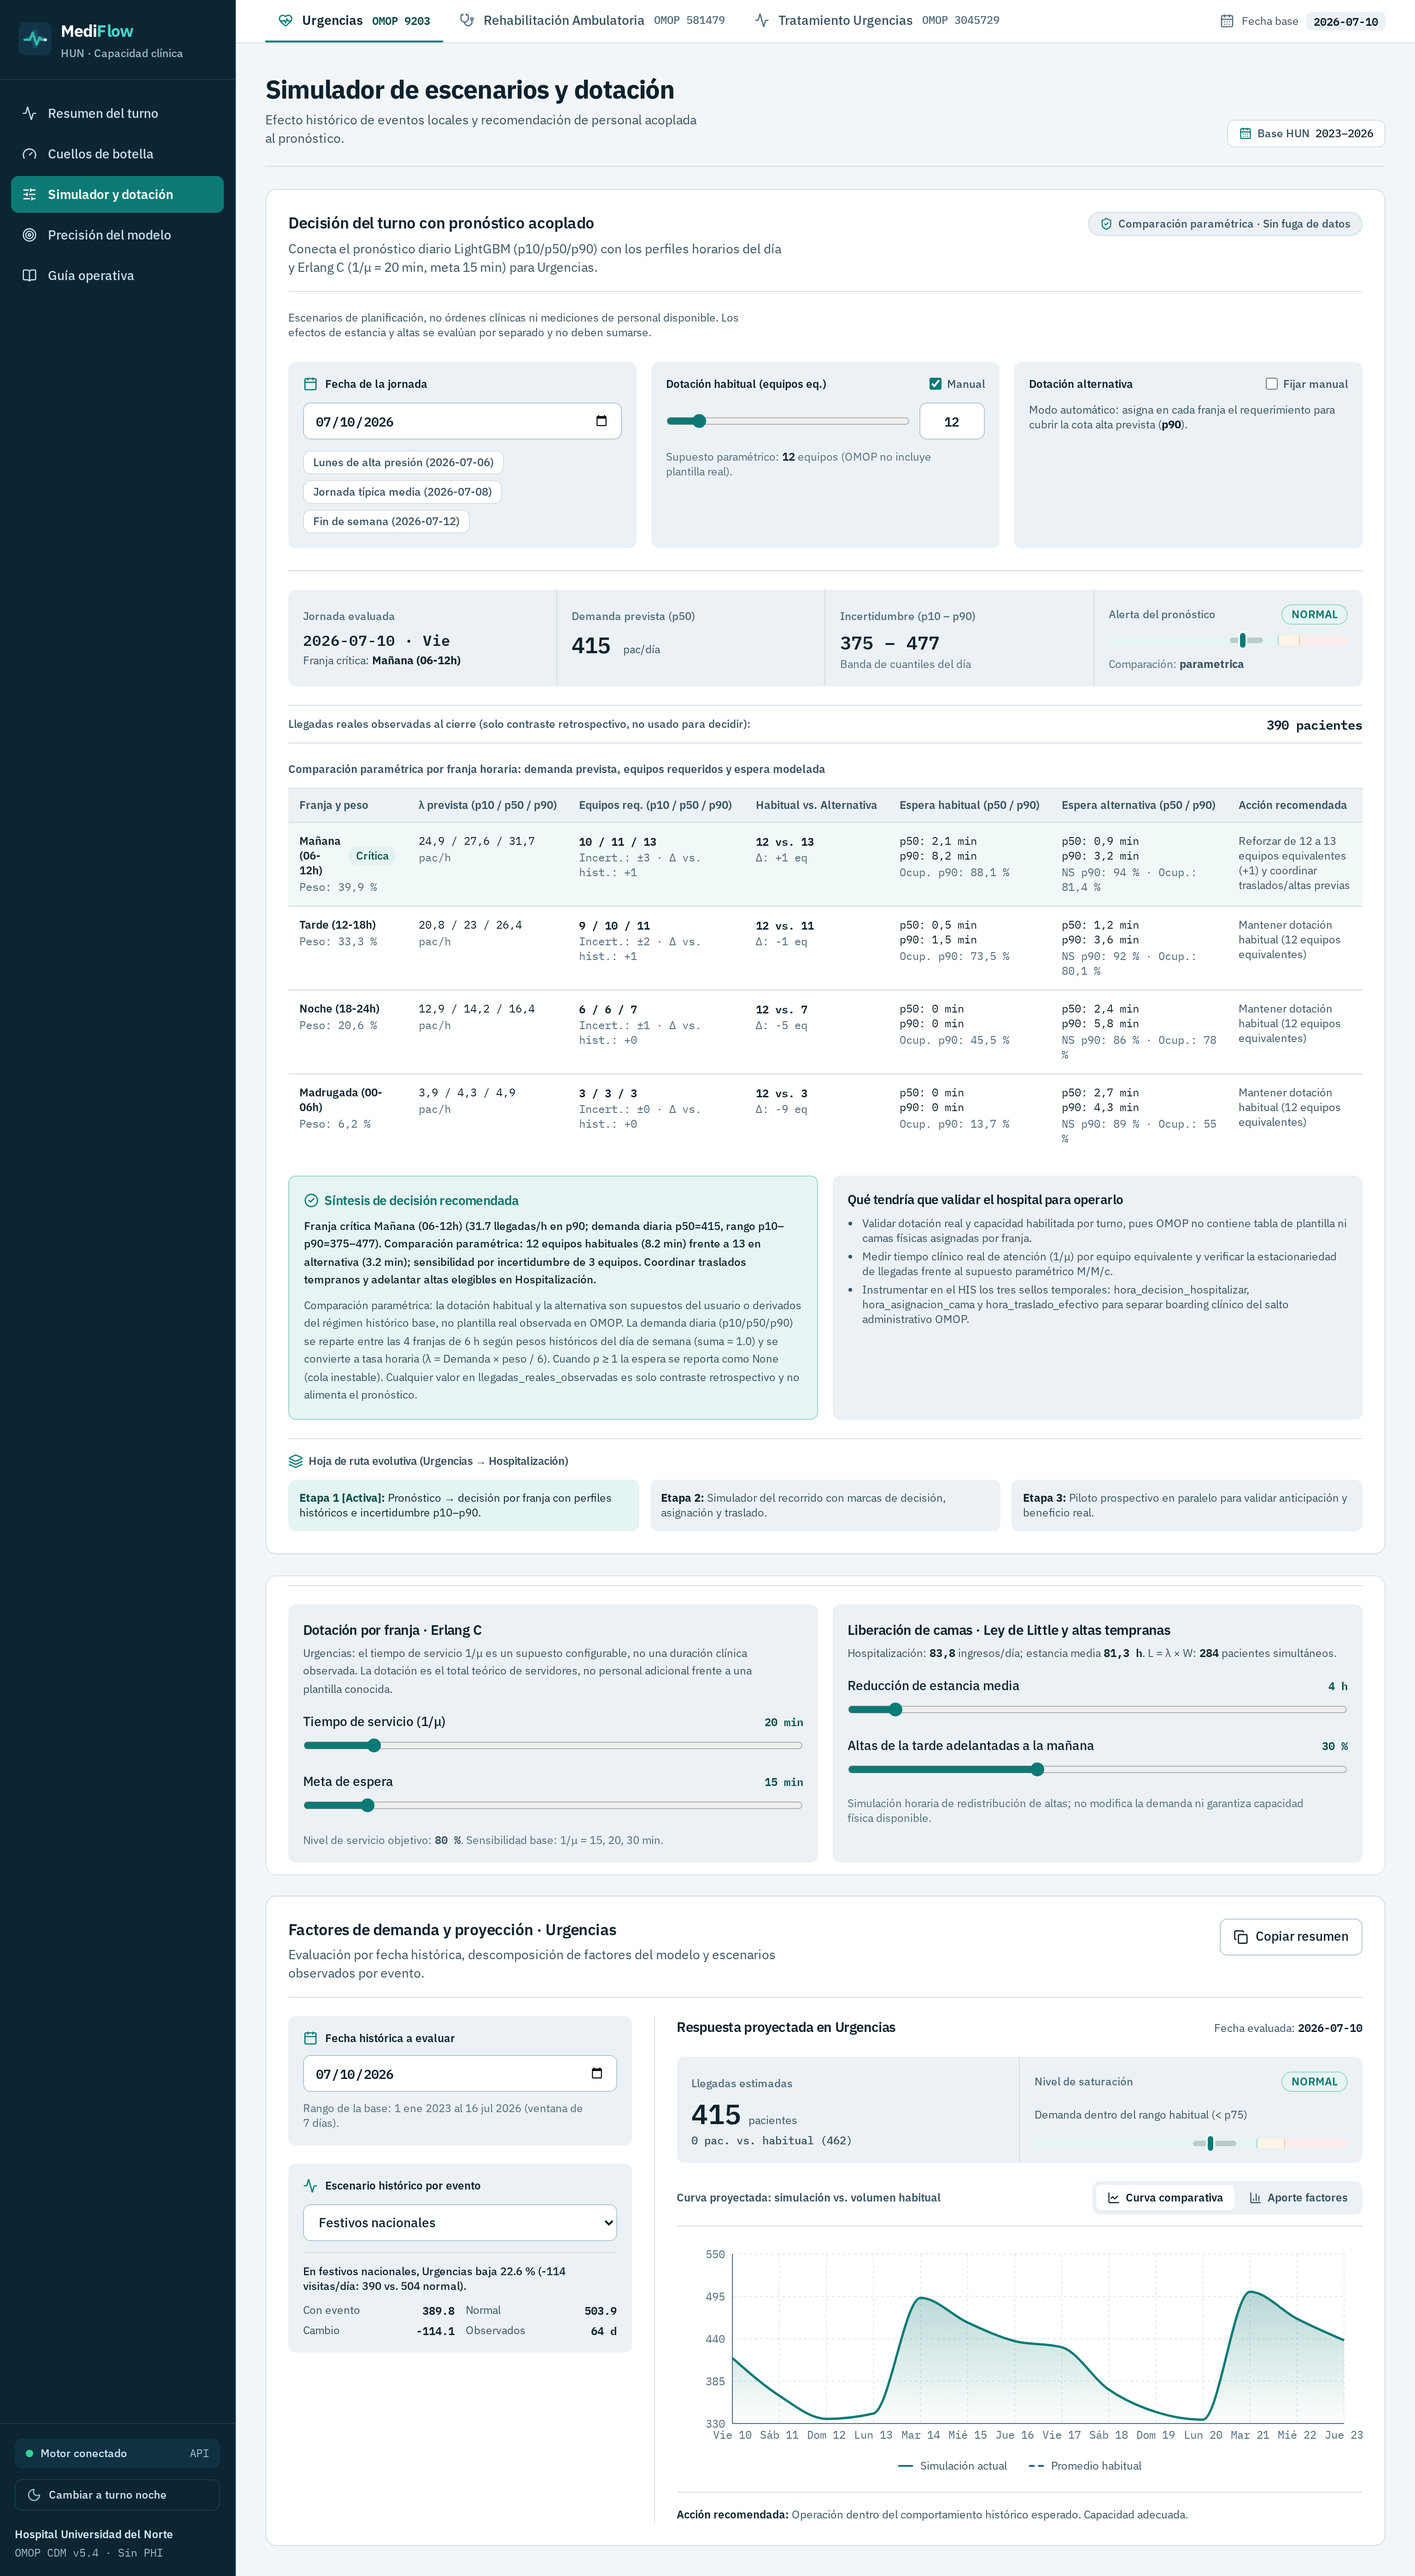
\includegraphics[width=0.92\textwidth,height=0.72\textheight,keepaspectratio]{simulador_optimizacion.png}
\apanota{Captura compuesta archivada (\texttt{docs/img/app/simulador\_optimizacion.png}) que reúne tres secciones verticales de la misma vista. Conserva rótulos anteriores («Etapa 1 [Activa]», «Sin fuga de datos» y referencia híbrida de 284 pacientes en Ley de Little); el código vigente del panel informa explícitamente la ausencia de perfiles por corte en el bundle \texttt{v2.0}.}
\end{figure}

\begin{figure}[htbp]
\caption{Vista archivada del tablero operativo de pronóstico de demanda}
\label{fig:app_dashboard}
\centering
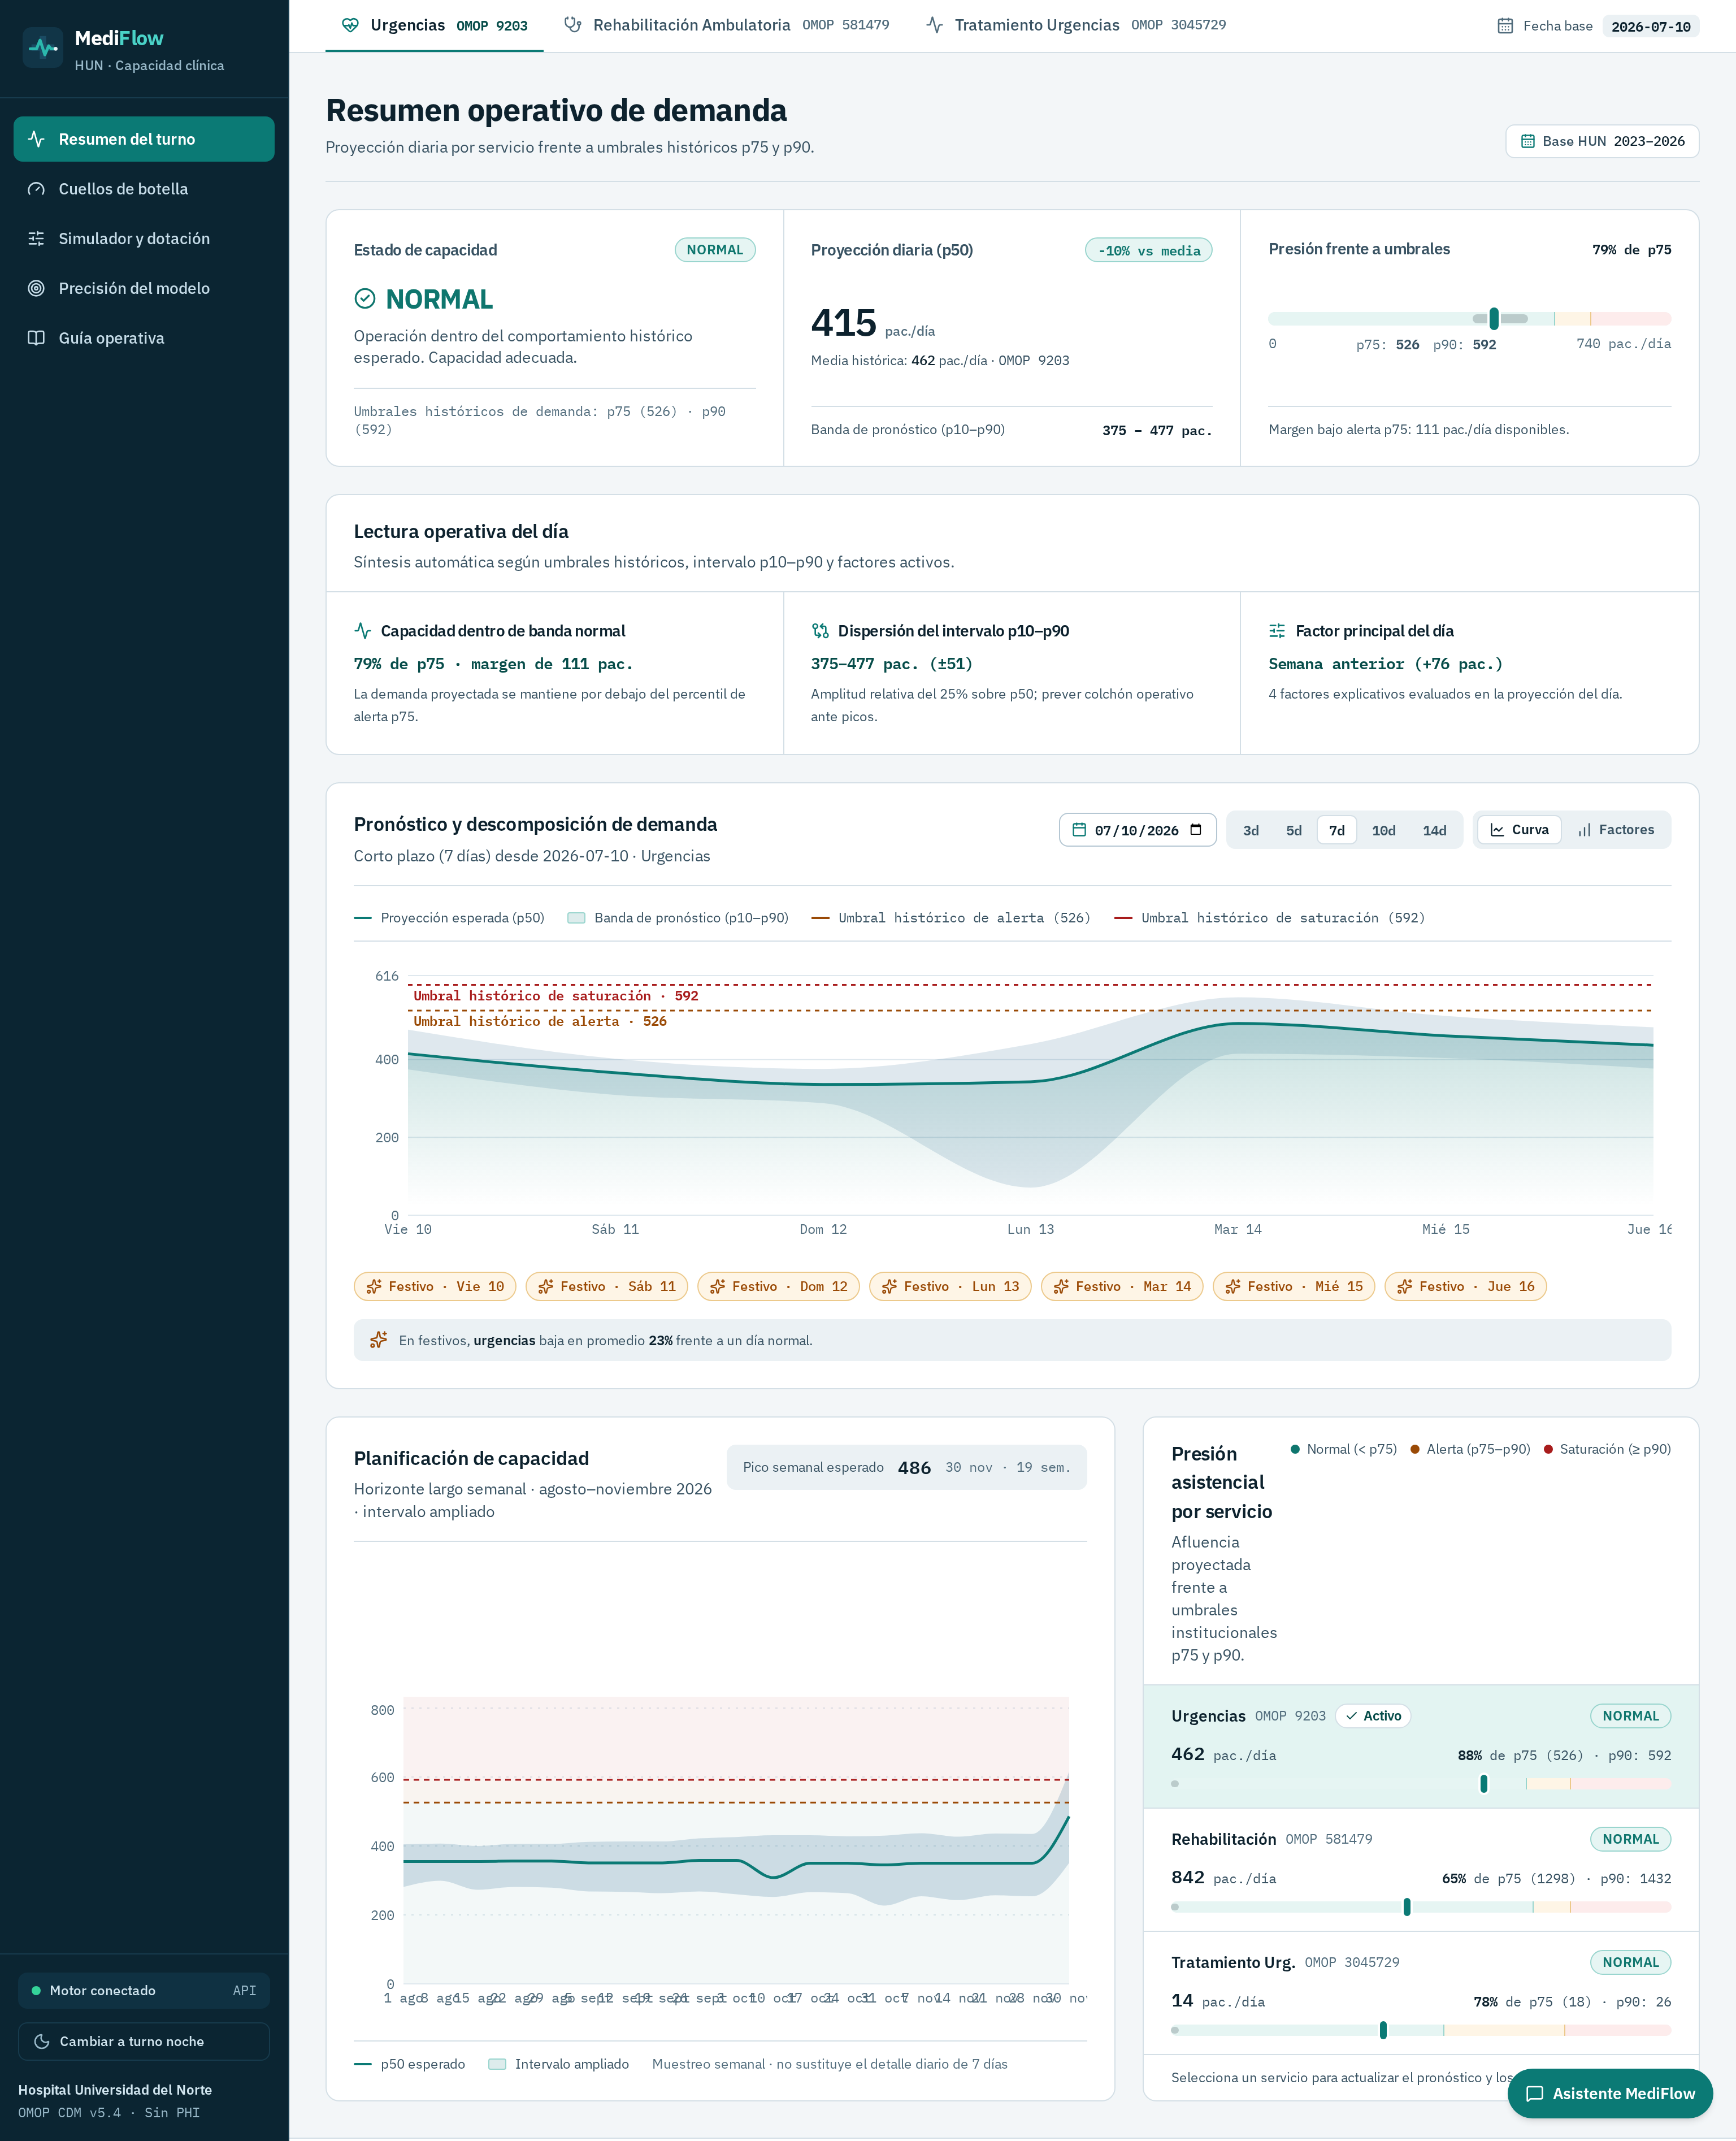
\includegraphics[width=0.92\textwidth,height=0.72\textheight,keepaspectratio]{dashboard_pronostico.png}
\apanota{Captura archivada del frontend (\texttt{docs/img/app/dashboard\_pronostico.png}). Advertencia de integridad visual: la imagen exhibe etiquetas de «Festivo» repetidas sobre los siete días del 10 al 16 de julio de 2026 y superposición de rótulos en el eje temporal del gráfico de largo plazo; debe interpretarse únicamente como ilustración general de diseño y nunca como fuente numérica de calendario ni de proyección.}
\end{figure}

% Sección 8: Ingeniería de software, reproducibilidad y privacidad
% evidencia:E24,E25,E29

\section{Ingeniería de software, reproducibilidad y privacidad}

La confiabilidad de MediFlow como plataforma analítica descansa sobre la separación modular del código fuente, la trazabilidad de dependencias, la cobertura de pruebas unitarias y de contrato, y la protección estricta de los registros hospitalarios frente a exposiciones accidentales \parencite{mediflow2026informe,mediflow2026auditoria}.

\subsection{Estructura real del código y dependencias}

La inspección directa del árbol de directorios del repositorio permite precisar la distribución efectiva de responsabilidades frente a descripciones genéricas de diseño previo:

\begin{itemize}[leftmargin=*,nosep]
\item \textit{Extracción y calidad} (\texttt{src/hun/data/}): agrupa la conexión de solo lectura (\texttt{conexion.py}), el ejecutor mensual resumible (\texttt{extraer.py}), las 24 consultas SQL (\texttt{sql/00\_*} a \texttt{sql/23\_*}), la regularización de series (\texttt{agregados.py}), las pruebas de consistencia temporal (\texttt{auditoria.py}), el mapeo de conceptos (\texttt{conceptos.py}) y la utilidad de borrado al cierre (\texttt{borrar\_datos.py}).
\item \textit{Modelado e inferencia} (\texttt{src/hun/models/}): concentra tanto la ingeniería de variables y rezagos como los modelos y reportes en los módulos \texttt{validacion.py}, \texttt{linea\_base.py}, \texttt{evaluacion\_}\allowbreak\texttt{factores.py}, \texttt{demanda.py}, \texttt{saturacion.py}, \texttt{explicacion.py}, \texttt{largo\_plazo.py}, \texttt{optimizacion.py}, \texttt{empaquetar.py} y \texttt{predict.py}. Por el contrario, los directorios \texttt{src/hun/features/}, \texttt{src/hun/visualization/} y \texttt{src/hun/external/} contienen únicamente archivos \texttt{\_\_init\_\_.py} con cadenas documentales (\textit{stubs}), sin lógica funcional implementada.
\item \textit{Pipeline de factores externos} (\texttt{src/external/}): reside fuera del paquete \texttt{hun} mediante los módulos \texttt{config.py}, \texttt{calendario.py}, \texttt{clima.py}, \texttt{epidemiologia.py} y \texttt{build.py}.
\item \textit{Capa web y análisis} (\texttt{app/} y \texttt{dashboards/}): la API FastAPI vive en \texttt{app/api/\_\_init\_\_.py} y \texttt{app/api/chat.py}; la interfaz React en \texttt{app/src/} (destacando \texttt{OptimizationPanel.jsx} y el contrato \texttt{optimizationPayload.test.js}); y la definición Power BI PBIP junto con \texttt{preparar\_modelo.py} en \texttt{dashboards/powerbi/}. Los cuadernos en \texttt{notebooks/} cumplen funciones exploratorias y se mantienen limpios de salidas mediante \texttt{nbstripout}.
\end{itemize}

Respecto de las dependencias declaradas, se observa una desalineación menor entre los manifiestos de Python: \texttt{pyproject.toml} (paquete \texttt{hun}, Python $\ge 3{,}11$) incluye el núcleo analítico (\texttt{pandas}, \texttt{numpy}, \texttt{scikit-learn}, \texttt{lightgbm}, \texttt{shap}, \texttt{pyarrow}, \texttt{holidays}, \texttt{python-dateutil}, \texttt{matplotlib}, \texttt{seaborn}, \texttt{plotly}, \texttt{requests}, \texttt{python-dotenv}) y extras opcionales (\texttt{sqlalchemy>=2.0}, \texttt{psycopg[binary]>=3.1}, \texttt{pytest}, \texttt{ruff}, \texttt{pre-commit}, \texttt{nbstripout}), pero omite \texttt{fastapi} y \texttt{uvicorn}; a su vez, \texttt{requirements.txt} sí declara \texttt{fastapi>=0.110.0} y \texttt{uvicorn>=0.28.0}, aunque conserva \texttt{streamlit} pese a haberse descartado en favor de React/Vite en \texttt{DEC-006}. En el frontend (\texttt{app/package.json}), las dependencias verificadas corresponden a React \texttt{19.3.1}, Recharts \texttt{3.10.1}, Lucide React \texttt{1.61.0}, Tailwind CSS \texttt{4.3.3} y Vite \texttt{8.3.4}.

\subsection{Evidencia de pruebas automatizadas frente a auditorías históricas}

Es fundamental separar las verificaciones locales del cierre de integración de las auditorías previas y de la validación clínica. La Tabla~\ref{tab:evidencia_pruebas} contrasta los distintos registros de verificación comprobados en el repositorio.

\begin{table}[htbp]
\caption{Niveles de verificación técnica y estado comprobado en el repositorio}
\label{tab:evidencia_pruebas}
{\singlespacing\small
\begin{tabularx}{\textwidth}{@{}L{0.22\textwidth} L{0.26\textwidth} L{0.23\textwidth} Y@{}}
\toprule
Evidencia & Alcance verificado & Estado en \texttt{803c1a1} & Qué no acredita \\
\midrule
Recolección estática local (\texttt{pytest}, Node) & 180 pruebas Python en 13 archivos \texttt{test\_*.py} + 3 pruebas Node & Comprobado por recolección (\texttt{--collect-only}) & No equivale a nueva corrida de modelos ni reejecución de suite \\
Cierre de integración (\nolinkurl{cierre_auditoria.md}) & 180/180 Python (211,30\,s; corrida de 228,50\,s en \nolinkurl{tests/README.md}), 3/3 Node, build Vite, Ruff, API con Parquet bloqueado & Ejecución previa documentada al integrar \texttt{main} & No prueba calibración sobre BD, eficacia clínica ni despliegue público \\
Validación independiente (\texttt{2026-11-03}) & Revisión interna Sprint 2/3 sobre arquitectura anti-fuga con 103/103 pruebas & Registro histórico superado por el cierre de 180 pruebas & No es revisión ciega externa ni autorización médica \\
\bottomrule
\end{tabularx}}
\apanota{Fuentes contrastadas: \textcite{mediflow2026auditoria}, \textcite{mediflow2026validacion} y \texttt{tests/README.md}. Para este informe LaTeX no se reejecutó la suite completa de 180 pruebas ni se regeneró el artefacto \texttt{joblib}; únicamente se verificó el conteo estático de pruebas recopiladas.}
\end{table}

\subsection{Tres niveles de reproducibilidad y controles de privacidad}

MediFlow distingue tres niveles crecientes de reproducción según los insumos disponibles en el entorno \parencite{mediflow2026informe,mediflow2026auditoria}:

\begin{enumerate}[leftmargin=*,nosep]
\item \textit{Nivel 1 (fixtures sintéticos y contratos de software)}: accesible en cualquier clon limpio de GitHub sin credenciales ni datos hospitalarios mediante \texttt{pytest -q}, \texttt{node --test app/src/lib/optimizationPayload.test.js} y \texttt{npm --prefix app run build}. Incluye la verificación de la ruta completa Etapa~1 (\texttt{v2.1}) con datos sintéticos explícitos.
\item \textit{Nivel 2 (inferencia estricta con artefacto autorizado)}: permite levantar el servidor FastAPI y la interfaz web consumiendo únicamente \texttt{models/modelos\_web\_bundle.joblib} con \texttt{HUN\_MODO\_PRODUCCION=1}, sin carpeta \texttt{data/}. Su distribución exige autorización explícita por contener salidas y pesos agregados del hospital.
\item \textit{Nivel 3 (reproducción hospitalaria completa)}: requiere conectividad VPN FortiClient, credenciales de solo lectura en \texttt{.env} y los archivos agregados privados (\texttt{data/raw/*.parquet}, \texttt{data/externos.parquet}) excluidos del control de versiones para reextraer SQL y reentrenar todos los módulos. No ha sido reejecutado en esta consolidación editorial.
\end{enumerate}

En materia de privacidad y gobernanza de datos, \texttt{src/hun/data/conexion.py} impone en PostgreSQL el parámetro de sesión \texttt{default\_transaction\_read\_only=on}, límites de tiempo (\texttt{statement\_timeout=120\,s}) y validación sintáctica en Python que rechaza cualquier sentencia distinta de \texttt{SELECT} o \texttt{WITH} y bloquea palabras clave de escritura o alteración. El archivo \texttt{.gitignore} excluye \texttt{data/raw/}, \texttt{data/processed/}, archivos \texttt{.parquet}, credenciales \texttt{.env} y archivos \texttt{.pbix} o cachés locales de Power BI, mientras \texttt{borrar\_datos.py} y \texttt{docs/cierre\_datos.md} formalizan el protocolo de eliminación de datos al concluir el reto \parencite{mediflow2026auditoria}. No obstante, estos controles técnicos no sustituyen la revisión jurídica ni el análisis de riesgo de reidentificación por celdas pequeñas antes de publicar tableros o servicios web en entornos externos o en la nube.

% Sección 9: Discusión, recomendaciones accionables y limitaciones
% evidencia:E16,E17,E18,E19,E20,E23,E27

\section{Discusión, recomendaciones accionables y limitaciones}

El valor práctico de MediFlow no radica en ofrecer cifras únicas de exactitud ni en automatizar decisiones clínicas, sino en articular datos administrativos heterogéneos bajo criterios cuantitativos auditables, dejando explícitos sus supuestos y márgenes de error. Una interpretación responsable exige contrastar los hallazgos numéricos frente a hipótesis alternativas y frente al estado real de implementación de cada componente.

\subsection{Interpretación operativa e hipótesis alternativas}

Los resultados predictivos confirman una frontera clara entre servicios de alto volumen y servicios de conteo bajo o intermitente. En Urgencias (8,4\,\% WAPE en \texttt{lgbm\_final}; 8,91\,\% en bundle \texttt{v2.0}) y Rehabilitación Ambulatoria entre lunes y viernes (85,6\,\%--90,9\,\% de exactitud), la combinación de rezagos semanales y calendario colombiano permite anticipar oscilaciones semanales y cierres festivos con error acotado. En contraste, en Tratamiento Urgencias ($\approx 15{,}2$ llegadas/día, WAPE 43,5\,\% en \texttt{lgbm\_final} y 42,18\,\% en \texttt{v2.0}) y en los fines de semana de Rehabilitación (exactitud de 51,3\,\% los sábados y 15,6\,\% los domingos), la métrica porcentual refleja tanto la sensibilidad de denominador pequeño como desplazamientos semanales de tasa por debajo del techo Poisson idealizado (77,0\,\% semanal observado frente a 92,3\,\% teórico en el experimento puntual) \parencite{mediflow2026demanda}. En consecuencia, la planificación en Tratamiento Urgencias debe apoyarse en el error absoluto medio (MAE $\approx 6{,}4$--$6{,}6$ pacientes/día) y en agregados semanales, evitando prometer alertas diarias precisas en porcentaje.

En el componente de congestión hospitalaria, la verificación archivada de Ley de Little ($277{,}52$ frente a $277{,}47$ pacientes medios en población alineada) confirma la consistencia matemática del censo reconstruido tras el recorte $p_{99{,}9}$ \parencite{mediflow2026informe}. Al mismo tiempo, dos resultados previenen interpretaciones simplistas. Primero, la correlación ecológica negativa ($r = -0{,}481$) entre el censo mensual de Hospitalización y la espera $p_{90}$ en la transición Tratamiento Urgencias $\rightarrow$ Hospitalización ($25{,}13$\,h en meses normales frente a $23{,}70$\,h en meses de censo alto) muestra que las demoras registradas entre marcas OMOP no responden linealmente a la saturación mensual agregada de piso; pueden obedecer a prácticas de cierre administrativo tardío, flujos por tipo de ingreso o solapamientos entre registros \parencite{mediflow2026optimizacion}. Segundo, la simulación de altas tempranas demuestra que desplazar el 35\,\% de egresos de la tarde a la mañana reduce las horas en estado crítico de 9,32\,\% a 6,26\,\% ($-32{,}8\,\%$ relativo; $-3{,}06$\,pp), pero deja intacto el máximo histórico de 359 pacientes. La descongestión modelada actúa sobre la duración acumulada de la presión, no sobre los picos extremos.

\subsection{Estado consolidado de capacidades implementadas y pendientes}

Para impedir que se confunda código versionado o ensayos sintéticos con capacidades desplegadas sobre datos hospitalarios reales, la Tabla~\ref{tab:estado_capacidades} sintetiza la situación exacta de cada componente al corte del commit \texttt{803c1a1}.

\begin{table}[htbp]
\caption{Estado verificado de capacidades entre código, artefacto servido y pendientes}
\label{tab:estado_capacidades}
{\singlespacing\small
\begin{tabularx}{\textwidth}{@{}L{0.22\textwidth} L{0.25\textwidth} L{0.24\textwidth} Y@{}}
\toprule
Capacidad o módulo & Implementación en código & Estado en bundle \texttt{v2.0} / PBIP & Trabajo pendiente \\
\midrule
Pronóstico puntual 1--7\,d (\texttt{lgbm\_final} Poisson) & Implementado en \texttt{demanda.py} con nivel local y recencia & No es el modelo servido; reporte archivado del \texttt{2026-11-18} & Evaluar incorporación de nivel local en familia cuantílica \\
Pronóstico cuantílico web ($p_{10}/p_{50}/p_{90}$ + SHAP) & Implementado en \texttt{explicacion.py} y \texttt{predict.py} & Activo en bundle \texttt{v2.0} (corte \texttt{2026-07-17}) & Recalibrar cobertura (64,3\,\%--78,6\,\%) e incluir Carnaval/Semana Santa \\
Largo plazo a 120 días & Implementado en \texttt{largo\_plazo.py} (banda base $p_{05}/p_{95}$ ensanchada) & Activo vía \texttt{/api/largo-plazo} (corrida propia en \texttt{v2.0}) & Reconciliar reporte del \texttt{2026-11-03} frente a corrida empaquetada \\
Erlang~C histórico, Little y altas tempranas & Implementado en \texttt{optimizacion.py} (interpolación en API) & Activo en \texttt{v2.0} con Little híbrido (\num{284,01} pac.) & Regenerar artefacto con Little alineado (\num{277,52}) y medir $1/\mu$ real \\
Acoplamiento por corte Etapa~1 (\texttt{perfiles\_horarios}) & Implementado en \texttt{empaquetar.py} (\texttt{v2.1}) y probado con fixtures & No habilitado en \texttt{v2.0}: devuelve \texttt{disponible: false} & Regenerar paquete \texttt{v2.1} autorizado con perfiles sin fuga \\
Asistente \texttt{/api/chat} & 6 herramientas deterministas + respaldo offline (\texttt{chat.py}) & Operativo contra salidas del bundle vía FastAPI & Validar funcionamiento end-to-end con clave autorizada en despliegue \\
Tablero Power BI (PBIP) & 7 pág., 12 tab., 18 rel., 43 medidas DAX (\texttt{FechaCorte = 2026-04-30}) & Solo definiciones locales corregidas; sin datos en PBIP & Revisar en Desktop, alinear corte abril vs. julio y republicar enlace \\
Simulador de recorrido (Etapa~2) y piloto en sombra (Etapa~3) & Diseño conceptual documentado en \texttt{informe\_final.md} & No implementado en software ni validado en clínica & Instrumentar 3 marcas HIS, capacidad real y aprobar piloto \\
\bottomrule
\end{tabularx}}
\apanota{Consolidación basada en \textcite{mediflow2026auditoria}, \textcite{mediflow2026bundle}, \textcite{mediflow2026pbip} y la inspección directa de \texttt{src/hun/models/} y \texttt{app/}.}
\end{table}

\subsection{Recomendaciones condicionadas y hoja de ruta evolutiva}

Las cinco recomendaciones formuladas en la Tabla~\ref{tab:recomendaciones} (\texttt{REC-01} a \texttt{REC-05}) sintetizan los escenarios cuantificados del sistema \parencite{mediflow2026optimizacion,mediflow2026informe}. Todas tienen carácter de propuestas condicionadas a validación institucional previa; no constituyen compromisos acordados con las jefaturas del HUN ni proyecciones de ahorro económico o dotación contractual.

\begin{table}[htbp]
\caption{Recomendaciones operacionales condicionadas (\texttt{REC-01} a \texttt{REC-05}) y criterios de validación}
\label{tab:recomendaciones}
{\singlespacing\small
\begin{tabularx}{\textwidth}{@{}l L{0.24\textwidth} L{0.30\textwidth} Y@{}}
\toprule
ID & Acción propuesta & \shortstack[l]{Resultado modelado\\o archivado} & Condición e indicador de piloto \\
\midrule
\texttt{REC-01} & Validar equipos equivalentes en Urgencias (06--12\,h) & A demanda $p_{90}$ (39,67/h): 15 equipos frente a 12 normales; espera media 6,09\,min & Medir duración clínica real frente al supuesto de 20\,min y plantilla instalada por turno \\
\texttt{REC-02} & Revisar capacidad de Rehabilitación (06--12\,h) & A demanda $p_{90}$ (133,33/h): 70 equipos frente a 42 normales; espera media 5,30\,min & Contrastar agenda programada, atención supuesta (30\,min) y puestos simultáneos \\
\texttt{REC-03} & Investigar demoras evitables en estancia de Hospitalización & Reducir 4\,h libera teóricamente 13,97 camas medias equivalentes (4,92\,\% del Little híbrido) & Auditar causas administrativas de egreso manteniendo intactos los criterios clínicos de alta \\
\texttt{REC-04} & Pilotar egreso seguro intradía en altas elegibles & Adelantar 35\,\% de [14,20) a [08,12): horas rojas 9,32\,\% $\rightarrow$ 6,26\,\% ($-32{,}8\,\%$ rel.); pico 359 & Evaluar en piloto con umbral fijo ($>309$), tasa de reingreso y seguridad del alta \\
\texttt{REC-05} & Auditar sellos temporales en Tratamiento Urg. $\rightarrow$ Hosp. & \num{47670} pasos; $p_{90}$ mensual ponderado 24,45\,h; correlación con censo $r = -0{,}481$ & Instrumentar decisión, asignación de cama y traslado efectivo antes de atribuir demora a cama \\
\bottomrule
\end{tabularx}}
\apanota{Propuestas extraídas de \textcite{mediflow2026optimizacion} y \textcite{mediflow2026informe}. Los porcentajes y camas medias equivalentes representan escenarios retrospectivos o paramétricos; los indicadores sugeridos para una eventual fase piloto (demora efectiva de traslado, estancia observada, horas en alerta roja a umbral fijo y métricas de seguridad clínica) no implican metas institucionales aprobadas ni calendario confirmado.}
\end{table}

La hoja de ruta para trasladar estas propuestas a operación asistencial se estructura en tres etapas secuenciales \parencite{mediflow2026informe}: (1) completar el paquete \texttt{v2.1} sobre agregados autorizados incorporando perfiles horarios por corte, reconciliando el valor de Little con población común y recalibrando cuantiles por servicio; (2) desarrollar el simulador de recorrido integrando camas habilitadas, dotación efectiva, tiempos de atención medidos y tres sellos del HIS (\texttt{hora\_decision\_hospitalizar}, \texttt{hora\_asignacion\_cama} y \texttt{hora\_traslado\_efectivo}); y (3) ejecutar un piloto prospectivo en modo sombra paralelo a la operación habitual antes de validar cualquier intervención asistencial supervisada.

\subsection{Limitaciones consolidadas}

Seis limitaciones estructurales acotan el uso actual de MediFlow: (a) ausencia en OMOP de camas físicas habilitadas, dotación de personal y tiempos clínicos de atención, obligando a trabajar con equipos equivalentes y umbrales históricos relativos; (b) carácter estadístico del recorte $p_{99{,}9}$ sobre estancias extremas y exclusión de variables clínicas de diagnóstico, procedimiento o laboratorio en la matriz predictiva; (c) ambigüedad administrativa de \texttt{espera\_h} en transiciones con posibles solapamientos negativos; (d) cobertura desigual en los intervalos cuantílicos del bundle \texttt{v2.0} (inferiores a 80\,\% nominal en los tres servicios sobre 182 días) y ausencia de perfiles por corte en el binario actual; (e) divergencia temporal entre Power BI (corte abril 2026 sin verificación de republicación) y demanda (corte julio 2026), así como entre los dos reportes comprobados de largo plazo; y (f) inexistencia de validación prospectiva en vivo o autorización clínica para decisiones asistenciales directas.

% Sección 10: Conclusiones y trabajo futuro

\section{Conclusiones y trabajo futuro}

MediFlow entrega una base analítica reproducible e interpretable para estudiar la demanda y la presión operativa del Hospital Universidad del Norte a partir de agregados compatibles con OMOP CDM v5.4, articulando comprensión del flujo histórico, predicción con evaluación temporal estricta y exploración paramétrica de escenarios bajo supuestos declarados. La verificación empírica en el corte documental del repositorio (\texttt{803c1a1}) confirma un contraste riguroso entre fuentes: en el experimento puntual LightGBM Poisson con nivel local (\texttt{lgbm\_final}), el WAPE diario global desciende de 18,0\,\% a 10,5\,\% (mejora relativa archivada de 41,6\,\%) con sólido desempeño en Urgencias (8,4\,\%) y Rehabilitación laboral, mientras que el artefacto cuantílico efectivamente servido en la web (\texttt{v2.0}) exhibe WAPE de 8,91\,\%, 11,08\,\% y 42,18\,\% por servicio con coberturas de 78,57\,\%, 64,29\,\% y 73,08\,\% sobre 182 días. En Hospitalización, la verificación documentada de stock inicial nulo en 12 cortes y de Ley de Little sobre población común depurada por $p_{99{,}9}$ (\num{277,52} pacientes frente a \num{277,47} de media horaria) aporta consistencia interna sólida, al tiempo que la simulación de adelanto del 35\,\% de altas vespertinas estima una reducción relativa de 32,8\,\% en horas rojas (9,32\,\% a 6,26\,\%) sin reducir el pico máximo de 359 pacientes.

Estos resultados retrospectivos justifican avanzar hacia una validación operativa supervisada, pero no demuestran beneficio clínico ni sustituyen las mediciones físicas del hospital. Quedan priorizadas cinco líneas de trabajo inmediato antes de un despliegue institucional: (1) regenerar el artefacto web hacia la versión \texttt{v2.1} desde agregados autorizados para habilitar \texttt{perfiles\_horarios} reales por corte y unificar Ley de Little sobre la población alineada; (2) recalibrar los intervalos cuantílicos e incorporar la selección completa de factores externos aceptados y nivel local dentro del paquete servido, reconciliando además las métricas de largo plazo entre el reporte histórico y el artefacto; (3) abrir, revisar visualmente y republicar el proyecto PBIP de Power BI aclarando o unificando la brecha de corte entre abril y julio de 2026; (4) auditar los sellos temporales de transición e instrumentar las tres marcas del HIS junto con capacidad física y tiempos reales de atención; y (5) ejecutar un piloto en modo sombra y completar el protocolo de borrado seguro de datos locales al término del certamen.


{\RaggedRight
\printbibliography[title={Referencias}]
}

\clearpage
% Sección 11: Anexos técnicos y de trazabilidad

\clearpage
\section{Anexo A: Trazabilidad de evidencias, discrepancias resueltas y criterios APA~7}

La Tabla~\ref{tab:anexo_matriz} consolida las 29 unidades de evidencia (\texttt{E01}--\texttt{E29}) empleadas como contrato numérico de este informe, indicando la fuente primaria del repositorio, el tipo de evidencia y el límite obligatorio de interpretación aplicado en todo el documento.

{\singlespacing\footnotesize
\begin{longtable}{@{}L{0.05\textwidth} L{0.25\textwidth} L{0.25\textwidth} L{0.15\textwidth} L{0.24\textwidth}@{}}
\caption{Matriz completa de evidencias (\texttt{E01}--\texttt{E29}) y límites de interpretación}
\label{tab:anexo_matriz} \\
\toprule
ID & Tema y cifra principal & Fuente del repositorio & Tipo de evidencia & Límite obligatorio \\
\midrule
\endfirsthead
\multicolumn{5}{l}{\textit{Tabla~\ref{tab:anexo_matriz} (continuación)}} \\
\toprule
ID & Tema y cifra principal & Fuente del repositorio & Tipo de evidencia & Límite obligatorio \\
\midrule
\endhead
\midrule
\multicolumn{5}{r}{\textit{Continúa en la página siguiente}} \\
\endfoot
\bottomrule
\endlastfoot
E01 & Rúbrica 15/15/20/20/15/5/10\,\% y entregables & T\&C p.~4 \S\S13--14; Enunciado p.~3 & Norma oficial & No derivar requisitos del informe del equipo \\
E02 & Desempates: optimización $\rightarrow$ rigor $\rightarrow$ flujo & T\&C p.~5 \S16 & Norma oficial & No inventar reglas adicionales \\
E03 & Corte demanda: \texttt{2026-07-16} (excl. \texttt{2026-07-17}) & \nolinkurl{docs/inventario_base.md} & Resultado archivado & No unificar con corte Power BI abril 2026 \\
E04 & Deduplicación: \num{228259} copias (13,38\,\%) de \num{1706001} & \nolinkurl{docs/calidad_datos.md} & Resultado archivado & No extrapolar 13,38\,\% a etapas (\texttt{visit\_detail}) \\
E05 & Limpieza vigente $p_{99{,}9}$ y \texttt{LEFT JOIN} huérfanas & \nolinkurl{16_duracion_etapas_diaria.sql} & Implementación SQL & Prevalece sobre texto previo de \nolinkurl{calidad_datos.md} \\
E06 & Censo y stock $N_0=0$ en 12 cortes & \nolinkurl{reports/informe_final.md} \S3 & Verificación BD doc. & No reejecutada contra PostgreSQL aquí \\
E07 & Presión: Hosp. 283/297/309; Trat. 201/239/272 & \nolinkurl{docs/resultados/saturacion.md} & Resultado archivado & Pacientes concurrentes, no camas habilitadas \\
E08 & Escalera Poisson: 26 pl., 18,0$\rightarrow$15,6$\rightarrow$10,5\,\% (41,6\,\%) & \nolinkurl{docs/resultados/modelo_demanda.md} & Resultado archivado & Experimento Poisson; mejoras pre-redondeo \\
E09 & Poisson por servicio: 8,4 / 11,0 / 43,5\,\% WAPE & \nolinkurl{docs/resultados/modelo_demanda.md} & Resultado archivado & No transferir al modelo cuantílico web \\
E10 & Externos: acepta festivos y Carnaval/Sem. Santa & \nolinkurl{docs/resultados/factores_externos.md} & Resultado archivado & Sin números de clima/epi en tabla actual \\
E11 & Anti-fuga: enmascarar $y$ desde origen y lag $\ge 7$\,d & \nolinkurl{src/hun/models/demanda.py} & Implementación & No acredita ausencia de fuga en modo retrospectivo \\
E12 & Intervalos 3-nov: 83,2\,\% global (85,2/72,0/75,8\,\%) & \nolinkurl{docs/resultados/intervalos_shap.md} & Corrida previa (3-nov) & Incluye \texttt{Otros}; no valida bundle \texttt{v2.0} \\
E13 & Bundle \texttt{v2.0}: 8,91/11,08/42,18\,\%, cob. 78,57/64,29/73,08\,\% & \nolinkurl{models/modelos_web_bundle.joblib} & Metadatos inspecc. & 182\,d; no reejecutado ni igual a E08 \\
E14 & Largo plazo: 13 pl. 120\,d; 15,7\,\% (3-nov) y \texttt{v2.0} & \nolinkurl{largo_plazo.md} y bundle \texttt{v2.0} & Corrida archivada / bundle & Pliegues solapados; bandas base $p_{05}/p_{95}$ \\
E15 & Erlang~C: Urg. 15 eq. ($39{,}67$/h); Reh. 70 eq. ($133{,}33$/h) & \nolinkurl{docs/resultados/optimizacion.md} & Escenario archivado & Equipos equivalentes; $1/\mu$ supuesto \\
E16 & Little alineado: \num{277,52} vs. media \num{277,47} (1.294\,d) & \nolinkurl{reports/informe_final.md} \S3 & Verificación BD doc. & Mediana 283 no se contrasta contra Little \\
E17 & Little bundle \texttt{v2.0}: \num{284,01} ($W=81{,}297$\,h); $-4$\,h $\rightarrow$ 13,97 & \nolinkurl{models/modelos_web_bundle.joblib} & Metadatos inspecc. & Población híbrida; no es expansión física \\
E18 & Altas 35\,\%: rojas 9,32\,\%$\rightarrow$6,26\,\% ($-32{,}8\,\%$ rel.); pico 359 & \nolinkurl{docs/resultados/optimizacion.md} & Simulación histórica & Altas fraccionales; $-3{,}06$\,pp; no clínico \\
E19 & Transiciones: \num{47670} pasos; $p_{90}$ pond. 24,45\,h; $r=-0{,}481$ & \nolinkurl{docs/resultados/optimizacion.md} & Resultado archivado & No $p_{90}$ global ni prueba causal de cama \\
E20 & Modo por corte: implementado \texttt{v2.1}; \texttt{v2.0} sin perfiles & \nolinkurl{src/hun/models/predict.py} & Código y bundle & Probado solo con fixtures; \texttt{disponible: false} \\
E21 & Interfaz selector modo y referencia en panel & \nolinkurl{OptimizationPanel.jsx} & Implementación & Build pasado; no prueba despliegue público \\
E22 & \texttt{/api/modelo}, 15 rutas reales, HTTP 503 en fallo & \nolinkurl{app/api/__init__.py} & Implementación & Sin \texttt{/api/salud}; CORS $\ne$ autenticación \\
E23 & Power BI: 12 tab., 18 rel., 43 DAX, 7 pág., corte \texttt{2026-04-30} & \nolinkurl{model.bim} y \nolinkurl{pages.json} & Definición local PBIP & Ediciones locales no prueban republicación \\
E24 & Pruebas: 180 Python (211,30\,s / 228,50\,s) + 3 Node & \nolinkurl{docs/cierre_auditoria.md} & Ejecución previa & Solo recolección verificada en \texttt{803c1a1} \\
E25 & Validación histórica 3-nov: 103 pruebas & \nolinkurl{validacion_independiente.md} & Registro histórico & Sin revisión ciega ni autorización clínica \\
E26 & Fuentes externas al \texttt{2026-10-27} (clima a \texttt{2026-10-21}) & \nolinkurl{data/externos_fuentes.json} & Registro archivado & No garantiza completitud diaria ni aceptación \\
E27 & Recomendaciones \texttt{REC-01} a \texttt{REC-05} & \nolinkurl{reports/informe_final.md} & Propuestas doc. & Condicionadas; sin metas aprobadas ni piloto \\
E28 & Cuatro capturas PNG y GIF de interfaz & \nolinkurl{README.md} y \nolinkurl{docs/img/app/} & Evidencia archivada & Captura simulador compuesta; notas de versión \\
E29 & Privacidad: solo lectura SQL, exclusiones Git & \nolinkurl{src/hun/data/conexion.py} & Control implementado & No sustituye auditoría legal ni celdas pequeñas \\
\end{longtable}
}
\apanota{Matriz adaptada de \texttt{reports/preparacion\_latex/02\_MATRIZ\_EVIDENCIAS.md} sobre el commit \nolinkurl{803c1a1f866a978cce8b4622269ccfb4749ba59e}.}

\subsection{Registro de inconsistencias documentales detectadas y resueltas}

Al contrastar el paquete preparatorio con los archivos originales del repositorio se resolvieron las siguientes inconsistencias adicionales: (1) separación explícita entre la corrida de largo plazo del 3 de noviembre \parencite{mediflow2026largoplazo} y la corrida empaquetada en el bundle \texttt{v2.0}; (2) detección de que el bundle \texttt{v2.0} omite nivel local, pesos por recencia y el grupo \texttt{carnaval\_y\_semana\_santa} presentes en \texttt{lgbm\_final}; (3) exclusión cuantitativa de \texttt{04\_censo\_etapas.png} por representar datos previos al filtro $p_{99{,}9}$; (4) advertencia sobre el artefacto visual de días festivos repetidos del 10 al 16 de julio en \texttt{dashboard\_pronostico.png}; (5) inclusión de \texttt{GET /api/parametros} dentro de las 15 rutas HTTP reales y aclaración sobre rutas obsoletas en \texttt{DEC-007} y \texttt{tests/README.md}; (6) corrección de la fecha de \texttt{saturacion.md} (\texttt{2026-11-19}, no \texttt{2026-11-18}) y registro del ancla desactualizada en \texttt{informe\_final.md} \S5.5; (7) registro de las dos duraciones reportadas para las 180 pruebas Python (211,30\,s frente a 228,50\,s) y del desfase narrativo en \texttt{cierre\_auditoria.md} tras el merge del PR~\#12; (8) identificación real de \texttt{src/hun/features/}, \texttt{visualization/} y \texttt{external/} como \textit{stubs} vacíos y del desfase entre \texttt{pyproject.toml} y \texttt{requirements.txt}; y (9) registro de la discrepancia de fechas entre \texttt{dashboards/README.md} (mayo incompleto) e \texttt{inventario\_base.md} (sin meses vacíos hasta junio).

En el plano editorial, el documento adopta los lineamientos generales de formato, márgenes, doble espaciado, niveles de encabezado sin numeración, tablas, figuras y referencias de la séptima edición de las normas APA \parencite{apa_paper_format}, adaptando la estructura de portada estudiantil mediante la omisión de asignatura, docente y tutor según instrucción expresa de los autores \parencite{apa_title_page}.

\clearpage
\section{Anexo B: Tablas extensas de backtest, horizonte, Erlang~C y balance horario}

{\singlespacing\footnotesize
\begin{longtable}{@{}r C{0.18\textwidth} r r r@{}}
\caption{Estabilidad temporal por pliegue del experimento puntual (26 pliegues \textit{walk-forward})}
\label{tab:anexo_pliegues} \\
\toprule
Pliegue & Origen & WAPE Línea Base & WAPE \texttt{lgbm\_final} & Dif. (pp) \\
\midrule
\endfirsthead
\multicolumn{5}{l}{\textit{Tabla~\ref{tab:anexo_pliegues} (continuación)}} \\
\toprule
Pliegue & Origen & WAPE Línea Base & WAPE \texttt{lgbm\_final} & Dif. (pp) \\
\midrule
\endhead
\bottomrule
\endlastfoot
0 & \texttt{2025-07-25} & 7,8\,\% & 8,2\,\% & $+0{,}4$ \\
1 & \texttt{2025-08-08} & 8,9\,\% & 8,4\,\% & $-0{,}5$ \\
2 & \texttt{2025-08-22} & 8,2\,\% & 8,5\,\% & $+0{,}3$ \\
3 & \texttt{2025-09-05} & 9,5\,\% & 8,8\,\% & $-0{,}7$ \\
4 & \texttt{2025-09-19} & 6,8\,\% & 9,9\,\% & $+3{,}1$ \\
5 & \texttt{2025-10-03} & 8,4\,\% & 7,5\,\% & $-0{,}9$ \\
6 & \texttt{2025-10-17} & 6,3\,\% & 6,4\,\% & $+0{,}1$ \\
7 & \texttt{2025-10-31} & 25,2\,\% & 8,2\,\% & $-17{,}0$ \\
8 & \texttt{2025-11-14} & 22,7\,\% & 5,8\,\% & $-16{,}9$ \\
9 & \texttt{2025-11-28} & 9,8\,\% & 11,0\,\% & $+1{,}2$ \\
10 & \texttt{2025-12-12} & 11,5\,\% & 9,2\,\% & $-2{,}3$ \\
11 & \texttt{2025-12-26} & 137,9\,\% & 28,0\,\% & $-109{,}9$ \\
12 & \texttt{2026-01-09} & 28,9\,\% & 17,6\,\% & $-11{,}3$ \\
13 & \texttt{2026-01-23} & 13,0\,\% & 12,0\,\% & $-1{,}0$ \\
14 & \texttt{2026-02-06} & 12,5\,\% & 10,0\,\% & $-2{,}5$ \\
15 & \texttt{2026-02-20} & 15,0\,\% & 9,2\,\% & $-5{,}8$ \\
16 & \texttt{2026-03-06} & 7,0\,\% & 6,4\,\% & $-0{,}6$ \\
17 & \texttt{2026-03-20} & 23,9\,\% & 5,4\,\% & $-18{,}5$ \\
18 & \texttt{2026-04-03} & 23,8\,\% & 11,5\,\% & $-12{,}3$ \\
19 & \texttt{2026-04-17} & 33,0\,\% & 27,6\,\% & $-5{,}4$ \\
20 & \texttt{2026-05-01} & 24,1\,\% & 12,6\,\% & $-11{,}5$ \\
21 & \texttt{2026-05-15} & 21,7\,\% & 7,0\,\% & $-14{,}7$ \\
22 & \texttt{2026-05-29} & 7,4\,\% & 7,5\,\% & $+0{,}1$ \\
23 & \texttt{2026-06-12} & 26,8\,\% & 8,9\,\% & $-17{,}9$ \\
24 & \texttt{2026-06-26} & 27,2\,\% & 10,3\,\% & $-16{,}9$ \\
25 & \texttt{2026-07-10} & 17,5\,\% & 11,2\,\% & $-6{,}3$ \\
\end{longtable}
}
\apanota{Tomado de \textcite{mediflow2026demanda}, sección~5 (corrida del 18 de noviembre de 2026). La última columna indica la diferencia en puntos porcentuales (\texttt{lgbm\_final} menos línea base), calculada sobre las cifras redondeadas del reporte.}

\begin{table}[htbp]
\caption{Desempeño por día del horizonte y exactitud ($1-\text{WAPE}$) por servicio en \texttt{lgbm\_final}}
\label{tab:anexo_horizonte}
{\singlespacing\footnotesize
\begin{tabularx}{\textwidth}{@{}Y r r r r r r r r@{}}
\toprule
Métrica / Servicio & 1 (vie) & 2 (sáb) & 3 (dom) & 4 (lun) & 5 (mar) & 6 (mié) & 7 (jue) & Total \\
\midrule
WAPE agregado & 10,3\,\% & 17,0\,\% & 10,2\,\% & 12,4\,\% & 9,5\,\% & 9,6\,\% & 9,4\,\% & 10,5\,\% \\
MAE agregado (pac.) & 53,34 & 27,39 & 12,11 & 55,73 & 55,28 & 57,04 & 53,73 & 44,94 \\
Sesgo agregado (pac.) & $-4{,}20$ & $-4{,}86$ & $-2{,}47$ & $-3{,}97$ & $-6{,}59$ & $-9{,}71$ & $-8{,}06$ & $-5{,}70$ \\
\midrule
Urgencias ($1-\text{WAPE}$) & 91,7\,\% & 91,9\,\% & 91,6\,\% & 91,7\,\% & 91,3\,\% & 92,4\,\% & 90,9\,\% & 91,6\,\% \\
Urgencias (prom. real/d) & 441,5 & 379,8 & 344,2 & 496,8 & 504,7 & 469,0 & 466,0 & 443,16 \\
Rehabilitación ($1-\text{WAPE}$) & 89,4\,\% & 51,3\,\% & 15,6\,\% & 85,6\,\% & 90,6\,\% & 90,0\,\% & 90,9\,\% & 89,0\,\% \\
Rehabilitación (prom./d) & \num{1095,3} & 87,1 & 2,2 & 835,7 & \num{1219,5} & \num{1306,2} & \num{1239,8} & 826,54 \\
Tratamiento ($1-\text{WAPE}$) & 56,8\,\% & 48,1\,\% & 44,2\,\% & 63,0\,\% & 54,6\,\% & 68,5\,\% & 56,8\,\% & 56,5\,\% \\
Tratamiento (prom./d) & 15,8 & 17,4 & 10,0 & 15,1 & 17,0 & 16,3 & 14,4 & 15,17 \\
\bottomrule
\end{tabularx}}
\apanota{Fuente: \textcite{mediflow2026demanda}, secciones 2, 3 y 3.1. Dado que todos los orígenes caen en viernes, día de horizonte y día de semana están confundidos.}
\end{table}

\begin{table}[htbp]
\caption{Proyección mensual agosto--noviembre de 2026: reporte histórico frente a bundle servido \texttt{v2.0}}
\label{tab:anexo_lp_mensual}
{\singlespacing\footnotesize
\begin{tabularx}{\textwidth}{@{}Y c r L{0.21\textwidth} r L{0.21\textwidth}@{}}
\toprule
Servicio & Mes & \multicolumn{2}{c}{Reporte \texttt{2026-11-03} (prom./d y total)} & \multicolumn{2}{c}{Bundle \texttt{v2.0} (prom./d y banda)} \\
\midrule
Urgencias (\texttt{9203}) & \texttt{2026-08} & 215,7 & [173,9; 254,6] · \num{6686} & 422,0 & [343,8; 487,5] · \num{13082} \\
 & \texttt{2026-09} & 221,0 & [182,3; 263,0] · \num{6631} & 433,2 & [352,6; 510,6] · \num{12995} \\
 & \texttt{2026-10} & 217,1 & [170,6; 261,0] · \num{6731} & 421,5 & [337,4; 506,4] · \num{13066} \\
 & \texttt{2026-11} & 216,0 & [159,6; 268,9] · \num{6479} & 415,6 & [318,2; 511,9] · \num{12467} \\
\midrule
Rehabilitación (\texttt{581479}) & \texttt{2026-08} & 333,6 & [76,9; 514,5] · \num{10340} & 661,5 & [171,0; 789,3] · \num{20507} \\
 & \texttt{2026-09} & 385,9 & [60,4; 554,8] · \num{11577} & 789,6 & [150,4; 932,3] · \num{23689} \\
 & \texttt{2026-10} & 351,4 & [31,0; 550,0] · \num{10894} & 727,5 & [98,4; 877,4] · \num{22553} \\
 & \texttt{2026-11} & 330,5 & [6,6; 619,9] · \num{9915} & 677,4 & [38,6; 843,7] · \num{20321} \\
\midrule
Tratamiento Urg. (\texttt{3045729}) & \texttt{2026-08} & 8,4 & [2,4; 46,7] · 262 & 15,6 & [3,0; 34,3] · 485 \\
 & \texttt{2026-09} & 8,5 & [0,6; 48,8] · 255 & 16,1 & [0,9; 36,1] · 482 \\
 & \texttt{2026-10} & 8,5 & [1,0; 51,5] · 263 & 15,9 & [2,3; 38,7] · 494 \\
 & \texttt{2026-11} & 8,4 & [1,4; 59,0] · 253 & 15,7 & [1,7; 39,9] · 470 \\
\bottomrule
\end{tabularx}}
\apanota{Comparación de las dos corridas comprobadas: \textcite{mediflow2026largoplazo} y \textcite{mediflow2026bundle}. Ninguna constituye demanda real observada para agosto--noviembre de 2026.}
\end{table}

\begin{table}[htbp]
\caption{Dimensionamiento Erlang~C completo por servicio y franja de seis horas}
\label{tab:anexo_erlang_12}
{\singlespacing\footnotesize
\begin{tabularx}{\textwidth}{@{}L{0.20\textwidth} Y r r r r r r r@{}}
\toprule
Servicio ($1/\mu$) & Franja & $\lambda_{\text{norm}}$ & $\lambda_{p75}$ & $\lambda_{p90}$ & $c_{\text{norm}}$ & $c_{p75}$ & $c_{p90}$ & Esp. $p_{90}$ \\
\midrule
Urgencias (20\,min) & Mañana (06--12\,h) & 29,250 & 35,333 & 39,667 & 12 & 14 & 15 & 6,094 \\
 & Tarde (12--18\,h) & 25,593 & 30,333 & 34,333 & 10 & 12 & 13 & 7,265 \\
 & Noche (18--24\,h) & 15,392 & 17,667 & 20,367 & 7 & 8 & 9 & 3,062 \\
 & Madrug. (00--06\,h) & 5,236 & 6,333 & 7,500 & 3 & 4 & 4 & 4,265 \\
\midrule
Rehabilitación (30\,min) & Mañana (06--12\,h) & 77,584 & 118,667 & 133,333 & 42 & 62 & 70 & 5,303 \\
 & Tarde (12--18\,h) & 58,174 & 95,667 & 108,000 & 32 & 51 & 57 & 5,905 \\
 & Noche (18--24\,h) & 1,442 & 2,333 & 3,333 & 2 & 3 & 3 & 6,745 \\
 & Madrug. (00--06\,h) & 0,255 & 0,333 & 0,667 & 1 & 1 & 2 & 0,857 \\
\midrule
Trat. Urg. (20\,min) & Mañana (06--12\,h) & 0,415 & 0,667 & 1,000 & 1 & 1 & 2 & 0,571 \\
 & Tarde (12--18\,h) & 0,682 & 1,000 & 1,333 & 1 & 2 & 2 & 1,039 \\
 & Noche (18--24\,h) & 0,819 & 1,000 & 1,667 & 1 & 2 & 2 & 1,672 \\
 & Madrug. (00--06\,h) & 0,338 & 0,667 & 1,000 & 1 & 1 & 2 & 0,571 \\
\bottomrule
\end{tabularx}}
\apanota{Fuente: \textcite{mediflow2026optimizacion}. Tasas $\lambda$ en llegadas/h; la última columna indica la espera media en minutos bajo demanda $p_{90}$.}
\end{table}

\begin{table}[htbp]
\caption{Balance horario archivado en 12 cortes PostgreSQL para Hospitalización (\texttt{9201}, regla común $p_{99{,}9}$)}
\label{tab:anexo_cortes_n0}
{\singlespacing\footnotesize
\begin{tabularx}{\textwidth}{@{}Y r r r r r@{}}
\toprule
Corte horario $t$ & Entradas $E$ & Salidas $S$ & $N_0 + E - S$ & Conteo dir. & Dif. \\
\midrule
\texttt{2023-01-01 00:00} (stock inicial) & 0 & 0 & 0 & 0 & 0 \\
\texttt{2023-01-01 04:00} & 3 & 0 & 3 & 3 & 0 \\
\texttt{2023-01-01 15:00} & 15 & 1 & 14 & 14 & 0 \\
\texttt{2023-01-02 00:00} & 37 & 2 & 35 & 35 & 0 \\
\texttt{2023-01-03 00:00} & 120 & 27 & 93 & 93 & 0 \\
\texttt{2023-01-25 04:00} (tras calentam.) & \num{2232} & \num{1959} & 273 & 273 & 0 \\
\texttt{2024-06-15 12:00} & \num{44576} & \num{44282} & 294 & 294 & 0 \\
\texttt{2025-12-01 18:00} & \num{91583} & \num{91304} & 279 & 279 & 0 \\
\texttt{2026-07-17 07:00} (últ. entrada) & \num{108494} & \num{108178} & 316 & 316 & 0 \\
\texttt{2026-07-18 00:00} (cierre d.~1.294) & \num{108494} & \num{108216} & 278 & 278 & 0 \\
\texttt{2026-07-18 05:00} & \num{108494} & \num{108216} & 278 & 278 & 0 \\
\texttt{2026-07-18 06:00} (últ. salida) & \num{108494} & \num{108494} & 0 & 0 & 0 \\
\bottomrule
\end{tabularx}}
\apanota{Verificación hospitalaria documentada en \textcite{mediflow2026informe}, sección~3 (\num{108494} etapas tras filtro $p_{99{,}9}$ de \num{1176,3}\,h, incluidas las 91 etapas huérfanas). En los cuatro modos comprobados por el equipo el stock inicial fue $N_0=0$ y en la cohorte bruta (\num{108601} etapas) la diferencia también fue 0 en los 12 cortes.}
\end{table}

\clearpage
\section{Anexo C: Contratos HTTP, consultas SQL y modelo semántico Power BI}

\begin{table}[htbp]
\caption{Inventario completo de los 15 endpoints HTTP implementados en FastAPI}
\label{tab:anexo_endpoints}
{\singlespacing\footnotesize
\begin{tabularx}{\textwidth}{@{}l L{0.29\textwidth} L{0.28\textwidth} Y@{}}
\toprule
Método & Ruta HTTP & Función invocada & Contrato y alcance \\
\midrule
\texttt{GET} & \texttt{/api/health} & \texttt{health} & Estado del servicio (\texttt{HUN}, \texttt{1.0.0}) \\
\texttt{GET} & \texttt{/api/modelo} & \texttt{obtener\_estado\_modelo} & Versión, SHA-256, corte, métricas \texttt{v2.0}, perfiles \\
\texttt{GET} & \texttt{/api/servicios} & \texttt{obtener\_servicios} & Catálogo con \texttt{mediaDiaria}, $p_{75}$, $p_{90}$ \\
\texttt{GET} & \texttt{/api/parametros} & \texttt{obtener\_parametros} & Parámetros, mapeo OMOP y rango de fechas \\
\texttt{GET} & \texttt{/api/turnos/\{servicio\}} & \texttt{obtener\_turnos\_reales} & Matriz $4\times 7$ de afluencia por franja y día \\
\texttt{GET} & \texttt{/api/ocupacion} & \texttt{obtener\_ocupacion\_real} & Demanda diaria relativa a $p_{75}/p_{90}$ (no camas) \\
\texttt{GET} & \texttt{/api/cuellos-botella} & \nolinkurl{obtener_indicadores_cuellos_botella} & Duración ($p_{50}$, $p_{90}$, $p_{99}$) y umbrales de censo \\
\texttt{GET} & \texttt{/api/comparacion/\{servicio\}} & \nolinkurl{obtener_comparacion_real} & Serie \textit{walk-forward} de 182\,d y exactitud \\
\texttt{GET} & \texttt{/api/efectos-eventos/\{servicio\}} & \nolinkurl{obtener_efectos_eventos} & Variación histórica observada por tipo de evento \\
\texttt{GET} & \texttt{/api/largo-plazo/\{servicio\}} & \nolinkurl{obtener_pronostico_largo_plazo} & Backtest 120\,d y serie ago--nov 2026 del bundle \\
\texttt{GET} & \texttt{/api/optimizacion} & \texttt{obtener\_optimizacion} & Erlang~C, Little, altas, transición y \texttt{REC-01..05} \\
\texttt{POST} & \texttt{/api/predecir} & \texttt{predecir} & Mediana $p_{50}$, $[p_{10}, p_{90}]$, alerta y top-5 SHAP \\
\texttt{POST} & \texttt{/api/predecir-rango} & \texttt{predecir\_rango} & Serie de 1 a 30\,d (no implica backtest a 30\,d) \\
\texttt{POST} & \texttt{/api/optimizacion/simular} & \texttt{simular\_optimizacion} & Parámetros Erlang/Little/altas y \texttt{modo\_demanda} \\
\texttt{POST} & \texttt{/api/chat} & \texttt{endpoint\_chat} & 6 herramientas de solo lectura y respaldo offline \\
\bottomrule
\end{tabularx}}
\apanota{Verificado directamente en \texttt{app/api/\_\_init\_\_.py} y \texttt{app/api/chat.py}. El endpoint \texttt{/api/optimizacion/simular} admite \texttt{tiempo\_servicio\_min} (5--120), \texttt{meta\_espera\_min} (1--120), \texttt{reduccion\_estancia\_horas} (0--48), \texttt{pct\_altas\_tempranas} (0--80), \texttt{modo\_demanda} (\texttt{historico} o \texttt{pronostico}), \texttt{fecha}, \texttt{dotacion\_habitual}, \texttt{dotacion\_alternativa} y \texttt{dotacion\_referencia}.}
\end{table}

\begin{table}[htbp]
\caption{Catálogo resumido de las 24 consultas SQL agregadas y del modelo semántico PBIP}
\label{tab:anexo_sql_pbip}
{\singlespacing\small
\begin{tabularx}{\textwidth}{@{}L{0.25\textwidth} Y@{}}
\toprule
Componente & Inventario verificado en archivos fuente \\
\midrule
SQL inventario (\texttt{00}--\texttt{03}, \texttt{06}) & \texttt{00\_tablas\_tamano}, \texttt{01\_cobertura\_mensual}, \texttt{02\_tipos\_visita}, \texttt{03\_tipos\_etapa}, \texttt{06\_precision\_horas} \\
SQL flujo (\texttt{04}--\texttt{05}) & \texttt{04\_entradas\_por\_hora} (\texttt{COUNT(DISTINCT ...)}), \texttt{05\_salidas\_por\_hora} \\
SQL auditoría (\texttt{07}--\texttt{12}) & \texttt{07\_auditoria\_nulos}, \texttt{08\_auditoria\_duplicados}, \texttt{09\_auditoria\_etapas}, \texttt{10\_auditoria\_personas}, \texttt{11\_auditoria\_llegadas\_diarias}, \texttt{12\_auditoria\_etapas\_diarias} \\
SQL agregados (\texttt{13}--\texttt{18}, \texttt{23}) & \texttt{13\_llegadas\_diarias\_perfil}, \texttt{14\_etapas\_entradas\_por\_hora} ($p_{99{,}9}$), \texttt{15\_etapas\_salidas\_por\_hora} ($p_{99{,}9}$), \texttt{16\_duracion\_etapas\_diaria} ($p_{99{,}9}$, \texttt{LEFT JOIN}), \texttt{17\_duracion\_etapas\_por\_franja}, \texttt{18\_transiciones\_etapas}, \texttt{23\_duracion\_etapas\_percentiles} (sin recorte) \\
SQL conceptos (\texttt{19}--\texttt{22}) & \texttt{19\_conceptos\_visitas}, \texttt{20\_conceptos\_diagnosticos}, \texttt{21\_conceptos\_procedimientos}, \texttt{22\_conceptos\_mediciones} \\
\midrule
PBIP tablas (12) y relaciones (18) & 5 dimensiones (\texttt{dim\_etapa}, \texttt{dim\_fecha}, \texttt{dim\_hora}, \texttt{dim\_servicio}, \texttt{dim\_sexo}), 6 hechos (\texttt{fact\_censo\_etapa\_hora}, \texttt{fact\_duracion\_diaria}, \texttt{fact\_duracion\_franja}, \texttt{fact\_llegadas\_hora}, \texttt{fact\_llegadas\_perfil}, \texttt{fact\_transiciones}) y \texttt{\_Medidas} \\
PBIP medidas DAX (43) y páginas (7) & Medidas de censo/semáforo (17), entradas/salidas/flujo (3), llegadas/perfil (8), duraciones (6), transiciones (4) y puntajes/indicadores resumen (5); páginas: Inicio, 1.~Resumen ejecutivo, 2.~Saturación por área, 3.~Esperas y flujo, 4.~Demanda, 5.~Hallazgos y recomendaciones, 6.~Metodología y glosario; parámetros \texttt{RutaDatos} y \texttt{FechaCorte = 2026-04-30} \\
\bottomrule
\end{tabularx}}
\apanota{Fuentes inspeccionadas: \texttt{src/hun/data/extraer.py}, \texttt{src/hun/data/sql/}, \texttt{dashboards/powerbi/HUN\_CuellosBotella/HUN\_CuellosBotella.SemanticModel/model.bim} y \texttt{pages.json}.}
\end{table}

\clearpage
\section{Anexo D: Comandos de reproducción y verificación local}

Los comandos siguientes documentan la verificación de contratos locales y el despliegue estricto de la API sin carpetas de datos privados; los módulos de reentrenamiento y reextracción SQL no se ejecutan sin agregados locales autorizados ni conexión VPN de solo lectura \parencite{mediflow2026informe,mediflow2026auditoria}:

{\singlespacing\footnotesize
\begin{verbatim}
# 1. Verificación estática y suite automatizada (fixtures sintéticos y bundle)
pytest -q
node --test app/src/lib/optimizationPayload.test.js
npm --prefix app run build

# 2. Despliegue estricto de la API usando únicamente el artefacto autorizado
HUN_MODO_PRODUCCION=1 HUN_BUNDLE_PATH=models/modelos_web_bundle.joblib \
  ALLOWED_ORIGINS=https://mediflow.example.org \
  uvicorn app.api:app --host 0.0.0.0 --port 8000

# 3. Regeneración de reportes y empaquetado (requiere data/raw/ autorizado)
python -m hun.models.demanda
python -m hun.models.saturacion
python -m hun.models.explicacion
python -m hun.models.largo_plazo
python -m hun.models.optimizacion
python -m hun.models.empaquetar

# 4. Simulación de borrado seguro de datos locales al cierre del certamen
python -m hun.data.borrar_datos
\end{verbatim}
}


\end{document}
